\documentclass[11pt, a4paper]{article}
\usepackage[utf8]{inputenc}
\usepackage{lscape}   % Make a page in landscape format \begin{landscape}
\usepackage{colortbl} % To color table cells
\usepackage{color} % Able to change textcolor
\usepackage[table]{xcolor}
\usepackage{longtable}
\usepackage{graphicx} % Able to add pictures
\usepackage{parskip}  % Separate paragraphs with a blank line
                      % rather than using indentation
\usepackage{hyperref} % Support for hyperlinks
\usepackage[protrusion=true,expansion=true]{microtype} % Improve justification
\usepackage{subfigure}
\usepackage{hyperref}
\usepackage{caption}
\usepackage{float}
\usepackage{afterpage}
\usepackage{lipsum}
\usepackage{wrapfig}
\usepackage{array}
\usepackage{sidecap}


\restylefloat{table}

\hypersetup{%
    pdfborder = {0 0 0}
}

\begin{document}
\pagenumbering{gobble}

%\input{section/#section name}
\begin{titlepage}
\begin{center}

{\Huge \bf Power control game} \\[1.0cm]
{\Huge \bf Helgelandskraft} \\[1.0cm]
{\Large \bf TDT4290 | Group 10} \\[4.0cm]

\begin{figure}[!ht]
	\centering
	
\includegraphics[scale=0.5]{pictures/android-ios.jpeg}
\end{figure}
\vspace{3.5cm}

{Marte Løge, Martin Stølen, \\
Solveig Helland and \\
Anders Wold Eldhuset}


\end{center}
\end{titlepage}
\newpage
\centering
\section*{Abstract}

This is the abstract section!
\newpage
\tableofcontents
\newpage
\pagenumbering{arabic}

\listoffigures

\clearpage

\listoftables

\clearpage

\section{Introduction}
\section{Project description}

This project is a part of the NTNU course TDT4290 Customer Driven Project, which is mandatory for all 4th year students at the Department of Computer and Information Science. The purpose of the course is to give the students experience in carrying out an IS/IT project, making it as close to a real life working situation as possible. This involves, among other factors, planning and managing the project, developing, maintaining customer relations and establishing good group dynamics, and evaluating the project.


The purpose of this specific project is to make a casual game for iOS and Android. The game should focus on controlling power production and distribution of power to the customers. The aim is to arouse interest in what the power business do as well as promoting the customer Helgelandskraft.

\subsection{Customer}
Customer
\clearpage
\subsection{Stakeholders}

A stakeholder is a person or organization that has an interest in the project. They may be actively involved in the project, affected by the execution or completion of the project, or have an influence on the project objectives and outcome. Five stakeholders have been identified.

\paragraph{Project Team}

The project team consists of the four students that form group number 10 listed in the table below. The project team is concerned with fulfilling the requirements of the product within the given time frame, and satisfying the expectations of the customer.

\begin{table}
\begin{center}
    \begin{tabular}{| l | l |}
   	\hline
    {\bf Name} & {\bf E-mail} \\ \hline \hline
    Marte Dybevik Løge & martedl@stud.ntnu.no \\ \hline
    Martin Stølen & martstol@stud.nrnu.no \\ \hline
    Anders Wold Eldhuset & andereld@stud.ntnu.no \\ \hline
    Solveig Hellan & solvehel@stud.ntnu.no \\ 
    \hline
    \end{tabular}
\end{center}

\caption{Project Team}
\end{table}

\paragraph{Customer}

As stated above the customer is the market division of Helgelandskraft, represented by Arild Markussen and Espen Skarsbø Olsen. The customer will evaluate the product on regular intervals throughout and at the end of the project. The customer is concerned with receiving a product that meets their expectations and fulfills their requirements.

\begin{table}

\begin{center}
    \begin{tabular}{| l | l |}
   	\hline
    {\bf Name} & {\bf E-mail} \\ \hline \hline
    Arild Markussen & arild.markussen@helgelandskraft.no \\ \hline
    Espen Skarsbø Olsen & espen.olsen@helgelandskraft.no \\ \hline
    \hline
    \end{tabular}
\end{center}

\caption{Customer}
\end{table}

\paragraph{Advisor}

The advisor is concerned with keeping an eye on the process of the project, the dynamic in the group and making sure that contact with the customer is being maintained. 

\begin{table}

\begin{center}
    \begin{tabular}{| l | l |}
    \hline
    {\bf Name} & {\bf E-mail} \\ \hline \hline
    Tosin D. Oyetoyan & tosindo@idi.ntnu.no \\ \hline
    \hline
    \end{tabular}
\end{center}

\caption{Advisor}
\end{table}

\paragraph{Testers}

Testers will evaluate the product throughout the project. The feedback the testers provide will influence the final product.

\paragraph{End Users}

???







\clearpage
\section{Project Directive}
\section{Projectplan}

	This is the projectplan that was made in the planning phase. The projectplan
	is only a overview of the activities. Each sprint has its own activities, but
	these are not shown here in this plan. 

	When the group start working, it may be needed to change the project plan since we
	are working in scrum. Changes that are possible is that we need to move sprints or
	add activities if needed. 

	The plan is divided into weeks (34-47). The first week was the kickoff of this project
	and the last week is the final delivery of the report and product.
	The first and the last week is reduced in number of days, so totalt weeks with work is
	only 13. \\

	\begin{table}[H]
	\hspace*{-2.5pt}\makebox[\linewidth][c]{%
	\begin{tabular}{| p{3cm} | l | l | l | l | l | l | l | l | l | l | l | l | l | l |}
		\hline
		\rowcolor{gray}
		{\bf Activities} & {\bf 34} & {\bf 35} & {\bf 36} & {\bf 37} & {\bf 38} & {\bf 39} & {\bf 40}
		 & {\bf 41} & {\bf 42} & {\bf 43} & {\bf 44} & {\bf 45} & {\bf 46} & {\bf 47} \\ \hline

		Project planning & \cellcolor{blue!60} & \cellcolor{blue!60} & & & & & & & & 
		& & & & \\ \hline

		Define project scope & \cellcolor{blue!60} & \cellcolor{blue!60} & & & & & & 
		& & & & & & \\ \hline

		Game concept development & & \cellcolor{blue!60} & \cellcolor{blue!60} & & & & & & & & & & & \\ \hline

		Requirement \linebreak specification & & & \cellcolor{blue!60} & & & & & & & & & & & \\ \hline

		Sprint 1 & & & & \cellcolor{red!70} & \cellcolor{red!70} & & & & & & & & & \\ \hline

		Sprint 2 & & & & & & \cellcolor{red!70} & \cellcolor{red!70} &  & & & & & & \\ \hline

		Sprint 3 & & & & & & & & \cellcolor{red!70} & \cellcolor{red!70} &  & & & & \\ \hline

		Usability testing & & & & & & & & & \cellcolor{yellow!90} & & & & & \\ \hline

		Sprint 4 & & & & & & & & & & \cellcolor{red!70} & \cellcolor{red!70} & & & \\ \hline

		Finish the product & & & & & & & & & & & & \cellcolor{green!70} & \cellcolor{green!70} & \\ \hline

		Documentation phase & & & & & & & & & & & & \cellcolor{green!70} & \cellcolor{green!70} & \\ \hline

		Delivery & & & & & & & & & & & & & & \cellcolor{green!70} \\ \hline

	\end{tabular}
	}	
	\caption{Gantt diagram}
\end{table}

\clearpage
\subsection{Methodology}

This section briefly describes the chosen methodology for this project, how the methodology works and how it has been adapted into the project. The prestudy on why Scrum has been chosen, can be found under 'Preliminary Studies'. 

\subsubsection{What is a methodology?}

A project methodology is an approach a project can take to manage all the project activites. There are several types of approaches to take e.g. iterative, incremental, sequential, etc. Regardless of the approach, every project has activites to complete, but they can be scheduled differently.

\subsubsection{What is an agile methodology?}

In a 'normal' project cycle there are activites like analysis, planning, implementation, testing and delivery. How a project schedule these activites depends on the approach. 
The agile approach focuses on helping the team to respond to unpredictability through incremental, iterative work cadences, known as sprints or phases. Agile methodologies are an alternative to waterfall, or traditional sequential development.
Agile development has a known manifesto called 'The Agile Manifesto' that works like this:

\begin{itemize}
	\item Individuals and interactions over processes and tools
    \item Working software over comprehensive documentation
    \item Customer collaboration over contract negotiation
    \item Responding to change over following a plan 
\end{itemize}

The agile manifesto is based on twelve principles that is important to understand before
adapting an agile methodology to a project:

\begin{enumerate}
    \item Customer satisfaction by rapid delivery of useful software
    \item Welcome changing requirements, even late in development
    \item Working software is delivered frequently (weeks rather than months)
    \item Working software is the principal measure of progress
    \item Sustainable development, able to maintain a constant pace
    \item Close, daily cooperation between business people and developers
    \item Face-to-face conversation is the best form of communication (co-location)
    \item Projects are built around motivated individuals, who should be trusted
    \item Continuous attention to technical excellence and good design
    \item Simplicity—the art of maximizing the amount of work not done—is essential
    \item Self-organizing teams
    \item Regular adaptation to changing circumstances
\end{enumerate}

\subsubsection{What is Scrum?}

Scrum is an iterative process with focus on small deliveries and a small set of roles. 
The process defines a self-sustaining team ("The scrum team") that defines the goal for each phase. The goal 
is achieved through small product increments in iteration that normally last for 1-4 weeks. 
All the functions to implement is planned and is added to a listcalled a "Product Backlog". The
functions are normally defined as user stories and are added in a prioritized order. In each increment, 
in Scrum called a "Sprint", there is a sprint meeting where the Scrum team pick user stories from the 
product backlog and add them to a "Sprint Backlog". The sprint backlog is the description of what 
to deliver in the end of the sprint.

In a scrum team there is a small set of roles. There is mainly only three roles: 

\begin{itemize}
    \item {\bf The Product Owner: }The product owner owns the vision and represents the stakeholders
    and shall ensure that the Scrum team are working on the right things from a 
    business perspective. The Product Owner is responsible for the Product Backlog 
    at any time and ensure that the backlog is estimated, prioritized and available to 
    stakeholders and the development team. The backlog list is constantly re-prioritized. 
    \item {\bf The Scrum Master: }The Scrum Master is responsible for the development team and has 
    to ensure that they learn to self-organize, the Product Owner understands his or her role.
    The Scrum Master is responsible for ensuring that they are constantly improving work method 
    and restrospective meetings leading to improvement.
    \item {\bf The Scrum Team: }This team is multidisciplinary and consists typically of 3 to 9 persons.
    It is essential that the team possesses all the skills necessary to create the product increments. 
    Only in this way will they be able to work optimally as a self-organized team. The team takes 
    collective responsibility to create the most value for the stakeholders.
\end{itemize}

A sprint has daily meetings calles a "standup" where all members in the scrum team stand up
to tell what they have done since last standup, what they have finished, what they plan to do this day and
explain any problems they might have. The meeting is very short, its purpose is to give the team a status
update.

After a sprint delivery it is normal to have a "Sprint review" and a "Sprint Retrospective".
For the sprint review the team make a presentation/demonstraion to a group of stakeholders (usually involving the
customer). The purpose of this is to get feedback on the sprint delivery. Because the development
is done in increments, it is possible for the stakeholders to add and change the requirements as well as the implementation done so far. A sprint review then works like a small "aceptance test", because the customer gets the opportunity to say "keep doing what you are doing" or "we want to change what you have done". In this way the stakeholders are always aware of the status and it is an important
way to ensure that the stakeholders will be happy with the final prduct that is developed. 
In other methodologies, the stakeholders are not as involved in the development process, because there is not a 
continous delivery, but a big delivery in the end (as in the waterfall process).

The sprint retrospective is a meeting after the sprint review where the team members talk about what 
the team should start doing, stop doing and continue doing. The purpose of this meeting is to always 
get the members to work better and more effective as a team. \cite{wikiAgile}

\begin{figure}[!ht]
    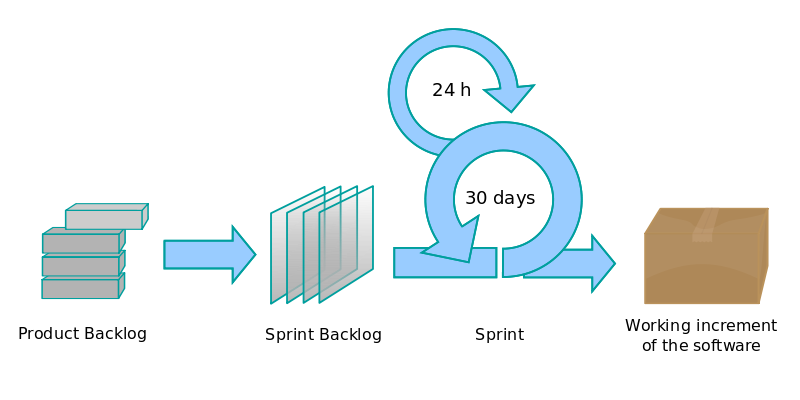
\includegraphics[scale=0.4]{pictures/Scrumprocess.png}
    \caption{Scrum process}
\end{figure}

\subsubsection{Scrum in the project}

This project will not follow the methodology to the letter. The reason for this is that the team do 
not have the opportunity to work together as much as would be preferred, with all members present. This affects
for example the Standup routine. Standups will not be held every day, the way one would do in the scrum,
but when the team sit together every member gives a status report of what they are working on. Even though standups are not held, it is still important to give the other team members a status update.

Allocation of roles has been limited to the Scrum master and the Scrum team where each person in the scrum team has an area of responsability. Sprint planning is run in advance of each sprint and a sprint delivery for the customer 
is held after each sprint. The objective of the sprint delivery is that the customer is able to see the results and progress of the project. During these deliveries the customer has the opportunity to present feedback and changes 
if they want to.

After each sprint a "sprint retrospective" is held to always strive for better working 
process. This allows the group members to give feedback to each other.


\clearpage
\subsection{Group Organization}

In this project we are only 4 people and that will affect how we organize 
the group. We will try to assign roles and responsabilities, but it will
require that each group member has more than 1 role.
In scrum there are mainly 3 roles: product owner, scrum master and the
scrum team. Since we are a small group we will have a overall flat structure. That means that
there will be traditionally project roles that will not be assigned to a specific person, 
but to the group as a whole. It will be the project managers responsability to ensure 
that activities within a unassiged role are covered during the project.

\subsubsection{Roles}

{\bf The Scrum Master (Project manager)} is the responsible person for the progress of the project 
as well as having control on the organizational tasks like planning and workload.
To keep the righ direction of the project, the project manager has to make plans for 
activities like sprints, meetings and deliveries. This include contact with customer and the supervisor.
Before every sprint, meeting and delivery, the project manager has the responsability to book a room, contact all
participants as well as creating the agenda for the meeting. \\

\noindent
{\bf The Scrum Team}
\begin{itemize}

  \item {\bf Test manager:} has the role to ensure the quality of the product. To keep the quality 
  of the product, the test manager has to ensure that each developer create unittests for the 
  produced code, ensure that all the planned test activities is performed and that the results 
  from all test activities is reported.

  \item {\bf Document owner:} has the responsability to allocate task to all the group members so we can meet the deadlines. The document owner does also have the responsability the keep track of what setions in the report to deliver in each sprint and the quality of what we deliver.

  \item {\bf Technical leader:} has the role to ensure that the right technology is
  chosen, have the overview og the version control sytstem and training the group members.

  \item {\bf Development leader:} has the responsability to ensure that we will meet our goals
  for each sprint and that each developer are doing their tasks. The goals are described in each sprint as "features to implement".

  \item {\bf Developer:} each developer has the responsability to produce quality code
  and write unittest for what he/she produce. Every developer do also have the responsability
  to make sure that the produced code that is pushed to the repository is running and working
  according to the requirement specification.
  \end{itemize} 

\subsubsection{Allocation of roles}

\clearpage
\clearpage
\subsection{Project Phases}

The team mainly worked in phases called sprints. In the beginning of the project there were a 2 week period spent on preliminary studies and on planning. The next phases was the sprints (1-4). The sprints were scheduled to last for 2 weeks each with focus on the implementation of the game. The last phase was the delivery and documentation phase, where no new features were to be implemented. The phase will, however, be spent ensuring that all code produced is ready for delivery and finishing the report.

\subsubsection{Planning and research}
In this phase the focus was on getting startet. Every project need roles, a plan and a description of what to deliver. Fitst roles were delegated. After delegating roles the game concept was developed, and the a requirement specification was made. Subsequently it had to be decided what technology to use, which methodology to follow as well as making an overall project plan. 

\subsubsection{Sprints}
This phase of the project is divided into 4 phases that are called sprints and which lasts for 2 weeks. In the sprints the focus is on what features to deliver in the end of the sprint as well as making progress with the report. The sprints and their activities and results are described as own chapters in the report.

\subsubsection{Documentation and delivery}
This phase is the last week of the project. This is the time where no new features will be implemented, but in which it will be made sure that the game is stable and playable. It is also important to finish the final documentation in this phase.

\clearpage
%TODO: add a description of M, H and L in the risk analysis

\pagestyle{fancy}
\clearpage
\section{Risk Management}

This section will focus on the risks that have an attached probability and consequence to the project. If a risk occurs, it is important to have a plan for how to manage the risk and a description of how to act in a proactive and preventive way. Table \ref{table:riskmanagement} shows the risk table that was developed in the start of the project.

Table \ref{table:consequencelevels} and \ref{table:possibilitylevels} describes the attributes 'consequence' 
and 'probability' that are attached to a risk:

\definecolor{gray}{gray}{0.6}

%Consequnce
\begin{table}[H]
\begin{tabular}{| p{3cm} | p{8cm} |}
  \hline
  \rowcolor{gray}
  {\bf Title} & {\bf Description} \\ \hline
    High (H) & A major problem, significant revision in plan or product. 
    A serious delay in deliverables.\\ \hline
    Medium (M) & Project could be delayed, a lot of work to meet deadlines but
    manageable.\\ \hline
    Low (L) & Minor impact on the project, less significant milestones not met.\\ \hline
\end{tabular}
\caption{Description of consequence levels}
\label{table:consequencelevels}
\end{table}

%Probability
\begin{table}[H]
\begin{tabular}{| p{3cm} | p{8cm} |}
  \hline
  \rowcolor{gray}
    {\bf Title} & {\bf Description} \\ \hline
    High (H) & Current circumstances show that the the risk is very 
    likely to occur.\\ \hline
    Medium (M) & Likely to occur.\\ \hline
    Low (L) & Unlikely to occur, and the circumstances likely to trigger 
    the risk are also unlikely to occur.\\ \hline
\end{tabular}
\caption{Description of possibility levels}
\label{table:possibilitylevels}
\end{table}

\pagestyle{empty}
\begin{landscape}
	\addtolength{\oddsidemargin}{-1.1in}
	\addtolength{\topmargin}{0.5in}
  \begin{table}
	\begin{tabular}{| c | p{1.5cm} | p{4cm} | p{4cm} | c | p{4cm} | p{4cm} | c |}
    \hline
    \rowcolor{gray}
   	{\bf Nr} & {\bf Activity} & {\bf Risk factor} & {\bf Consequences} & {\bf Prob.} & {\bf Proactive strategy} & {\bf Reactive actions} & {\bf Responsible} \\ \hline

   	1 & All & Incomplete requirement specification from customer & H: Will result in a late start-up and more work later & M & REDUCE: Contact the customer early in the process. & Complete it ourselves and get approval from customer & Marte \\ \hline

   	2 & All & Samfundet and other voluntary work & M: Decrease in quality of project & H & REDUCE:Make sure we have clearly defined responsibilities & Clarify responsibilities and expectations through conversation & Marte \\ \hline

   	3 & Project delivery & Not reaching the expected quality of the customers expectations & H: Unhappy customer & M & Maintain contact with the customer throughout the project & Try to modify the customer’s expectations, or alter our end product if time allows it & Martin \\ \hline

   	4 & All & Illness & M: More work on others & H & ACCEPT & Postpone or distribute tasks to remaining group members dependent on importance of tasks & Anders \\ \hline

   	5 & Develop- ment and project delivery & Customer is not reachable. & M: May slow down or even halt the work process & L &
   	AVOID: Make clear appointments and keep the customer well informed & Keep trying to reach the customer & Solveig \\ \hline

   	6 & Develop- ment and testing & Other school work & M: Similar to point 2, a decrease in quality due to lowered effort& H & REDUCE: Again, similar to point 2: Make sure we have clear expectations. & 
	Clarify expectations through conversation. & Solveig \\ \hline

   	7 & Develop- ment & Continuous change to requirementsby customer & M: A slower and more stressful work process & M & AVOID: Sign a specification before work begins & Adapt if possible, otherwise refer to the signed specification & Martin \\ \hline

   	8 & Develop- ment and testing & Unforeseen problems with the development platform & 
	M: Slower work process and decreased quality of the end product & M & REDUCE: Do proper research and frequent testing (manual or automated) & Start again from a point where the work looked promising &Anders \\ \hline

   	9 & Develop- ment and project delivery & Unrealistic expectations & H: A difficult development process and an unhappy customer & L & AVOID: Create a clear specification which is approved and signed by both parties & Attempt to adjust the customer’s expectations through conversation & Marte \\
   	\hline
    \end{tabular}
    \caption{Risk Management}
    \label{table:riskmanagement}
    \end{table}
\end{landscape}

\pagestyle{fancy}

\clearpage
\subsection{Quality Assurance}

\subsubsection{Internal reporting/routines}

\subsubsection{Meetings (and interaction?)}

\subsubsection{Templates}

Meeting minutes

Hour list


\subsubsection{Phase Result Approval}

\subsubsection{Response Time Lines}

\subsubsection{Documentation and Code}

\subsubsection{Testing}

Releases And Builds.

Unit Testing.

Functional Testing.

\subsubsection{Task Reviewing and Inspection??}






\clearpage
\section{Preliminary Studies}
This chapter presents the research and studies the group performed during the first phase of the project. The objective was to obtain a good understanding of the problem and which possibilities existed. The first sections looks into possible development methodologies to adapt, and what the best option is for this project. A great part of the planning was to come up with a concept for the game, and process is described in chapter 3.2. The two following sections take a look at Mobile Technology and Mobile Development, respectively, were different options are explored. Finally, in chapter 3.5, different tools that will be of help during the project are presented.
\section{Methodology}

This section describes the study on different methodologies that took place before choosing a methodology
for this project. At the end of this section, there will be a conclusion of what was chosen and why.

\subsection{Waterfall}

{\bf The waterfall process } is a sequential design process that 'flows' through the phases like a waterfall.
The waterfall process is also known as the 'standard' process because it was the most popular process before
agile processes became popular. 

With the waterfall process there is only one distinct goal for each phase. One can imagine a waterfall on the cliff of a steep mountain. Once the water is flowing over the edge of the cliff, it cannot turn back. The same applies to waterfall development. \cite{wikiWaterfall, techtargetWaterfall}

{\bf The phases of the waterfall model:} There are five main phases in a normal waterfall process. 
Here is a brief description:
\begin{itemize}
	\item {\bf Requirement specification:} Is the phase where the requirements are collected, functional and non-functional, to make a complete description of the behaviour of the system to be developed.
	\item {\bf Design: } Is the phase where the requirements are used to make the overall design of the system such as the
	architecture.
	\item {\bf Implementation:} Is where the development of the designed system is done. In the implementation phase, 
	it is also common that some kind of testing takes place during implementation.
	\item {\bf Verification (testing and installation): } When the implementation is done, the solution needs to be tested and installed.
	\item {\bf Maintainance:} Is the modification of a software product after delivery to correct errors, to improve performance or other attributes.
\end{itemize}

{\bf Pros: }
\begin{itemize}
	\item Simple and easy to understand and use
	\item Phases are processed and completed one at a time.
	\item Works in projects where the requirements are well understood (low risk of the requirements being changed)
\end{itemize}

{\bf Cons: }
\begin{itemize}
	\item It is very difficult to change the requirement specification, so it is not suitable for the projects where requirements are at a moderate to high risk of changing.
	\item No delivery of working software until the end of the project. This can be critical because the customer may not
	be able to be a part of the process and this may result in an unhappy customer.
\end{itemize}

\begin{figure}[!ht]
\centering
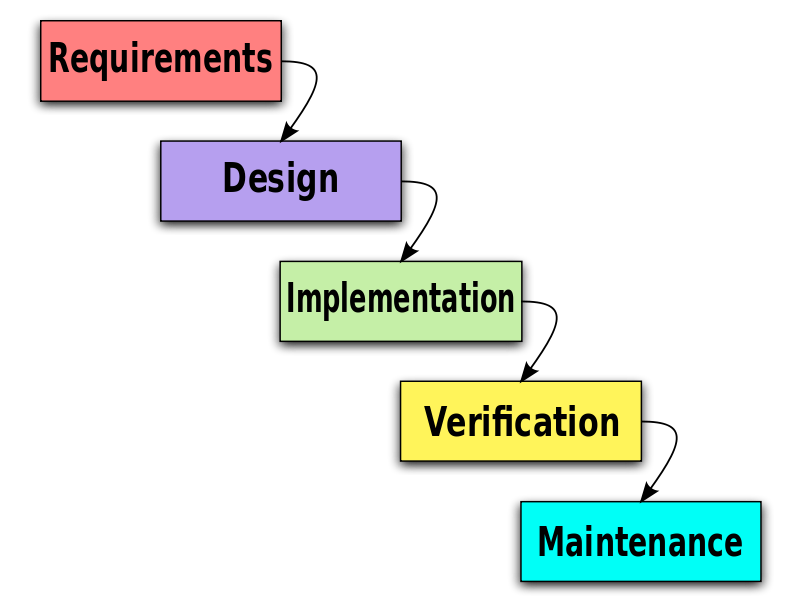
\includegraphics[scale=0.3]{pictures/Waterfall_model.png}
\caption{The waterfall process}
\label{overflow}
\end{figure}


\subsection{Scrum}
{\bf The scrum process: } Scrum is an agile iterative process with focus on small deliveries. The process
defines a self-sustaining team ("The Scrum Team") that defines the goal for each phase. The goal 
is achived through small product increments in iteration that normally last for 1-4 weeks. 
All the functions to implement is planned and is added to a list called a "Product Backlog". The
functions is normally defined as user stories and is added in a prioritized order. In each increment, 
in scrum called a "Sprint", there is a sprint meeting where the scrum team pick userstories from the 
product backlog and add them to the "Sprint Backlog". The sprint backlog is the description of what 
to deliver in the end of the sprint.

Because it is a flat structure there is a concept in scrum called "daily standup". This will keep the team together and everyone will be able to get a quick status update. It usually lasts only 5-15 minutes. 

In a scrum process the stakeholders are a part of the team. The stakeholders will be able to give
feedback in every sprint in terms of changes or approval of a delivery in what is called a "sprint review".
In other methodologies, the stakeholders are only a part of a big delivery in the end, and will 
make it difficult to make changes to what is developed. In scrum, each sprint is a small delivery.

{\bf Pros: }
\begin{itemize}
	\item Small deliveries with feedback from stakeholders
	\item Opportunity to make changes to the requirements during the process
	\item Flat structure (this will adapt to small and bigger teams)
	\item Daily status update from daily standup meetings
	\item Fits for small teams
\end{itemize}

{\bf Cons: }
\begin{itemize}
	\item Require the stakeholders (the customer) to be a part of the team and participate during the process.
\end{itemize}

\subsection{Conclusions}
This section described two different methodologies that were considered as possible methodologies for this project. Because the project is to develop a game with few requirements from the customer, there is a need for a process that will adapt to constant changes in the requirement specification. The waterfall process will not support this and it will be hard to use such a process. The scrum process is more likely to fit this project in terms of the amount of planning, 
number of team members and also the high possibility of changes to the requirements.




\clearpage
\section{Game Concept Development}

This section describes the process of coming up with a concept for the game, as well as where inspiration came from. Initially the group considered the power industry in Norway. Thereafter two quite different game concepts were developed and presented to the customer.

\subsection{The Power Industry}

\begin{wrapfigure}{r}{40mm}
  \begin{center}
  
\includegraphics[scale=0.5]{pictures/water_generator.png}
  \end{center}
\end{wrapfigure}

In Norway 99\% of all power production is generated through hydropower. Hydropower is generated when pressurized water is used to drive a turbine which turns the energy of the water into electricity. When electricity has been produced, it passes through the transformer where it is stepped up to high voltage. Then it is sent onto the power grid. Hydropower is pollution-free and renewable. Because water is often stored in reservoirs, it is also very flexible; electricity can be produced when demand is high. \cite{statkraftVannkraft}

\subsection{The First Game Concept}

During the first meeting with the customer, it was clear that they did not have a very specific idea of what the game should contain beyond what the project description said. The product description says that the game should be focused around controlling power production from hydro plants trough a power grid to the customers, but it could also be centered around something else as long as the theme of hydro power was kept. The conclusion in the first customer meeting, concerning the concept, was that most importantly the game should be fun and something users would want to play. This
lead the group to a phase in which different options for a game concept were considered.

The group's first idea was inspired by games that have a simple concept interface, but that are still fun and addictive, as those games often turns out to be the most popular, e.g. Tetris. In brief the first concept the group came up with was a simple, level based 2d game, where the goal is to serve all customers (nodes) with power produced from the power station
(Helgelandskraft). The nodes are scattered around the screen, and the player draws a line from node to node without lifting his or her finger. There is not unlimited power, so the player needs to find the shortest path to deliver
power to all nodes. If the power station runs out of power before every node is served, the player loose and needs to start the level from scratch.

This idea was presented in the second customer meeting. The customer liked it, but was also unsure whether it was too abstract from what a power plant company actually do. 

\subsection{The Final Game Concept}

Following this meeting the customer was asked to come up with a more specific concept of their own, and the group would also look at other options for a game concept. The second game concept had more base in reality. Briefly explained, the player is in charge of the electric utility in town and has the responsibility of supplying the inhabitants and local industry with electricity by building power plants and power lines. When brainstorming for this concept the group began to look to construction and management simulation games, as this could be a good way to present an industry and how it works as well as create a fun and challenging game. At the following customer meeting both the groups and the customers ideas were presented. The final game concept was decided during this meeting. A more detailed description of the final game concept can be found in Chapter \ref{chap:gameconsept} Game Concept. The customer was happy with this concept as it was closer to what the product description explained and more realistic.

\subsection{Similar game concepts}

{\bf Construction and management simulation games}

Construction and management simulation games, hereafter called CMS games, are based on building, managing and expanding virtual communities or projects with limited resources. CMS games have been developed since the 1980s and continue to be popular to this day. SimCity, which was released in 1989 and is considered to be the first CMS game to be highly successful, has spawned numerous successors, the last one released this year. \cite{wikiCMS}

{\bf Megapolis}

One specific game that the group took a closer look at was the Megapolis game developed by Social Quantum for the iPhone and iPad. This is a construction and management simulation game in which the player builds his own virtual city. As the person in charge of the city the player needs to manage the finances of the city, provide it with water and electricity, and develop infrastructure such as airports and power plants. The goal is to keep expanding the city, unlock new tasks and rewards and build the most impressive city. \cite{megapolis}

\begin{figure}[H]
	\centering
	
\includegraphics[width=\textwidth]{pictures/megapolis.jpg}
	\caption{Game: Megapolis}
\end{figure}

The group found a number of other CMS games when searching through AppStore and GooglePlay, but none in which power production and power supply were a major part of the game. This does however prove that there is an interest for games
with elements of CMS.

Finding games with elements of power supply and production proved to be more difficult.

\subsection{Conclusions}

The group decided to develop a construction and management game, dubbed Power Supply. CMS games are very popular, both as more dedicated games like SimCity and casual games like Megapolis, and a point the customer was very clear about was that they primarily wanted people to play the game. Developing a game in a genre that is widely popular made sense. It is also a genre that the group members are familiar with playing. The final game concept is described in Chapter \ref{chap:gameconsept} Game Concept.

\clearpage
%TODO: add intro to the sections
\subsection{Mobile technology}

After the introduction of smartphones, there has been an explosive surge in the
popularity of using mobile technologies as computers.
\begin{figure}[!ht]
\centering
\subfigure{
  
\includegraphics[scale=0.06]{pictures/android}
}
\subfigure{
  
\includegraphics[scale=0.2]{pictures/apple-logo}
}
\subfigure{
  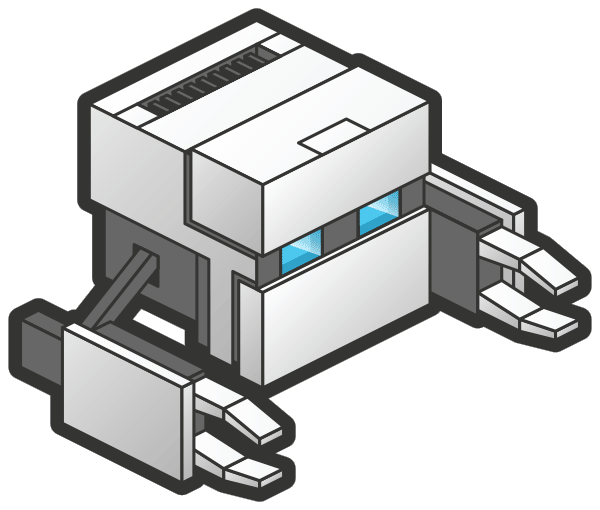
\includegraphics[scale=0.1]{pictures/phonegap}
}
\subfigure{
  
\includegraphics[scale=0.13]{pictures/css3}
}
\linebreak
\subfigure{
  
\includegraphics[scale=0.245]{pictures/html5}
}
\subfigure{
  
\includegraphics[scale=0.12]{pictures/corona}
}
\subfigure{
  
\includegraphics[scale=0.25]{pictures/js}
}
\caption{Android, IOS, Phonegap, CSS3, HTML5, Corona and Javasript}
\end{figure}

\subsubsection{Mobile platforms}
{\bf Android} is a Linux-based operating system, designed primarily for mobile
devices with touch screen support. Android is currently being developed by
Google and is deployed on various mobile devices developed by third parties.
[http://en.wikipedia.org/wiki/Android_(operating_system)]
\linebreak

\indent
  {\bf Pros:}
  \begin{itemize}
    \item Developing for Android is free.
    \item Native support for Java, a well known programming language.
    \item Android apps can be developed on any of the major desktop operating
          systems.
    \item Android can be emulated using an AVD (Android Virtual Device),
          allowing for easy testing.
  \end{itemize}

\indent
  {\bf Cons:}
  \begin{itemize}
    \item There are many different Android devices, making testing more
          demanding.
    \item Apps developed for Android will only run on Android.
  \end{itemize}

\noindent
{\bf iOS} is an operating system developed by Apple primarily for the iPhone,
which has been extended to run on other Apple devices such as the iPad. Apple
does not allow iOS to be deployed on non-Apple hardware.
[http://en.wikipedia.org/wiki/IOS]

\indent
  {\bf Pros:}
  \begin{itemize}
    \item There are fewer devices running iOS, and things like screen
          resolution is typically standardized, making development and testing
          easier.
  \end{itemize}

\indent
  {\bf Cons:}
  \begin{itemize}
    \item Apple hardware and software required to develop for iOS.
    \item Distribution of applications for iOS requires a yearly subscription.
    \item Apple's App Store enforces strict terms of distribution which may not
          be compatible with other software licences.
    \item Apps developed for iOS will only run on iOS.
  \end{itemize}


\subsubsection{Cross-platform}
{\bf PhoneGap} is a free and open source framework that makes it possible
to create mobile applications using web technologies like HTML, CSS and
JavaScript. PhoneGap allows developers to create an application which is a
hybrid between a web app and a native application. PhoneGap packages the
program as an application and gives the developer access to native device APIs.
[http://phonegap.com/about/]

\indent
  {\bf Pros:}
  \begin{itemize}
    \item Applications can be developed for Android, BlackBerry, iOS,
          Windows Phone, Windows 8 and Tizen operating systems.
    \item PhoneGap apps are developed using well known technologies such as
          JavaScript, HTML and CSS.
    \item Access to native APIs like camera, storage, networking,
          touch screen etc.
    \item Existing CSS and JavaScript libraries can be leveraged.
    \item Looks like a native application.
    \item Makes it easy to build applications for all supported platforms.
    \item PhoneGap is open source.
  \end{itemize}

\indent
{\bf Cons:}
  \begin{itemize}
    \item PhoneGap runs as an offline webpage, which is likely to impact
          performance.
  \end{itemize}

\noindent
{\bf Corona} is a software development kit (SDK) which allows developers to
build applications for iPhone, iPad and Android devices. Corona is not open
source, and enforces a revenue limit for developers unless the developers pay a
monthly fee. Corona lets programmers develop using Lua.
[http://www.coronalabs.com/products/corona-sdk/]

\indent
  {\bf Pros:}
  \begin{itemize}
    \item Comes with a physics engine and other features useful for game
          development.
  \end{itemize}

\indent
  {\bf Cons:}
  \begin{itemize}
    \item Not open source
    \item Costs money to unlock full feature set.
  \end{itemize}

\subsubsection{Native}
For focus on single platforms, developing native applications would probably be
the best choice. Native applications for Android are developed using the Java
programming language whereas iOS apps are developed in Objective-C.

\indent
  {\bf Pros:}
  \begin{itemize}
    \item Easier to ensure that the application will run on all versions of
          the platforms.
    \item Best performance.
  \end{itemize}

\indent
  {\bf Cons:}
  \begin{itemize}
    \item We have to develop for both iOS and Android in different languages.
          Both of these apps would have to be maintained in parallel.
    \item We will have to learn Objective-C.
    \item Can only build applications for iOS on Mac.
  \end{itemize}

\noindent
\subsubsection{Conclusions}
After having discussed it in the group and with the customer we have agreed
on using PhoneGap to develop the game. The customer wanted the game to
be developed with known technology that they can easily find people with
experience with. HTML, CSS and JavaScript constitute a very popular development
platform.

\clearpage
\subsection{Mobile development}

\subsubsection{Native languages}
\subsubsection{JavaScript, HTML5, and CSS3}
\subsubsection{Frameworks}
\subsubsection{Conclusions}
This is a very important conclusion!

\clearpage
\subsection{Tools}

\clearpage
\section{Game Concept}
\subsection{Introduction}
\subsection{About}
Game concept is a detailed description of the game, including information such as high concept, genre,
gameplay description, features, setting, story, target audience, hardware platforms, estimated schedule,
marketing analysis, team requirements and risk analysis. Source: 
\url{en.wikipedia.org/wiki/Game_development#Development_process}
Several of these points like the risk analysis and hardware platforms have been brought up in other 
sections of the report and will not be discussed here. This section will mainly be about the gameplay. 
The game concept is the basis for the game's functional requirement. It is easier to explain the game 
as well as decide on the functional equirements for the game on the basis of the game concept. 

\subsection{High Concept}
The name for the game we settled on is Power Supply. It is in the construction and management 
simulation genre and is inspired by games like SimCity, only in a more limited scope. You are 
tasked with managing the delivery of electricity to cities and factories in an area, while the 
ultimate goal of the game is making money as the tycoon of the local power company, without going 
bankrupt.

\subsection{Gameplay Description}

\subsubsection{Player}
The role of the player is to build powerplants to supply the buildings on the game map with power. 
To do this the player has to connect the powerplants to the buildings with powerlines. Either directly
or indirectly. Building powerplants and powerlines costs money. To earn money the player has to supply
power to the buildings on the map. If the inhabitants of a building does not get power then they will
move out and abandon the building. If too many buildings become abandoned then the game is over.
Abandoned buildings disappear from the game.

\subsubsection{Powerplants}
Powerplants can only supply a fixed amount of power to the connected buildings. If a powerplant is 
unable to supply power to all the buildings on the map, the player has three options. The first option 
is to build more powerplants. The second powerplant can then be connected to the buildings that the
player wasn't previously able to supply with power. The second option is to upgrade the powerplant,
so that it can deliver more power. This is supposed to be more cost effective in the short term, however
it can become more expensive in the long run because of other important factors which will be brought
up later. The final option is to demolish an already existing powerline and allow the powerplant to
supply another building with power. This could be risky, as buildings that are not supplied with power
will eventually become abandoned.

\subsubsection{Powerlines}
Powerlines is the way the player connects their powerplants to the buildings in need of power. This 
can be done directly or indirectly. A direct connection is a connection between a powerplant and a 
building in need of power. While an indirect connection is to connect a building with another building.
Power from the powerplant then travels through the directly connected powerlines and continues down 
the indirectly connected powerlines, supplying as many buildings as possible with power. Direct 
connections are important, since buildings that are directly connected will receive power first.
However you also have to consider the length of the powerline, as longer powerlines are more expensive
to build than short powerlines. You can also tear down powerlines in order to supply other buildings
with power.

\subsubsection{Buildings}

\subsubsection{Goal}


%ohmville, spillrolle, elementer, mål, oppgaver, hindringer, levler, etc.

\clearpage
\section{Requirement specification}
\section{Requirements}

This section presents all the functional requirements, as well as the quality requirements.

{\bf Functional requirements:} State what the system must do, how it must behave or react 
to run-time stimuli. \cite{functionalRequirement} \\
{\bf Quality attribute requirements:} Annotate (quantify) functional requirement, e.g. how fast 
the function must be performed, how resilient it must be to erroneous input, how easy the 
function is to learn, etc. \cite{nonFunctionalRequirement}

{\bf The priority scale}:
\begin{itemize}
	\item {\bf Critical:} When a requirement is critical, it means that if the requirement is
	not fullfilled, the game will not be able to work properly. These requirements are of the
	type "need to have".
	\item {\bf High:} When a requirement is highly prioritized, it is important that it will
	be fullfilled in order to make the game work properly, but it will still work without it.
	These requirements are of the type "need to have".
	\item {\bf Medium: } In order to make the game fun and playable it is important that these are 
	fullfilled. This is more like a "nice to have" than "need to have".
	\item {\bf Low:} All the requirements that have a low priority are requirements that are "nice to have",
	but the game will work fine without them. If the project don't have time to implement all
	requirements, the requirements with low priority are the first to go.
\end{itemize}

{\bf The complexity scale:}
\begin{itemize}
	\item {\bf High:} A requirement are set with high complexity if the requirement takes a long 
	time to implement, are dependent on other requirements and/or if the developers do not know
	how to solve the implementation of the requirement.
	\item {\bf Medium:} A requirement are set with medium complexity if the requirement takes 
	some effort to implement, and is dependent on other requirements.
	\item {\bf Low:} A requirement are set with low complexity if the requirement do not take
	a long time to implement, the solution of the implementation is known and/or the requirement
	is not dependent on many other requirements.
\end{itemize}
\section{Functional requirements}

\begin{longtable}{| p{1.5cm} | p{8cm} | p{1.5cm} | p{2cm} |}
\hline
\rowcolor{gray} 
\bf{ID} & \bf{Requirement} & \bf{Priority} & \bf{Complexity} \\ \hline
\multicolumn{4}{|>{\columncolor[gray]{.8}}l|}{1) Basic functionality} \\ \hline
   FR1.1 & The user should be able to read game instructions from the main menu & H & L \\ \hline

   FR1.2 & The user should be able to exit the game at any time, and the game state should 
   be saved and loaded when the user returns to the game & H & M \\ \hline

   FR1.3 & The user should be able to restart any level at any given point of time after start 
   playing & M & L \\ \hline

   FR1.4 & The user should get a highscore based on the time spent finishing the level & M & M \\ \hline

   FR1.5 & The user should be able to improve the highscore on any level by beating previous 
   highscores & M & L \\ \hline

   FR1.6 & The user should be able to pause the game at any time & M & L \\ \hline

   FR1.7 & The game should play background music & L & H \\ \hline

   FR1.8 & The user should be able to turn on/off the background music & L & L \\ \hline

\multicolumn{4}{|>{\columncolor[gray]{.8}}l|}{2) Building and Upgrade} \\ \hline

   FR2.1 & Buildings should appear around the map at arbitrary intervals and locations & C & H \\ \hline

   FR2.2 & The user should be able to buy and place several power stations on the game map & C & H \\ \hline

   FR2.3 & The user should be able to buy and place power cables on the map & C & H \\ \hline

   FR2.4 & The user should be able to connect the buildings to the powerplants by building a power 
   cable & C & H \\ \hline

   FR2.5 & The user should be able to upgrade the power plant & H & M \\ \hline

   FR2.6 & The amount of power available to the user should be limited; the power supply of a 
   power plant should be upgradeable. & H & L \\ \hline

   FR2.7 & The user should be able to remove power lines from the map & M & M \\ \hline

   FR2.8 & The player should only be allowed to build a level-specific number of power plants. & M & L \\ \hline

   FR2.9 & The user should be able to see information about buildings when tapping on them. & M & M \\ \hline
\pagebreak
\hline
\multicolumn{4}{|>{\columncolor[gray]{.8}}l|}{3) Obstacles} \\ \hline

   FR3.1 & Arbitrary power lines may be damaged throughout the game & M & M \\ \hline

   FR3.2 & The user should be able to fix unstable power lines before it is broken; 
   this should cost some amount of money. & M & L \\ \hline

   FR3.3 & FR3.3 There should be several types of buildings on the map, with different power 
   requirements & M & H \\ \hline

   FR3.4 & Different types of building should reward different amounts of money & 
   M & H \\ \hline

   FR3.5 & The user should be informed about new obstacles & M & M \\ \hline

   FR3.6 & The user should be able to see that a building has gone without power 
   for some time, and is affecting the player's health score & C & M \\ \hline

\multicolumn{4}{|>{\columncolor[gray]{.8}}l|}{4) Level specific} \\ \hline

   FR4.1 & The user should be able to continue to the next level when the goal is reached & H & L \\ \hline

   FR4.2 & The user should be able to continue a level while the health score is greater than zero. 
   When the health score reaches zero, the game is over. & H & L \\ \hline

   FR4.3 & When an existing building is not supplied with power, the player's health 
   score should decrease & H & M \\ \hline

   FR4.4 & As the user reaches higher levels new buildings appear more rapidly & M & H \\ \hline

   FR4.5 & As the user reaches higher levels unstable power lines will appear more rapidly & M & H \\ \hline

   FR4.6 & As the user reaches higher levels the map size may increase & L & H \\ \hline

\multicolumn{4}{|>{\columncolor[gray]{.8}}l|}{5) Incoming/outgoing money:} \\ \hline

   FR5.1 & The user should be able to collect money from the buildings connected to the power plant & H & L \\ \hline

   FR5.2 & When connecting buildings through power cables, there should be a cost which is proportional 
   to the length of the cable. & H & L \\ \hline
\pagebreak
\hline
\multicolumn{4}{|>{\columncolor[gray]{.8}}l|}{6) GUI} \\ \hline

   FR6.1 & The user should be able to see a small part of the game map. & C & L \\ \hline

   FR6.2 & The user should be able to navigate around the map using the touch function on the phone & C & M \\ \hline

   FR6.3 & The user should be able to click on a power plant to receive information about the cost 
   of upgrading it and what the upgrade does & M & M \\ \hline

   FR6.4 & The user should be able to view all of the map by double tapping the screen; double tapping a 
   point on the complete map should zoom in on that area. & M & H \\ \hline

   FR6.5 & The user shoud get a notification of new events outside the screen & L & M \\ \hline

   FR6.6 & A power preservation tip should appear when the user reaches a new level. & L & L \\ \hline

\hline
\caption{Functional Requirements}
\end{longtable}

\clearpage
\definecolor{gray}{gray}{0.6}
\section{Quality Requirements}

This section describes the quality requirements for the game and will briefly describe all requirements under each quality requirement. Each requirement will be described with a quality attribute scenario that looks like this:

\begin{itemize}
	\item {\bf Source of stimulus:} Human, computer, or other actor that generates the stimulus
	\item {\bf Stimulus:} Condition that needs to be considered when it arrives at a system
	\item {\bf Environment:} The stimulus occurs within certain conditions
	\item {\bf Artifact:} Some artifact is stimulated 
	\item {\bf Response:} The activity undertaken after the arrival of the stimulus
	\item {\bf Response measure:} When the response occur, it should be measured in some fashion so that the requirement can be tested.
\end{itemize}

\begin{figure}[!hr]
	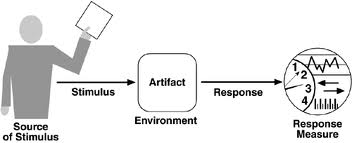
\includegraphics{pictures/qualityAttribute.jpg}
	\caption{Quality attribute scenario}
\end{figure}

{\bf What is a quality attribute?:}

{\bf Priority of quality attributes:} It is not possible to meet all quality requirements because some decisions will affect others. This will result in a priority of the quality attributes that we need to meet and some that are less important. We have picked two main quality attributes: Modifiability and performance.

\begin{itemize}
	\item {\bf Primary quality attribute: } Modifiability
	\item {\bf Secondary quality attributes: } Performance
\end{itemize}


\subsection{Modifiability}

Modifiability is about the cost of change. It brings up two concerns: What can change (the artifact)? 
When is the change made and who makes it (the environment)? 
Once a change has been specified, the new implementation must be designed, 
implemented, tested, and deployed. All of these actions take time and money, both of which can be measured.
Helgelandskraft (the customer) wanted the possibility for further development on the game. The developers
have to keep in mind that the game is developed in a such way that the customer can continue
the development after the delivery. If the game is made in a way that changes are hard to implement, 
the customer would need to use a lot of resources in sense of time and money, and that is the main 
reason for this to be the primary quality attribute.

Changes the customer might want to add to the game is more buildings and more obstacles to take
the game to a more complex state. Good models have therefore been added so that it will be easy for 
the customer to make further development on this part.

\subsection*{M1: Add new elements}
In the game a small set of elements like powerplants, houses, powerlines, etc. has been specified.
In order to have the oppertunity to add new buildings a model for each element with specific attributes has been made. When a developer wants to add more elements, he or she can use these models and easily add the wanted parameters. 

\begin{table}[H]
\begin{tabular}{| l | l |}
	\hline
	\rowcolor{gray}
	{\bf Portion of scenario} & {\bf Values} \\ \hline
	Source of stimulus & Developer\\ \hline
	Stimulus & Add new elements to the game\\ \hline
	Environment & Design time \\ \hline
	Artifact & Code \\ \hline
	Response & Modification is made with no side effects\\ \hline
	Response Measure & 1 hour\\ \hline
\end{tabular}
\caption{Modifiability scenario}
\end{table}

\subsection* {M2: Increase game difficulty}
If the game is made to easy for the user it is possible for the developer to adjust the
parameters in the models. The difficulty of the game is based on these parameters.

\begin{table}[H]
\begin{tabular}{| l | l |}
	\hline
	\rowcolor{gray}
	{\bf Portion of scenario} & {\bf Values} \\ \hline
	Source of stimulus & Developer\\ \hline
	Stimulus & Modify the difficulty in the game\\ \hline
	Environment & Design time \\ \hline
	Artifact & Code \\ \hline
	Response & Modification is made with no side effects\\ \hline
	Response Measure & 1 hour\\ \hline
\end{tabular}
\caption{Performance scenario}
\end{table}

\subsection{Performance}

\subsection*{P1: Rendering (Repaint)}
When changes occure to the game models, the screen should identify if the change 
is visible on the screen. If the change can be seen, the screen should repaint 
that part of the display at the beginning of the next game update.

\begin{tabular}{| l | l |}
	\hline
	\rowcolor{gray}
	{\bf Portion of scenario} & {\bf Values} \\ \hline
	Source of stimulus & Game models\\ \hline
	Stimulus & Change to the internal state of game model\\ \hline
	Environment & Game run time \\ \hline
	Artifact &  Game \\ \hline
	Response & Identify visibility of state change\\ \hline
	Response Measure & Less than 16 ms\\ \hline
\end{tabular}

\subsection{Other Quality attributes}
\subsection*{Usability: } The group do not have the main focus on this quality attribute, but because this is a game that is supposed to be played by a variety of people, it has to be considered to make the game easy to use. Instructions in the main menu has been added to help the user get started.

\subsection*{Testability: } Since the game is made as a prototype, the focus has been on having
test on the main functionality so the customer can run test under further developing.
In order to have test, testable code needs to be written.

\subsection*{Compitability: } The game has to run on different kinds of platforms. A cross-platform framwork has been chosen for development to make it it easier to adapt to new platforms.

\clearpage
\subsection{Userstories}

This section will focus on the user stories in the game. Each story will be 
desribed as a scenario. All the scenarios have a certain number of attributes:
actors, preconditions, flow of events and exceptions.
Before describing the flow of events, you need to know who is involved in the 
scenario (the actors) and what preconditions that needs to be fullfilled before
the scenario can take place. 
In the flow of events, it will be described step by step the actions that can be
carried out and where in the flow you jump if you perform a action.
If any step in the flow of events can occur, it is described in the buttom of each
table. This is events that can occur, but it is not a consistent part of the flow. \\

\definecolor{lightgray}{gray}{0.9}

\begin{tabular}{| l | p{10cm} |}
	\hline
	\rowcolor{lightgray}
	{\bf Scenario \#1:} & {\bf Build Power Plant.} \\ \hline
	Actors: & Player \\ \hline
	Preconditions: & User has initiated a game. \\ \hline
	Flow of events: &  \\ \hline
	1 & The player drags the build menu into view. \\ \hline
	2 & The player taps the Power Plant button. \\ \hline
	3 & The system checks whether or not the player is able to afford the Power Plant. \\ \hline
	4 & The player chooses where to place the Power Plant by tapping the spot on the map where he or she wants it. \\ \hline
	5 & The player is asked to either buy it or decline. \\ \hline
	5.1 & The player taps 'OK'. Go to 6. \\ \hline
	5.2 & The player taps 'Cancel'. Go to 8. \\ \hline
	6 & The system places a Power Plant at det given spot. \\ \hline
	7 & The system reduces the amount of money the player has by the cost of the Power Plant. \\ \hline
	8 & End scenario. \\ \hline
	Exceptions: & \\ \hline
	3.2 & The player is not able to afford the Power Plant. A message is displayed, to let the player know. \\ \hline
	4.1 & The player taps a spot where a building, a Power Line or another Power Plant is already placed. Sound notification. Go to 4. \\ \hline
\end{tabular}

\begin{tabular}{| l | p{10cm} |}
	\hline
	\rowcolor{lightgray}
	{\bf Scenario \#2:} & {\bf Build Power Line.} \\ \hline
	Actors: & Player \\ \hline
	Preconditions: & User has initiated a game. There exists at least one Power Plant and at least on building on the map. \\ \hline
	Flow of events: & \\ \hline
	1 & The player drags the build menu into view. \\ \hline
	2 & The player taps the Power Line button. \\ \hline
	3 & The system checks whether the maximum number of Power Plants has been met. \\ \hline
	4 & The system checks whether the player is able to afford the Power Line. \\ \hline
	4.1 & The player is asked to either buy it or decline. \\ \hline
	4.1.1 & The player taps 'OK'. Go to 5. \\ \hline
	4.1.2 & The player taps 'Cancel'. Go to 9. \\ \hline
	5 & The player chooses the Power Plant to build from by tapping it. \\ \hline
	6 & The player drags a line from the Power Plant to the building to serve. \\ \hline
	7 & The system places a Power Line where the player dragged the line. \\ \hline
	8 & The system reduces the amount of money the player has by the cost of the Power Line. \\ \hline
	9 & End scenario. \\ \hline
	Exceptions: & \\ \hline
	3.1 & The maximun number of Power Plants has been met. A message will be displayed. \\ \hline
	4.2 & The player is not able to afford the Power Line. A message is displayed. \\ \hline
	5.1 & The player does not tap a Power Plant. Sound notification. Go to 5. \\ \hline
	6.1 & The player does not drag the Power Line to a building. Sound notification. Go to 4. \\ \hline
	6.2 & The Power Plant does not have the power to serve this building. Display message to player. Go to 9. \\ \hline
	6.3 & The building is already served by a Power Plant. Display message to player. Go to 9. \\ \hline
\end{tabular}

\begin{tabular}{| l | p{10cm} |}
	\hline
	\rowcolor{lightgray}
	{\bf Scenario \#3:} & {\bf Repair damaged Power Line.} \\ \hline
	Actors: & Player \\ \hline
	Preconditions: & User has initiated a game. There exists a damaged Power Line on the map. \\ \hline
	Flow of events: & \\ \hline
	1 & The player taps the damaged Power Line. \\ \hline
	2 & The system asks whether the player wants to 'Remove' or 'Repair' the Power Line, or 'Cancel'. \\ \hline
	2.1 & The player taps 'Repair'. Go to 3. \\ \hline
	2.2 & The player taps 'Cancel'. Go to 4. \\ \hline
	3 & The system checks whether the player is able to afford the repair cost. \\ \hline
	3.1 & The player can afford the repair cost and the damaged Power Line is replaced by a new. \\ \hline
	4 & End scenario. \\ \hline
	Exceptions: & \\ \hline
	1.1 & The player does not tap a damaged Power Line. Notification Sound. Go to 1. \\ \hline
	3.2 & The player cannot afford the repair cost. A message is displayed. Go to 4 \\ \hline
\end{tabular}

%Koster penger?
\begin{tabular}{| l | p{10cm} |}
	\hline
	\rowcolor{lightgray}
	{\bf Scenario \#4:} & {\bf Upgrade Power Plant} \\ \hline
	Actors: & Player \\ \hline
	Preconditions: & User has initiated a game. A Power Plant is ready to be upgraded. \\ \hline
	Flow of events: & \\ \hline
	1 & The player taps the Power Plant ready to be updated. \\ \hline
	2 & The system displays an information box belonging to the given Power Plant. \\ \hline
	3 & The player taps 'Upgrade' in the information box. \\ \hline
	4 & The system asks whether the player wants to Upgrade the Power Plant \\ \hline
	4.1 & The player taps 'Upgrade'. Go to 5. \\ \hline
	4.2 & The player taps 'Cancel'. Go to 7. \\ \hline
	5 & The system checks whether the player is able to afford the Upgrade. \\ \hline
	6 & The system incerases the amount of power the Power Plant is able to supply. \\ \hline
	7 & End scenario. \\ \hline
	Exceptions: & \\ \hline
	4.1 & The player is not able to afford the Upgrade. A message is displayed. Go to 7 \\ \hline 
\end{tabular}

\begin{tabular}{| l | p{10cm} |}
	\hline
	\rowcolor{lightgray}
	{\bf Scenario \#5:} & {\bf Navigate around the map.} \\ \hline
	Actors: & Player \\ \hline
	Preconditions: & The user has initiated a game. \\ \hline
	Flow of events: & \\ \hline
	1 & The player drags his finger over the screen to navigate. \\ \hline
	2 & The player double taps the screen to zoom out or zoom in. \\ \hline
	3 & End scenario. \\ \hline
	Exceptions: & \\ \hline
	1.1 & The player tries to navigate outside the map. Nothing happens. \\ \hline
\end{tabular}

\begin{tabular}{| l | p{10cm} |}
	\hline
	\rowcolor{lightgray}
	{\bf Scenario \#6:} & {\bf Pause the game} \\ \hline
	Actors: & Player \\ \hline
	Preconditions: & A game has been initiated. \\ \hline
	Flow of events: & \\ \hline
	1 & The player pauses the game. \\ \hline
	1.1 & The player taps the Pause button. \\ \hline
	1.2 & The player leaves the game. \\ \hline
	2 & The system saves the state of the game, \\ \hline
	3 & The player resumes the game. \\ \hline
	3.1 & The player taps the 'Resume' button \\ \hline
	3.2 & The player taps 'Load Game' from Game Menu \\ \hline
	4 & The system returns to the saved game. \\ \hline
	5 & End scenario. \\ \hline
	Exceptions: & \\ \hline
\end{tabular}

\begin{tabular}{| l | p{10cm} |}
	\hline
	\rowcolor{lightgray}
	{\bf Scenario \#7:} & {\bf Remove Power Line} \\ \hline
	Actors: & Player \\ \hline
	Preconditions: & A game has been initiated. There exists a Power Line on the game map. \\ \hline
	Flow of events: & \\ \hline
	1 & The player taps the Power Line he wants to remove. \\ \hline
	2 & The system asks whether the player wants to 'Remove' or 'Repair' the Power Line, or 'Cancel' \\ \hline
	3.1 & The player taps 'Remove'. Go to 4. \\ \hline
	3.2 & The player taps 'Cancel'. Go to 6. \\ \hline
	4 & The system checks whether the playe is able to afford to remove the Power Line \\ \hline
	5 & The system removes the Power Line. \\ \hline
	6 & End scenario. \\ \hline
	Exceptions: & \\ \hline
	4.1 & The player can not afford to remove the Power Line. Display message. Go to 6. \\ \hline
\end{tabular}

\begin{tabular}{| l | p{10cm} |}
	\hline
	\rowcolor{lightgray}
	{\bf Scenario \#8:} & {\bf Get information about building} \\ \hline
	Actors: & Player \\ \hline
	Preconditions: & A game has been initiated. There exists a building on the map. \\ \hline
	Flow of events: & \\ \hline
	1 & The player taps the building he wants more information about. \\ \hline
	2 & The system displays a box with information. \\ \hline
	3 & The player taps 'OK' when he is done. \\ \hline
	4 & End scenario. \\ \hline
	Exceptions: & \\ \hline
	1.1 & The building is ready to pay for the power. The player must collect money before information is shown. \\ \hline
\end{tabular}

\begin{tabular}{| l | p{10cm} |}
	\hline
	\rowcolor{lightgray}
	{\bf Scenario \#9:} & {\bf Building is not served with power.} \\ \hline
	Actors: & Player \\ \hline
	Preconditions: & A game has been initiated. At least one house is not connected to a Power Plant. \\ \hline
	Flow of events: & \\ \hline
	1 & The house's timer starts going. \\ \hline
	1.2 & The player does not connect the house to a Power Plant. Go to 2. \\ \hline
	1.2 & The player connects the house to a Power Plant. The timer stops and is set to 0. Go to 5 \\ \hline
	2 & The timer reaches a certain point \\ \hline
	3 & The building is removed. \\ \hline
	4 & The player's Healthbar decreases with a certain amount. \\ \hline
	4.1 & The system checks whether the Healthbar is below 0. \\ \hline
	4.1.1 & The Healthbar is not below 0. Go to 5 \\ \hline
	4.1.2 & The Healthbar is below zero. Game Over. \\ \hline
	5 & End scenario. \\ \hline
	Exceptions: & \\ \hline	
\end{tabular}

\begin{tabular}{| l | p{10cm} |}
	\hline
	\rowcolor{lightgray}
	{\bf Scenario \#10:} & {\bf Collect money from building.} \\ \hline
	Actors: & Player \\ \hline
	Preconditions: & The game has been initiated. There exists a building on the map. The building is ready to pay for the power. \\ \hline
	Flow of events: & \\ \hline
	1 & The system shows that the building is ready to pay for the power. \\ \hline
	2 & The player taps the building he wants to collect money from. \\ \hline
	3 & The sytems updates the players money. \\ \hline
	4 & The system checks whether the player has reached the goal. \\ \hline
	4.1 & The player has reached the goal and is sent to the next level. \\ \hline
	4.2 & The player has not reached the goal. \\ \hline
	5 & End scenario. \\ \hline
	Exceptions: & \\ \hline
\end{tabular}
\clearpage
\section{Use Case Diagrams}

This section outlines the use cases for the product. Standard UML notation is used. There are 4 elements, the actor who interacts with the system, the use cases, that are tasks that can be performed by the system, and lines that represent relationships between the actor and the system. The fourth element is the system or application itself, which is not viualized here, but which is made up of all the use cases in the given diagram. The lines that are marked "include" are used to show the relationship between use cases where one can be reached from the other. \cite{usecaseUML}


\begin{figure}[H]
  	\centering
	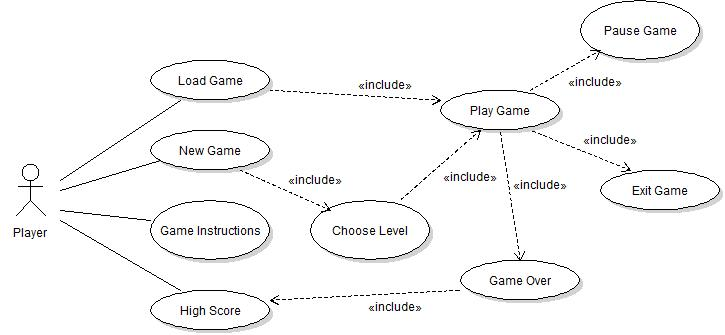
\includegraphics[scale=0.45]{pictures/UCD_Game_Menu_After.jpg}
	\caption{Use Case Diagram of Game Menu}
\end{figure}

\begin{figure}[H]
  	\centering
	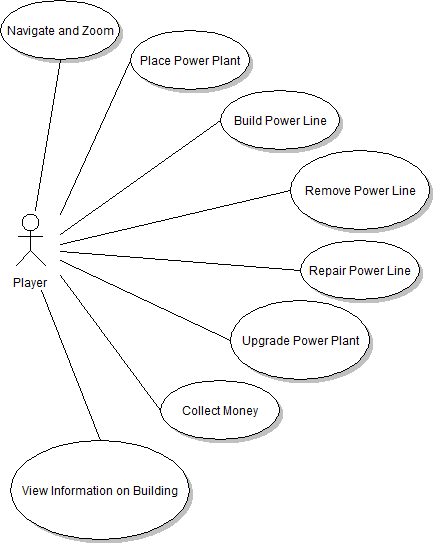
\includegraphics[scale=0.5]{pictures/UCD_PlayGame.png}
	\caption{Use Case Diagram of Gameplay}
\end{figure}


\clearpage
\section{Hour Estimation}

	This section describes what hour estimation is, how to perform it and how we
	included it in our project. The actual estimated hours are not done in this section, 
	but is documented in each sprint section.

	{\bf What is hour estimation?} Hour estimation is performed as a part of a project in order to ensure that 
	one have the resources necessary to complete a project in time. Hour estimation can be done in many different 
	ways, but often depends on the methodology	used in the project. In a waterfall project, it is common to do all 
	the estimation in the start of a project. When a project uses agile methods like scrum, it is common to do 
	the estimation partin each sprint. \cite{estimation}

	{\bf Why perform hour estimation?} In software projects, the projects normally starts with
	a planning phase and an hour estimation. There are several reasons as to why this estimation is done:
		\begin{itemize}
			\item Calculate the cost for delivering a project.
			\item Calculation resources for a project (e.g how many people do the team 
			need for this project?).
			\item How many features can the team implement during a phase/sprint?
			\item Are the project in time (the estimated hours in the backlog)?
			\item How big is this project in terms of hours?
		\end{itemize}
	There are many good reasons for doing an estimation, but the reasons are often dependent
	on the methodology used and the purpose of the project. 

	If no estimation has been performed in a project, there are many risk factors that can appear:
	\begin{itemize}
		\item If a company win a project and promises the customer to deliver at a 
		specified date without estimating hours for the project, there is a big risk 
		that the project will fail.
		\item If a project has not estimated the hours, there is a possibility that 
		there is not allocated enough resources for the project, and the project could 
		be risking not to be delivered at the planned date.  
	\end{itemize}

	{\bf How we performed hour estimation} This project have like many other projects a deadline
	as well as a specified number of resources. In many projects it is normal to set the wanted 
	delivery and then estimate the number of resources needed to deliver the project.
	In this project we started with a number of resources (4 students) and then planned the 
	delivery based on the workload of the course (ca 24 hours/persons/week). The actual 
	hour estimation is done in the start of every sprint. The reason for doing this is because of 
	the chosen methodology scrum.

	\begin{figure}[H]
		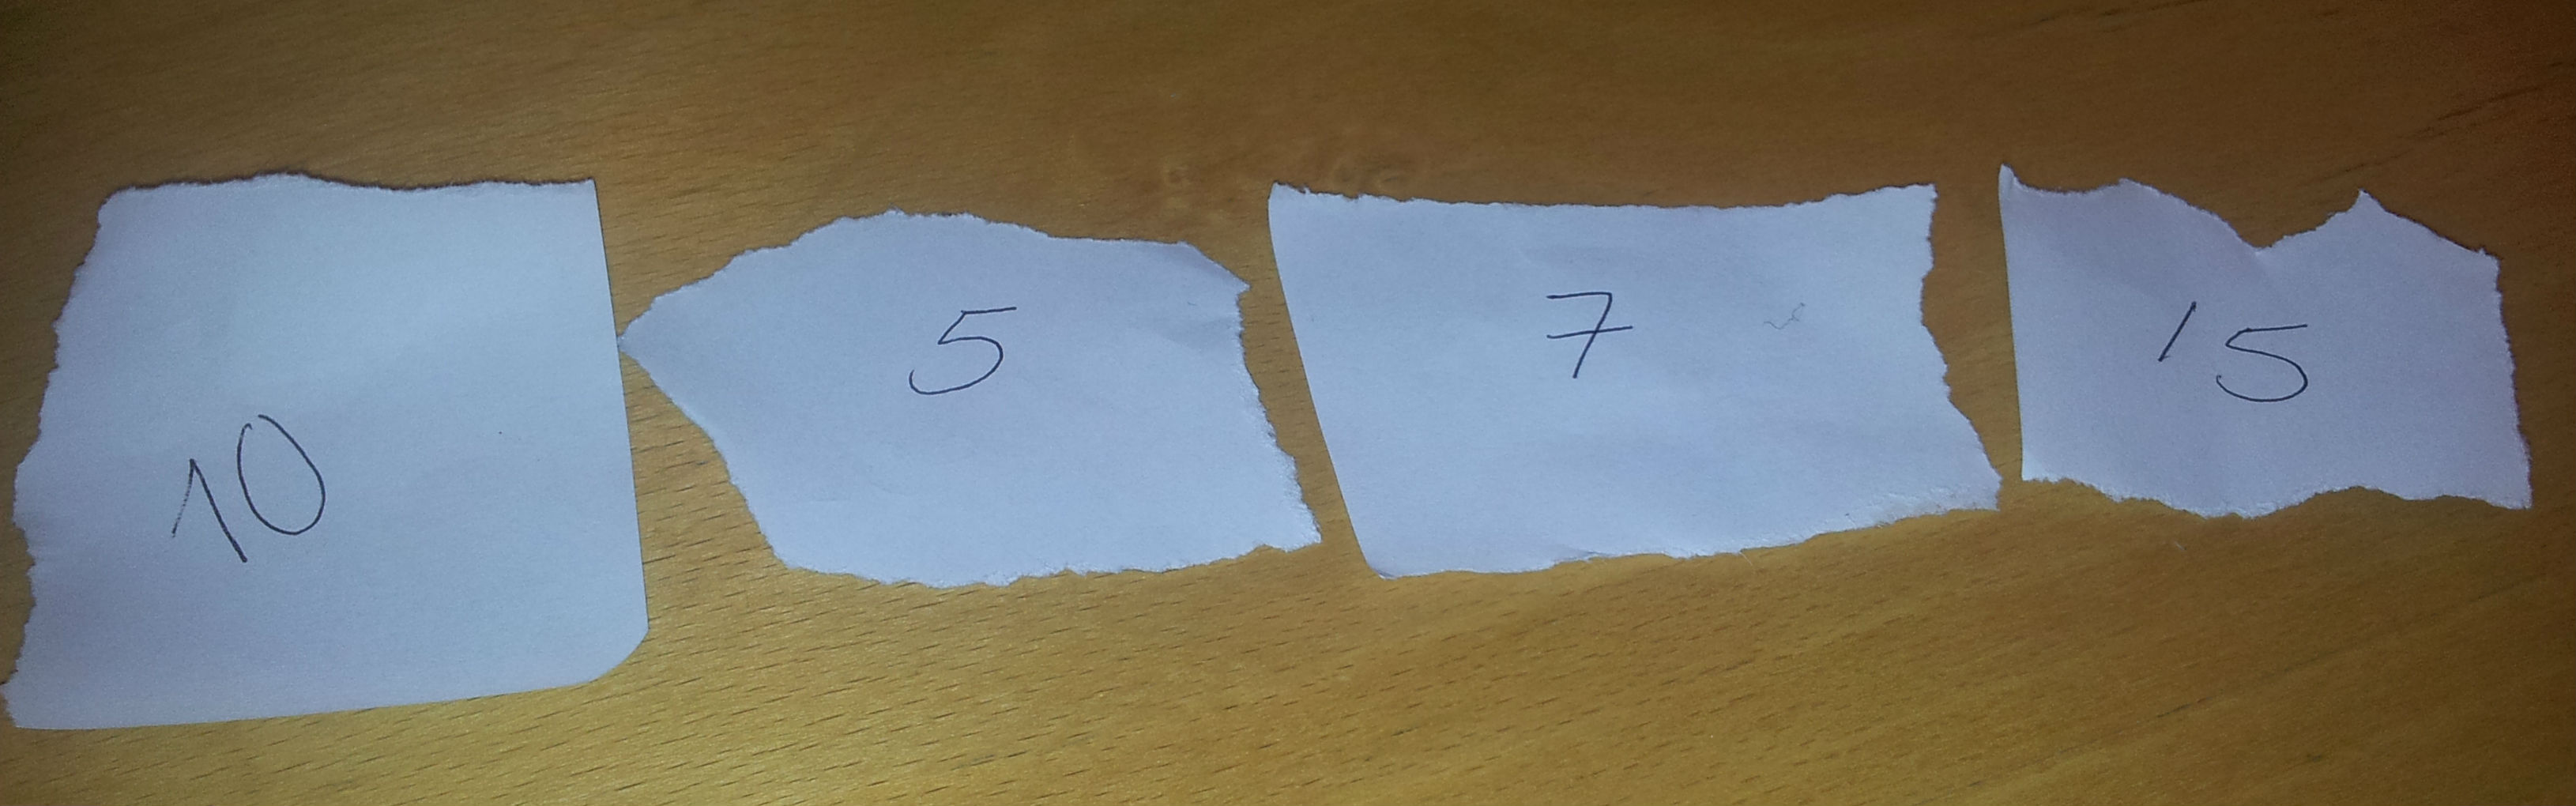
\includegraphics[width=1.0\textwidth]{pictures/estimation.jpg}
		\caption{Hour estimation from sprint 2}
	\end{figure}

	In the start of every sprint, the group performed hour estimation for the sprint.
	Before the hour estimation, the sprint backlog was planned. For every functional requirement
	in the sprint backlog, every person in the scrum team wrote down a guessed hour estimate
	for the requirement. After showing all the estimates, we chose the average of
	the estimates. The reason for doing it this way was because the group 
	was quite unexperienced with hour estimation. When doing it this way, some team 
	members will overestimate and some will underestimate and the result will often be an estimate 
	that is close to the actual effort. 


\clearpage
\section{Game Architecture}
\subsection{Architectural Drivers}
\clearpage
\subsection{Architectural Tactics}

In this section we will list the most inportant quality attributes as 
well as plan the tactis to ensure that we maintain the quality.

{\bf What is a Quality attribute? }

{\bf What is architectural tactics? }


\subsubsection{Modifiability}



\subsubsection{Performance}

\subsubsection{Usability}

\subsubsection{Testability}


\clearpage
\subsection{Architectural Patterns}

A common architectual pattern for video games, is to use a while loop, that runs for the duration of the game. Often using some timing mechanism to update the game at a steady rate. This pattern has it's drawbacks for purpose of this project. It is designed to redraw the screen every frame. On a mobile platform this would waste battery when no notable change has occured which needs to be redrawn. It can also be demanding on the hardware and can run badly on slower hardware. Therefore this project will be using the Model-View-Controller pattern using the JavaScript library Backbone.

The screen works as the view, and is notified whenever changes occur to the game models. The screen collects these events and schedules a repaint. The repaint does not happen immediately after the screen receives an event, but after a certain time, to prevent unnecessarily large spikes in repaints when a bunch of events happen at the same time, which is likely due to the nature of the game. This delaying of repaints is necessary because repaints are slow.

There are 2 singleton objects in the game. One is an Image Library. This object is responsible for loading and storing the sprites the game will draw to the screen. This will allow us to only read and store each sprite one time, saving memory and improving performance. The second singleton object is the Object Pool. This object creates game objects, and stores them while they are not placed on the game map. This object will create all the objects when the game loads, so that they do not have to be created later, further improving performance. Both these singletons are commonly used in video games.

\clearpage
\subsection{Architectural Views}
\clearpage
\subsection{Architectural Rationale}

A common architectual pattern for video games, is to use a while loop, that runs for the duration of the game. Often using some timing mechanism to update the game at a steady rate and redraws the game every frame. On a mobile platform redrawing the entire screen every frame would waste battery when no notable change has occured which needs to be redrawn. It can also be demanding on the hardware and can run badly on slower hardware. Therefore this project will be using the Model-View-Controller pattern using the JavaScript library Backbone. The purpose of using MVC is to collect all the changes that has occured, and find out which of them needs to be redrawn. MVC is not often used for modern video games, because it is common that the game needs to be redrawn every frame anyway so using MVC serves no purpose and just creates extra overhead. However for this project the screen will not need to be redrawn 30 to 60 times a second just to accommodate the high quality 3D idle animations of the game characters.


\newpage
\section{Test Plan}
intro

meets the requirements that guided its design and development,
works as expected,
can be implemented with the same characteristics,
and satisfies the needs of stakeholders
\section{Test Methods}

\paragraph{Black box testing}

Black box testing examines that the functionality of the application works according to the requirements. To carry out a black box test knowledge of internal structure of the application is not necessary. Knowledge of what the application is supposed to do is required, but no how it does it. Hence the software is viewed as a black box, where you can not see the inside, but where input is tested against output to see if the application acts as expected. The strong point of black box testing is detecting unimplemented parts of the specification or missing requirements.

\paragraph{White box testing}

White box testing on the other hand examines the internal structure of the application. In the case of white box testing the tester needs knowledge of \emph{how} the application does what it is supposed to do as well as knowledge about programming. The strong point of white box testing is its ability to uncover errors or problems, and where they are located. Black box testing can detect errors as well, but it can be harder to locate the origin of the errors.

Below, different methods of testing are described briefly.

\begin{description}
  \item[Unit Test] Individual units of source code are tested independently for correctness.
  \item[Functional Test] A system is tested by feeding it input and examining the output against the requirements.
  \item[Usability Test] Examining the products ease of use by testing it on users.
  \item[Compatibility Test] Evaluating the products compatibility with other system software etc.
  \item[Integration Test] Individual software modules are combined and tested as a group.
  \item[Performance Testing] Determine how the system performs in terms of the performance requirements.
\end{description}
\section{Testing Approach}

\subsection{What will be tested}

	Unit testing is a form of white box testing and is a very important part of every software development project. If a unit test fails it is relatively easy to detect the error, and they can be detected early in process. If, or rather when, code is changed, the impact the change has on other parts of the code can easily be determined through unit testing. Due to the limited resources the group possesses in both time and people, unit tests will only be written if there is time. 

	The main focus will lie on functionality testing. Functionality testing is a type of black box testing and it will be performed on an iPhone and an Android phone running the game app.

	Usability testing will also be an important part of the project, considering that if users find the application difficult to use or hard to understand, they can very well decide not to use it, as there are thousands of other games out there.

	During one of the last sprints a compatibility test will be carried out to get an overview of how the application looks on different smart phones.

\subsubsection{What will not be tested}

	Integration testing: Because the application does not use servers or databases, an integration test would be superfluous. Testing of the application as a whole will be done through the various functional tests.

\clearpage

intro

meets the requirements that guided its design and development,
works as expected,
can be implemented with the same characteristics,
and satisfies the needs of stakeholders

\subsection{Test Methods}

\paragraph{Black box testing}

Black box testing examines that the functionality of the application works according to the requirements. To carry out a black box test knowledge of internal structure of the application is not neccessary. Knowledge of what the application is supposed to do is required, but no how it does it. Hence the software is viewed as a black box, where you can not see the inside, but where input is tested against output to see if the application acts as expected. The strong point of black box testing is detecting unimplemented parts of the specification or missing requirements.

\paragraph{White box testing}

White box testing on the other hand examines the internal structure of the application. In the case of white box testing the tester needs knowledge of \emph{how} the application does what it is supposed to do as well as knowledge about programming. The strong point of white box testing is its ability to uncover errors or problems, and were they are located. Black box testing can detect errors as well, but it can be harder to locate the origin of the errors.

\begin{description}
  \item[Unit Test] The first item
  \item[Integration Test] The second item
  \item[System Test] The third etc
  \item[Usability Test]
  \item[Acceptance Test]
\end{description}


\subsection{Testing Approach}

\subsubsection{What will be tested}

Unit testing is a very important part of every software development project. If a unit test fails it is relatively easy to detect the error, and they can be detected early in process. If, or rather when, code is changed, the impact the change has on other parts of the code can easily be determined through unit testing. Due to the limited resources
the group possesses in both time and people, unit tests will only be written if there is time. 

The main focus will lie on functionality testing. Functionality testing is a type of black box testing and it will be performed on an iPhone and an Android phone running the game app.

Usability testing will also be an imortant part of the project, considering that if users find the app diffucult to use or hard to understand, they can well decide not to use it, as there are thousands of other games out there.

A user acceptance test will be performed at the end of the project to let the customer test the final product and
approve or disapprove it.

\subsubsection{What will not be tested}


Integration testing: Because the application does not use servers or databases, an integration test would be superfluous. Testing of the application as a whole will be done through the various functional tests.

Performance testing: Tests if the system working according to the performance demands from the customer. YESNO??????

\subsection{Test Case Overview}

Test cases have been developed for the testing of the fuction of the application. Each test case has been given an identification FT-XX, where FT stands for Functional Test and XX is the number of the test.

Below is the template for the test cases.

\begin{table}[H]
\centering
	\begin{tabular}{ l | p{8cm} }
		\hline
		{\bf Item} & {\bf Description} \\ \hline
		Name & The name of the test \\ 
		Test Id & Identifier of the test \\ 
		Feature to be tested & States the functionality to be tested \\ 
		Requirement & The corresponding requirements that are tested \\ 
		Pre-conditions & Conditions that are fulfilled and can be assumed is working before the test is executed. \\ 
		Steps of Execution & The steps of how the test is to be carried out. \\ 
		Expected result & The expected outcomes of the steps carried out above. \\ 
	\end{tabular}
	\caption{Test case template}
\end{table}

\subsection{Test Cases}

\begin{table}[H]
\centering
	\begin{tabular}{ l | p{8cm} }
		\hline
		{\bf Item} & {\bf Description} \\ \hline
		Name & Map navigation \\ 
		Test Id & FT-01 \\ 
		Feature to be tested & That user should be able to see a small part of the game map and be able to navigate around it.\\ 
		Requirement & FR6.1 and FR6.2 \\ 
		Pre-conditions & None \\ 
		Steps of Execution & 1. Drag a finger over the screen. \\
		& 2. Try to navigate outside the game map. \\
		Expected result & 1. The screen will move across the map in the opposite direction of the finger.\\ 
		& 2. Nothing happens. \\
	\end{tabular}
	\caption{Functional test 1}
\end{table}

\begin{table}[H]
\centering
	\begin{tabular}{ l | p{8cm} }
		\hline
		{\bf Item} & {\bf Description} \\ \hline
		Name & Appearance of buildings \\ 
		Test Id & FT-02 \\ 
		Feature to be tested & That buildings appear around the map at arbitrary intervals and locations. \\ 
		Requirement & FR2.1 \\ 
		Pre-conditions & FT-01 \\ 
		Steps of Execution & 1. Observe that buildings appear around the map at arbitrary intervals and locations.\\ 
		Expected result & 1. Buildings appear around the map at arbitrary intervals and locations at a satisfying rate.\\ 
	\end{tabular}
	\caption{Functional test 2}
\end{table}

\begin{table}[H]
\centering
	\begin{tabular}{ l | p{8cm} }
		\hline
		{\bf Item} & {\bf Description} \\ \hline
		Name & Zooming \\ 
		Test Id & FT-03 \\ 
		Feature to be tested & The shifting between zoomed-out and zoomed-in screens. \\ 
		Requirement & FR6.4 \\ 
		Pre-conditions & FT-01 \\ 
		Steps of Execution & 1. Double tap the screen in zoomed-in mode.\\ 
		& 2. Double tap the screen in zoomed-out mode. \\
		Expected result & 1. The screen will show the whole game map. \\
		& 2. The game will show the part of the game map where the player tapped the screen. \\
	\end{tabular}
	\caption{Functional test 3}
\end{table}

\begin{table}[H]
\centering
	\begin{tabular}{ l | p{8cm} }
		\hline
		{\bf Item} & {\bf Description} \\ \hline
		Name & Main Menu \\ 
		Test Id & FT-04 \\ 
		Feature to be tested & That the buttons in the main menu directs to the correct pages. \\ 
		Requirement & FR1.1, ?Highscore?, ?Start Game? \\ 
		Pre-conditions & FT-01 \\ 
		Steps of Execution & 1. Tap the 'New Game' button. \\
		& 2. Tap the 'Instructions' button. \\
		& 3. Tap the 'Highscore' button. \\
		Expected result & 1. A new game is started. \\
		& 2. The page showing the game instructions is shown. \\
		& 3. The page showing the high score is shown. \\
	\end{tabular}
	\caption{Functional test 4}
\end{table}

\begin{table}[H]
\centering
	\begin{tabular}{ l | p{8cm} }
		\hline
		{\bf Item} & {\bf Description} \\ \hline
		Name & Build Power Plants \\ 
		Test Id & FT-05 \\ 
		Feature to be tested & That it is possible to buy and place power plants on the game map. \\ 
		Requirement & FR2.2 \\ 
		Pre-conditions & FT-01. First the player can afford a Power Plant, subsequently the player can not afford a Power Plant. \\
		Steps of Execution & 1. Drag the build menu into view. \\ 
		& 2. Tap the power plant icon. \\
		& 3. Tap somewhere on the map where a power plant can not be placed e.g. a building. \\
		& 4. Tap an emty area on the map. \\
		& 5. Tap 'OK'. \\
		& 6. Repeat, but tap 'Cancel'. \\
		Expected result & 2.1 If player has enough money the game is set to building mode. \\
		& 2.2 If player does not have enough money, information is displayed. \\
		& 3. Nothing happens. \\ 
		& 4. The player is aksed to either buy or cancel. \\
		& 5. The power plant is placed on the indicated spot and the players amount of money is reduced. \\
		& 6. Leave building mode. \\
	\end{tabular}
	\caption{Functional test 5}
\end{table}

\begin{table}[H]
\centering
	\begin{tabular}{ l | p{8cm} }
		\hline
		{\bf Item} & {\bf Description} \\ \hline
		Name & Build Power Lines \\ 
		Test Id & FT-06 \\ 
		Feature to be tested &  That it is possible to buy power cables and connect buildings and power plants. Proportional COST!! \\ 
		Requirement & FR2.3, FR2.4, FR5.3 \\ 
		Pre-conditions & FT-01 \\ 
		Steps of Execution & \\ 
		Expected result & \\ 
	\end{tabular}
	\caption{Functional test 6}
\end{table}















\begin{table}[H]
\centering
	\begin{tabular}{ l | p{8cm} }
		\hline
		{\bf Item} & {\bf Description} \\ \hline
		Name & Exit Game \\ 
		Test Id & FT-02 \\ 
		Feature to be tested & Test that the game is paused when exiting the game. \\ 
		Requirement & FR1.2 \\ 
		Pre-conditions & \\ 
		Steps of Execution & 1. Leave the game by tapping the home button on the phone. \\
		& 2. Open the game app. \\
		& 3. Tap 'Load Game'. \\
		Expected result & 3. The game is paused at the point where it was left. \\  
	\end{tabular}
	\caption{Functional test 2}
\end{table}

\begin{table}[H]
\centering
	\begin{tabular}{ l | p{8cm} }
		\hline
		{\bf Item} & {\bf Description} \\ \hline
		Name & Upgrade Power Plant\\ 
		Test Id & FT-07 \\ 
		Feature to be tested & That it is possible to upgrade a power plant. \\ 
		Requirement & FR2.5, FR6.3 \\ 
		Pre-conditions & First the player does not have enough money. Subsequently the player does have enough money. \\ 
		Steps of Execution & 1. Tap a power plant. \\ 
		& 2. Choose 'Upgrade Power Plant'. \\
		& 3. Choose "Upgrade" from the pop up. \\
		Expected result & 1. An information box about the cost of upgrading and the effects of upgrading is displayed. \\
		& 2. The system asks whether to 'Upgrade' or 'Cancel'. \\
		& 3. When not having enough money the system gives accordant feedback. \\
		& 3. When having enough money the system upgrades the power plant. \\
	\end{tabular}
	\caption{Functional test 7}
\end{table}

\begin{table}[H]
\centering
	\begin{tabular}{ l | p{8cm} }
		\hline
		{\bf Item} & {\bf Description} \\ \hline
		Name & Enter next level \\ 
		Test Id & FT-09 \\ 
		Feature to be tested & That when one completes a level one is able to continue to the next level. \\ 
		Requirement & FR4.1 \\ 
		Pre-conditions & \\ 
		Steps of Execution & \\ 
		Expected result & \\ 
	\end{tabular}
	\caption{Functional test 9}
\end{table}

\begin{table}[H]
\centering
	\begin{tabular}{ l | p{8cm} }
		\hline
		{\bf Item} & {\bf Description} \\ \hline
		Name & Health Score and Game Over \\ 
		Test Id & FT-10 \\ 
		Feature to be tested & That the game is over when the health score reaches zero. \\ 
		Requirement & FR3.6, FR4.2, FR4.3 \\ 
		Pre-conditions & \\ 
		Steps of Execution & 1. Let several buildings not get power. \\ 
		& 2. Let the health score decrease to zero. \\
		& 3. Tap "Start new game". \\
		& 4. Tap "Back to main menu". \\
		Expected result & 1. The health score is decreasing and houses not supplied are red. \\
		& 2. The "Game Over" page is displayed. \\
		& 3. A new game is started. \\
		& 4. The main menu page is displayed. \\
	\end{tabular}
	\caption{Functional test 10}
\end{table}

\begin{table}[H]
\centering
	\begin{tabular}{ l | p{8cm} }
		\hline
		{\bf Item} & {\bf Description} \\ \hline
		Name & Collect money \\ 
		Test Id & FT-12 \\ 
		Feature to be tested & That it is possible to collect money from buildings connected to the power plants at regular intervals. \\
		Requirement & FR5.1 \\ 
		Pre-conditions & A building is ready to pay for power. \\ 
		Steps of Execution & 1. Tap the building. \\ 
		Expected result & 0. The building has a collect money sign. \\
		& 1. The players money is updated and the sign disappears. \\
	\end{tabular}
	\caption{Functional test 12}
\end{table}

\begin{table}[H]
\centering
	\begin{tabular}{ l | p{8cm} }
		\hline
		{\bf Item} & {\bf Description} \\ \hline
		Name & Tilting \\ 
		Test Id & FT-16 \\ 
		Feature to be tested & That the screen picture is not tiltet when the phone is tilted. \\ 
		Requirement & ??? \\ 
		Pre-conditions & \\ 
		Steps of Execution & 1. Tilt the phone. \\ 
		Expected result & The screen picture stays in place. \\ 
	\end{tabular}
	\caption{Functional test 16}
\end{table}

\subsection{Test Plan Schedule}

This section outlines the schedule of which sprints the test cases were executed, as seen in table XX. Some of the tests were executed in several sprints. The schedule shows the first sprint in which the test was performed. The results of the tests are avaiable in the Test section of each sprint.

\definecolor{lightgray}{gray}{0.9}

\begin{tabular}{| l | l | l |}
	\hline
	\rowcolor{lightgray}
	{\bf Test Case} & {\bf Sprint} \\ \hline
	FT-01 & \\ \hline
	FT-02 & \\ \hline
	FT-03 & \\ \hline
	FT-04 & \\ \hline
	FT-05 & \\ \hline
	FT-06 & \\ \hline
	FT-07 & \\ \hline
	FT-08 & \\ \hline
	FT-09 & \\ \hline
	FT-10 & \\ \hline
	FT-11 & \\ \hline
	FT-12 & \\ \hline
	FT-13 & \\ \hline
	FT-14 & \\ \hline
	FT-15 & \\ \hline
	FT-16 & \\ \hline
	FT-17 & \\ \hline
	FT-18 & \\ \hline
	FT-19 & \\ \hline
	FT-20 & \\
	\hline
\end{tabular}
\clearpage
\subsection*{Test Plan Schedule}

This section outlines the schedule of which sprints the functional tests were executed, as seen in Table \ref{table:testschedule}. Some of the tests were executed in several sprints. The schedule shows the first sprint in which the test was performed. The results of the tests are avaiable in the Testing section of each sprint.

\definecolor{lightgray}{gray}{0.6}

\begin{table}[h]
\centering
\begin{tabular}{| l | l || l | l |}
	\rowcolor{lightgray}
	\hline
	{\bf Test Case} & {\bf Sprint} & {\bf Test Case} & {\bf Sprint} \\ \hline
	FT-01 & Sprint 1 & FT-16 & Sprint 3 \\ \hline
	FT-02 & Sprint 1 & FT-17 & Sprint 3 \\ \hline
	FT-03 & Sprint 1 & FT-18 & Sprint 3 \\ \hline
	FT-04 & Sprint 2 & FT-19 & Sprint 3	\\ \hline
	FT-05 & Sprint 2 & FT-20 & Sprint 3 \\ \hline
	FT-06 & Sprint 2 & FT-21 & Sprint 3 \\ \hline
	FT-07 & Sprint 2 & FT-22 & Sprint 3	\\ \hline
	FT-08 & Sprint 2 & FT-23 & Sprint 3 \\ \hline
	FT-09 & Sprint 2 & FT-24 & Sprint 3 \\ \hline
	FT-10 & Sprint 2 & FT-25 & Sprint 4 \\ \hline
	FT-11 & Sprint 2 & FT-26 & Sprint 4 \\ \hline
	FT-12 & Sprint 2 & FT-27 & Sprint 4 \\ \hline 
	FT-13 & Sprint 2 & FT-28 & Sprint 4 \\ \hline
	FT-14 & Sprint 3 & FT-29 & Not implemented. \\ \hline
	FT-15 & Sprint 3 & FT-30 & Not implemented. \\ \hline
\end{tabular}
\caption{Testing Schedule}
\label{table:testschedule}
\end{table}
\clearpage
\section{Usability Testing}

	A usability test will be performed in sprint 3 to examine how well actual users interact with the game, and	discover errors and areas of improvement. First we have a look at what usability is.

\subsection{What is Usability}

	Usability can be defined as:

	\begin{quote}
	The effectiveness, efficiency, and satisfaction with which specified users 
	achieve specified goals in particular environments. (ISO 9241-11) \cite{ISOusability}
	\end{quote}

	\paragraph{Effectiveness}

		The easiest way to measure effectiveness is as the number of tasks completed without assistance. Effectiveness provides a quantitative measure of the degree to which users are able to perform the tasks that the product will offer. It can be measures as the number of tasks the user was able to perform on their own in a usability test. Problems experienced by the user will also be reported, because it tells us about aspects with the user interface that reduced applicability.

		Measuring effectiveness will be important to our product because the users of the game will not get any training in how the game works, they need to work this out on their own by reading the game instruction and trying the game. If they find it hard to perform the tasks in the game, they will probably not return to play it.

	\paragraph{Efficiency}

		Efficiency is about the resources used or time spent to carry out a task. It can be measured as "time spent per task".
		By measuring how long each task will take you get an idea of the system's efficiency.

		It is important to us to find out if users can perform basic game tasks efficiently. Because if basic tasks, that is to be performed over and over again, are intakes long time to carry out, the game experience will deteriorate.

	\paragraph{Satisfaction}

		Subjective satisfaction says something about the user's subjective experience and assessment of the product. Satisfaction can be measured both quantitatively and qualitatively. The system usability scale (SUS) is a form of quantitative measure, where users rate various aspects of the product on a scale from 1 to 5. Qualitatively subjective satisfaction can be measured by interviewing the subjects after the test. Much can also be interpreted on the basis of what they say during the test. It is important to have some qualitative measure in addition to the quantitative, because the questions in the SUS form is general and may not cover all aspects of our product.

		This is important to get insight into the opinions the user has about the product. What is working, what is not working and what could be improved.

	\paragraph{Specified users in particular environments}

		It is important to identify relevant user groups, and make sure that the testers is representative of the user groups. If the system is to be used in a particular environment, and if possible, this environment should be tried recreated, for the test. In our case, the environment is not of great importance, as the game can be played practically anywhere a mobile phone can be.

\subsection{Planning the Usability Test}
\label{subsec:planustest}

	\paragraph{Who are the players?}\mbox{}\\

		The target group for this product is people that own a smart phone and have an interest in apps and playing games.We also hope to reach people who are the ones paying for the electricity in their household. 

	\paragraph{How many players will be invited?}\mbox{}\\

		Research shows that with 15 testers the number of usability problems found reaches 100\%. \cite{numberOfUsers} It also shows that with more than 5 testers one learns less and less when introducing additional testers. The usability test will mainly be qualitative and focus on obtaining insight into the design of the game and what could be improved. The quantitative aspect of the test will come second and be obtained through a usability survey. In a quantitative study it is desirable to have more than 5 testers, but taking into account the little time we have at hand, we feel 5 players will be sufficient for this usability test.

	\paragraph{How will players be recruited?}\mbox{}\\

		Players will be recruited by asking students at the computer lab if they want to take part in a usability test. We are aware that this will lead to a very homogeneous test base, but the focus of the test is not to examine whether the game appeals to all members of the target group. The testers will be people that do play games on their own phones and that have a lot of experience with mobile apps, therefore we hope they will have strong opinions and ideas for how a good game should be.

	\paragraph{What should be tested?}\mbox{}\\

		We want to examine if people understand the concept of the game, how to play it, the goal of the game, 
		and how not to lose. Is it intuitive for the player to understand how one earns money? From the process 
		of building power plants, serving buildings and collecting money. Is it intuitive how one keeps 
		the health bar from decreasing? That is by serving all the houses with power.

		We want to discover issues, problems, errors, vaguenesses, missing functionality and other areas 
		of improvement. We want to inquire whether the testers find the game fun to play, or if it could 
		be more fun with certain improvements.

		The player will not be given instructions or scenarios explaining what to do, because we want 
		the player to find things out for himself, just like it would be if the player had just 
		downloaded the app. We want to examine if the player manages to play the game without being 
		told how to play, beyond a small introduction and the information the game instructions provide. 

	\paragraph{How will the test be executed?}\mbox{}\\

		The player will get a brief oral explanation of the elements and goal of the game, 
		and can chose to read the game instructions that are found in the game menu.

		The player will then start a new game and will be encouraged to think aloud. 

		These thoughts may regard:

		\begin{itemize}
		  \item Explanations to why certain actions are chosen, the first time they're executed.
		  \item What they see on the game screen and what they think it means.
		  \item Problems that arises. For example "I want to be able to ..., but don't know how to do it". 
		  \item Bugs or errors that occur.
		  \item What was difficult to achieve.
		\end{itemize}

	\paragraph{Observation form}\mbox{}\\

		During the execution of the test one of the team members is the observer, and will document all problems, bugs or errors the player encounters. The observer reports what the problem is, what causes the problem and what might be a possible solution to the problem. The observation form can be found in Appendix \ref{chap:observationform}.

	\paragraph{Follow-up questions}\mbox{}\\

		After the player has played the game, a small interview will take place, where the player is presented with potential questions the observator has found during the test, as well as three pre-made questions. The player will also be encouraged to give feedback on matters, he or she felt the questions did not cover.

		1. Do you have any specific complaints about the game?

		2. Do you have any suggestions that you feel would make the game better?

		3. Was there something that was good or that you liked about the game?

	\paragraph{Usability Survey}\mbox{}\\

		Finally the player will be asked to fill out a survey, where he or she is asked to rate certain aspects of the game on a scale from 1 to 5. There are in all 18 questions. The first 8 questions are inspired by the System Usability Scale \cite{sus} and adapted to our problem, whereas the 10 following questions are inspired by a question form that is more specific to games \cite{evaluationSheet}, and the scale of each question has its own specified rating. The form with the questions can be found in Appendix \ref{chap:appussurvey}.



%Sprint chapters
\clearpage
\section{Planning phase}
	In this section it will be described how the project startet
	and how the project was defined with scope and requirements.

\subsection{Getting to know each other and the customer}
	

\subsection{Project Assignment}
	Sette oss inn i oppgaven og hva kunden ville ha
	Project scope

\subsection{Define the Project Scope}

\subsection{Preliminary studies and Project Planning}

\subsection{Game Concept Development}
	Utvikling av spillkonsept

\subsection{Specification of the Requirements}

\subsection{Planning the first sprint}

\subsection{Group dynamics}

\subsection{Phase Results}

\clearpage
\section{Sprint 1}
This is the first sprint of this project. In this sprint we will start the implementation
and try to build a fundament in the code so the rest of the implementations will go fast
and smooth. 

\definecolor{gray}{gray}{0.6}

\subsection{Sprint Planning}
	The group planned a small delivery in this sprint, because we need time to set up the development environment and gain knowledge about the backbone framework and javascript, to make the implementations in the following sprints easier. During the sprint we will have the basis for the implementation ready such as models, views and presenters. The functional requirements concerning the map navigation and zooming are also to be implemented.

	In order to start implementing the other functional requirements, it requires that we have the map to put them on, and that all the elements in the game such as building, power plant and power line have been defined and implemented 

	To be able to keep up the testing activity in the upcoming sprints, we will try to get started with unit tests. This will probably take some time since testing is a new concept to many in the group as well as Jasmine is a new framework for all in the group. 

\subsection{Duration and Workload}
	When the group had the firs meeting, we agreed to have sprints lasting for 2 weeks.
	After the 10 days into the first sprint, the group realized that goal was not reachable.
	The group decided to change the first sprint duration to 3 weeks instead of 2 weeks. \\

	{\bf Duration:} 09.09 - 29.09 (3 weeks)\\
	{\bf Workload:} This is the list with hours spent (the whole group) on the project in this sprint.
	\begin{itemize}
		\item {\bf Planning:} 11 hours
		\item {\bf Development:} 94,5 hours
		\item {\bf Design:} 14 hours
		\item {\bf Documentation (report):} 40,5 hours
		\item {\bf Testing:} 1 hour
	\end{itemize}
	{\bf Total workload: } 161 hours \\
	
	The group's goal was to work at least 20-25 hours pr/person every week. We did not manage this at this sprint, but we had a average of 13,5 hours/week (161 hours/4 persons/3 weeks = 13.5 hours). 
	In section 'problems during the sprint', we have written what have happened during this sprint.
	Many of the scenarios from that section affected the workload on the group. 

\subsection{Sprint Backlog}

	Table \ref{table:backlogsprint1} shows the backlog for what is planned to be delivered at the end of this sprint.
	Total estimation is: 83 hours

\begin{table}[H]
\begin{tabular}{| p{1cm} | p{7cm} | p{2cm} | p{2cm} |}
	\hline
	\rowcolor{gray}
	ID & Description & Estimate & Actual effort \\ \hline
	FR2.1 & Buildings should appear around the map at arbitrary intervals and locations. 
	& 11 hours & 10 hours \\ \hline
	FR6.1 & The user should be able to see a small part of the game map. 
	& 20 hours & 21.5 hours \\ \hline
	FR6.2 & The user should be able to navigate around the map using the touch function on the phone 
	& 29 hours & 27 hours \\ \hline
	FR6.4 & The user should be able to view all of the map by double tapping the screen; double tapping a point on the complete map should zoom in on that area. 
	& 33 hours & 36 hours \\ \hline
\end{tabular}
\caption{Sprint backlog sprint}
\label{table:backlogsprint1}
\end{table}

\subsection{Implementation}

\subsubsection*{Models}
	We have been using Backbone to implement the game models in this project. In Sprint 1 we have implemented 
	the following models to store game data.
	\begin{itemize}
		\item {\bf Building}
		The building model stores information about the buildings location on the game map as well as a reference 
		to the image that should be drawn on the map.
		\item {\bf Level}
		This model contains the map and player object. It is this object's job to handle the logic responsible for 
		updating the state of the game models.
		\item {\bf Map}
		The map model has two main functions. The first is to hold a Backbone Collection with all the buildings 
		that are placed on the map. The second is to maintain which part of the map that should be painted.
		\item {\bf Player} 
		The player model stores how many lives the player has and how much money the player has available to them.
	\end{itemize}

\subsubsection*{Presenters}
	Backbone Presenters are the JavaScript objects that connects the Backbone Models 
	to the visual HTML code. They listen to changes to the Backbone Models and changes 
	the HTML objects accordingly. The Presenters also handles input events from the HTML objects.
	
	We have implemented the four main states of the game. Each state has its own purpose.
	\begin{itemize}
		\item {\bf Main menu} The main menu where you navigate to the other screens.
		\item {\bf Ingame} THis is where you play the game, the game loop runs 
		and the game state is rendered to the screen.
		\item {\bf Instructions} In the Instruction screen you can read about how to play the game.
		\item {\bf Highscore} This lets you see how well you did while playing the game.
	\end{itemize}
	
	\begin{figure}[H]
	\centering
	\subfigure{
		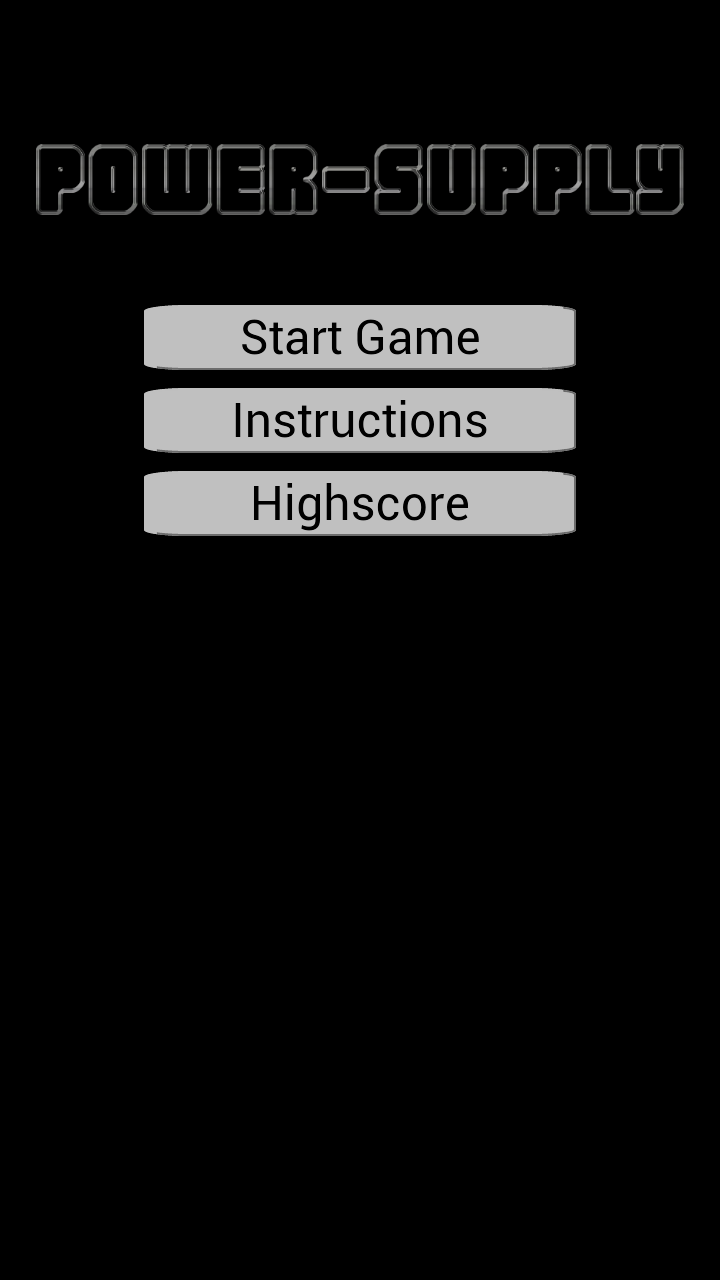
\includegraphics[scale=0.2]{pictures/game_screenshot_2}
	}
	\subfigure{
		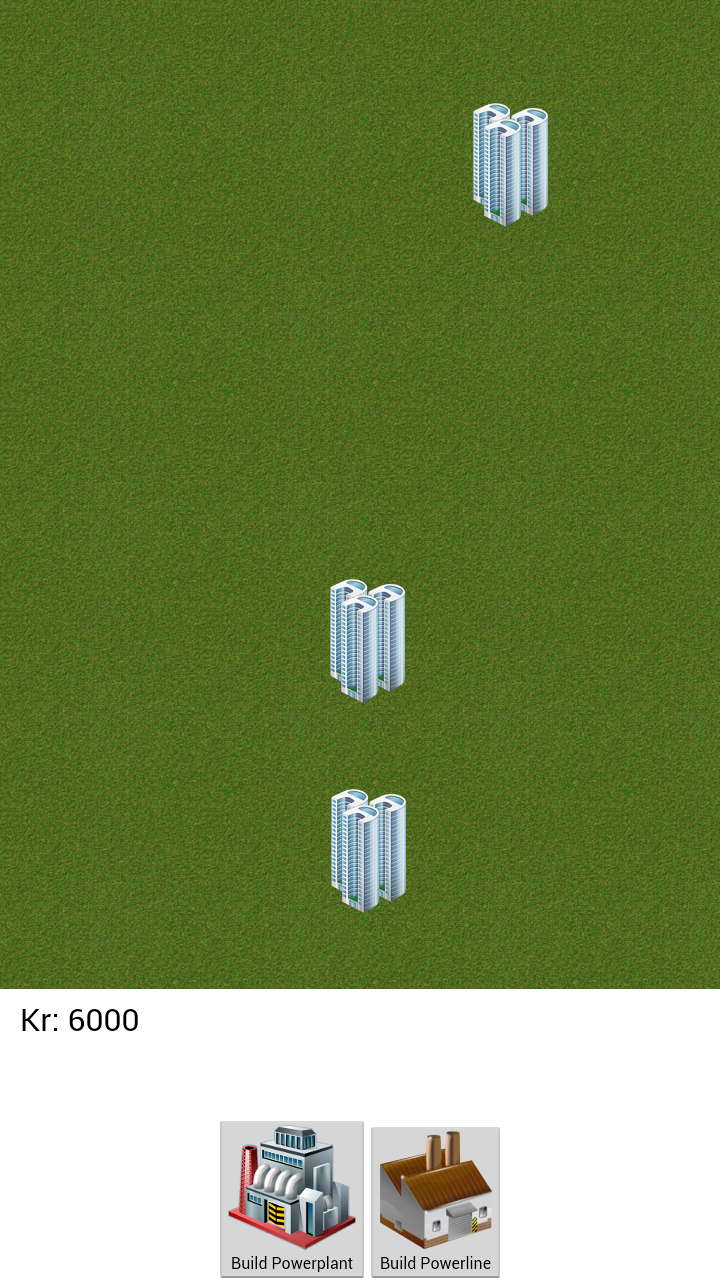
\includegraphics[scale=0.2]{pictures/game_screenshot_1}
	}
	\caption{Home screen and game map from sprint 1}
	\end{figure}

	\subsubsection*{Other Implementations}
		\begin{itemize}
			\item {\bf Place buildings on map} The game will place buildings at random positions on the map.
			\item {\bf Rendering} The state of the map will be rendered to the screen.
			\item {\bf Game Loop} The game loop updates the state of the game continuously.
		\end{itemize}

\subsection{Testing}
	Unit tests were not written in this sprint. Much time has been spent getting to know 
	the programming tools that are to be used and the focus has been on creating a base for further 
	programming as well as something more visual to show the customer. The testing that has been 
	carried out has been functional testing as well as debugging using Android Debug Monitor. Functional 
	testing of the implemented requirements took place at the end of the sprint. The functional tests 
	executed in this sprint are listed in Table \ref{table:testsprint1}.

\definecolor{lightgray}{gray}{0.9}

\begin{table}[H]
\begin{tabular}{| p{3cm} | p{7cm} | p{2cm} |}
	\hline
	\rowcolor{lightgray}
	{\bf Test Case} & {\bf Result} & {\bf Evaluation} \\ \hline
	FT-01 Map navigation & It is possible to move around the map as expected. When trying to move outside the map one stays in place in the outskirts of the map. & Pass. \\ \hline
  	FT-02 Appearance of buildings & Buildings do appear at regular intervals, within the map, but the rate at which they appear needs to be adjusted. It is also possible for a building to appear on top of another. & Still needs some corrections. \\ \hline
	FT-03 Zooming & Zooming is working as expected. When navigating fast the system sometimes interpret it as zooming. & Pass \\ \hline
\end{tabular}
\caption{Performed tests from sprint 1}
\label{table:testsprint1}
\end{table}

\subsection{Group Dynamics}
	In the start of this sprint we had a major problem that many of the group members was ill or 
	that many members didn't have the time to contribute to the project. 
	This is one of the risk factors 
	that we have listed in the risk analysis. 
	Apart form that, we had some problems with the group dynamics. The members in the group are 
	quite different and like to work in different ways. The main problem was 
	that many of the group members
	have different experiences with this kind of group work, technology as well as we have 
	different personalities.
	We managed to solve this problem by sitting down and discussing the problem. We discovered that
	one of the main problems was that the role allocation and the responsibility had not 
	been present.
	After we allocated the roles with a specific responsibility, many of our problems was solved and
	we have been able to work better as a group.

	Sprint 1 was the first phase in the project with implementation and coding. In the start, 
	many in the group had
	some problems with setting up the development environment (specially on windows). We managed
	to solve this problem, but it affected the total implementation because the whole group couldn't 
	contribute as much as we hoped. One solution was to go over from windows to ubuntu. 
	In the end of the sprint, everyone had a working development environment.

	Since no members in the group have a lot experience with the technology, it was sometimes hard
	to be able to do the implementations fast enough, or even know where to start. 
	Hopefully we will not have as much problems in the next sprints, but it is still a risk factor 
	since we are still quite inexperienced with javascript, mobile development and the framworks we use. 

\subsection{Customer Feedback}
	In this sprint we did not get any feedback from the customer. We hope that the customer
	will get more involved in the next sprint. In the next sprint the group would like to have
	more feedback on the requirements. This is crucial because of the chosen working 
	methodology.

\subsection{Sprint Retrospective}
	\subsubsection*{Start doing: } 
		\begin{itemize}
			\item Require that the customer will give us feedback on the
			requirement specification in the next sprint.
			\item When one from the scrum team start implementing on a new feature, 
			it is a good practice to make a own branch in git for that. 
			\item Always pull regularly from the master branch when developing
			on a own feature branch.
			\item Start talking more to the other group members. This is crucial 
			for working together as a team.
		\end{itemize}
	\subsubsection*{Stop doing: } 
		\begin{itemize}
			\item stop coming late to the group appointments.
		\end{itemize} 

\clearpage
\definecolor{gray}{gray}{0.6}
\section{Sprint 2}

\subsection{Sprint Planning}
	In this sprint the group is planning on a big delivery. In the last sprint the group
	implemented the fundamental structure in the game, such as models, presenters and views. 
	The implementations in the last sprint was crucial for this sprint in order to 
	be able to implement a lot of game logic to make the game more "playable".

	The group will focus on the requirements with critical and high priority in order
	to deliver as promised. There should be no critical requirements left at the end of 
	the sprint, and only a few requirements with a high priority. There will also be more 
	focus on the implementation, rather than writing more content to the report.

	At the end of the sprint, we will also use time testing what has been implemented.
	The tests will ensure that the functions that have been implemented works as planned 
	and that the product is ready for the sprint delivery with the customer. The testing is 
	done manually because there will not be time to implement unit tests in this sprint.

	During the sprint, the group members need to focus more on the workload because we did
	not manage to reach the workload expected from the course staff. This is crucial
	for the group in order to be able to deliver the product and meet the deadlines.

\subsection{Duration and workload}
	In the last sprint, we did not reach the workload expected by the course staff.
	In the start of the sprint, the scrum master made timetable together with the
	scrum team in order to ensure more workload. The goal was to at least have an
	average workload pr/person to be 25 hours pr/week. 

	{\bf Duration:} 30.09 - 13.10 (2 weeks)\\
	{\bf Workload:} This is the list with hours spent (the whole group) on the project in this sprint.
	\begin{itemize}
		\item {\bf Planning:} 11 hours
		\item {\bf Development:} 85 hours
		\item {\bf Design:} 0 hours
		\item {\bf Documentation (report):} 65 hours
		\item {\bf Testing:} 3.5 hours
	\end{itemize}
	{\bf Total workload: } 165 hours \\

	The group's goal was to work at least 20-25 hours pr/person every week in this sprint. 
	We did manage the workload, and we had a avrage of 20.6 hours/week (165 hours/4 persons/2 weeks = 20.6 hours). 
	The scrum master have the responsibility to ensure that the workload is met with the
	expectations from the course staff, and we managed it in this sprint.
	The changes from the last sprint is that we worked late hours and used the weekend effective
	since the entire group is occupied with UKA, voluntary work and homework.

\subsection{Sprint backlog}

	In this sprint we planned to implement the most of the requirements with critical and high
	priority. In the start of the sprint we only planned to implement 8 requirement, but
	during the sprint we manage to implement them and added more requirements to the sprint backlog.
	In the end of the sprint the backlog consisted of a total of 15 requirements. Here are the
	sprint backlog from this sprint:

	\begin{tabular}{| p{1cm} | p{8cm} | p{3cm} |}
		\hline
		\rowcolor{gray}
		ID & Description & Estimate \\ \hline
		FR1.1 & The user should be able to read game instructions from the main menu
		& \\ \hline

		FR1.12 & The user should not get the opportunity to tilt the screen by tilting the phone. & \\ \hline
		
		FR2.2 & The user should be able to buy and place several power stations on the game map.
		& \\ \hline

		FR2.3 & The user should be able to buy and place power cables on the map. &  \\ \hline

		FR2.4 & The user should be able to upgrade the power plant. & \\ \hline

		FR2.8 & The user should be able to see information about a buildings when tapping on them.
		& \\ \hline

		FR3.6 & When an existing building is not supplied with power within a certain amount of time, 
		the house should disappear and the player's health score should decrease. & \\ \hline

		FR4.2 & The user should be able to continue a level while the health score is greater than zero. 
		When the health score reaches zero, the game is over. & \\ \hline

		FR5.1 & The user should be able to collect money from the buildings connected to the power plant
		& \\ \hline

		FR5.2 & When connecting buildings through power cables, there should be a cost which is 
		proportional to the length of the cable. & \\ \hline

		FR5.3 & It should cost money to upgrade the power plant. & \\ \hline

		FR6.3 & The user should be able to click on a power plant to receive information about 
		the cost of upgrading it and what the upgrade does. & \\ \hline

		FR6.7 & The user should be able to see the main menu when he or she starts the game. & \\ \hline

		FR6.8 & When the player wants to place a power plant or a power cable in building mode, 
		the player should be prompted if they want to go through with it, or cancel. & \\ \hline

		FR6.9 & The user should be able to see that he or she is in building mode when selecting 
		a building to build in the hub menu. & \\ \hline

		FR6.10 & The user should be able to see that a building has gone without power for 
		some time, and is affecting the player's health score if the building is not connected 
		to a power plant before it disappears. & \\ \hline

	\end{tabular}

\subsection{Implementation}
	
	This is the actual implementation of requirements that we managed to implement
	from the sprint backlog.
	
	\begin{itemize}
		\item {\bf Building mode:} When the player open the hud (menu in the bottom of the screen) and presses
		on the build powerplant/powercable image, the player enters the building state 
		"build powerplant/build powerlines". The game state is set back to normal after the player 
		is finished with the building. The game has a state variable that contains which mode the 
		game is in (Normal, build power plant or build power lines). When the player is in the building
		state, two lines will appear (on top and bottom) on the screen that looks like constructions mode
		(yellow and black stripes). The look and feel is important for the user to understand that
		the game-state is changes to building mode. 

		\item {\bf Upgrade power plants:} When the player taps on the power plant, a pop-up will appear.
		In the pop-up it will show the level the power plant is in and how much it will cost the 
		player to upgrade the power plant. If the player choose to upgrade the power plant the level will
		increase by 1. If the player do not want to upgrade, he or she press "cancel" and the player will be sent
		back to the game. The part that is not implemented here is that when a power plant is upgraded, 
		it will be able to serve more buildings with power and this should also be added to the building 
		information in the pop-up. If the player does not have enough money, the player gets a message 
		that he or she cannot upgrade.

		\item {\bf Building and buy power plants:} When the player open the menu in the bottom and 
		choose the "build powerplant" icon, the player enters the building mode and is able to 
		tap on the screen where he or she wants to place the power plant. When the player taps on the
		location to place the building, it will a appear a pop-up with the question if the player 
		want to buy and build the power plant. If the player want to build the power plant, a certain
		amount of money will be payed from the players money or if the player press "cancel", the 
		game goes out of the building state and back to normal. If the player choose to buy the 
		power plant, but do not have enough money, the player get a message that he or she do not have
		enough money and the game state will be set back to normal. 

		\item {\bf Connect buildings to power plants:} When the player open the menu in the bottom and 
		choose the "build powerline" icon, the player enters the building mode and the player is able
		to build power lines. The power lines is build by tapping on the desired en-points (house-house 
		or house-power plant).

		The part that is not implemented is the logic for handling the "connection state" of a building, 
		as well as the amount of power a power plant can serve. It is not implemented that if the building
		is connected, the countdown will stop and make money that the player can collect. The money should
		only be "produced" if the building is connected to a power plant. The amount of money that is 
		produced should be building specific because different buildings use different amount of power, and
		therefore need to pay a different amount of money. 

		\item {\bf Collect money:} When a building is connected to another building, it starts 
		"producing" money. The building will show a icon of a coin when the player is able to 
		collect the money. The money is collected when the user taps on the building with a coin. 

		The parts that is missing is that it needs to check whether the connected building is a power plant 
		or just another building. It should only produce money if it is connected to a power plant. 
		If the building have produced money, a coin will appear on the building. When the player tap
		on a building with a coin icon, it will collect the money and the players amount of money 
		will increase. 

		\item {\bf Game over:} When the health bar is zero, the game is over and the game over screen 
		is showing. When the player press "ok", the player is sent to the main menu and is able to 
		start a new game. This part may need some changes to the look and feel, but it is working.

		\item {\bf Main menu:} When the game is starting, the app is showing the main menu. 
		From this menu, the player is able to choose between "Start game", "Instructions" and high score.

		\item {\bf Money and goal:} When the player has started the game, the score and goal for
		the level is showing in the hud. To get to the next level, the player need to get the same
		amount of money as the goal in order to go to the next level. The logic for the level
		is not finished yet.

		\item {\bf Information about power plant:} If the user taps on a power plant it will pop up
		information about the power plant like level and upgrade information. It is not implemented yet,
		but it will be implemented more information like how much power it can serve and how mange
		buildings that are connected. 

		\item {\bf Health bar:} In the bottom of the game it is showing a health bar. If the 
		health bar is below zero, it is game over, so the player need to keep track of the health.
		A user loses health if a new buildings countdown is over and the building disappears.
		The health bar will send a signal with a color. If the player has full health bar the bar is
		green, then it gets orange and in the end it is red. 

		\item {\bf Countdown on building:} when a building appear, a countdown starts. If the player
		do not connect the building to a power plant, the countdown wont stop. If the countdown is
		finished, the house will disappear and the health bar will decrease. This is a signal to
		the player so he or she is able to connect the building to a power plant in order to not loose
		health. 

	\end{itemize}

	This is the requirements that was in the sprint backlog that we did not
	manage to finish and have removed to sprint 3:

	\begin{itemize}
		\item {\bf Information about building:}

		\item {\bf The cost of the power lines:}

	\end{itemize}

	\begin{figure}[H]
	\centering
	\subfigure{
		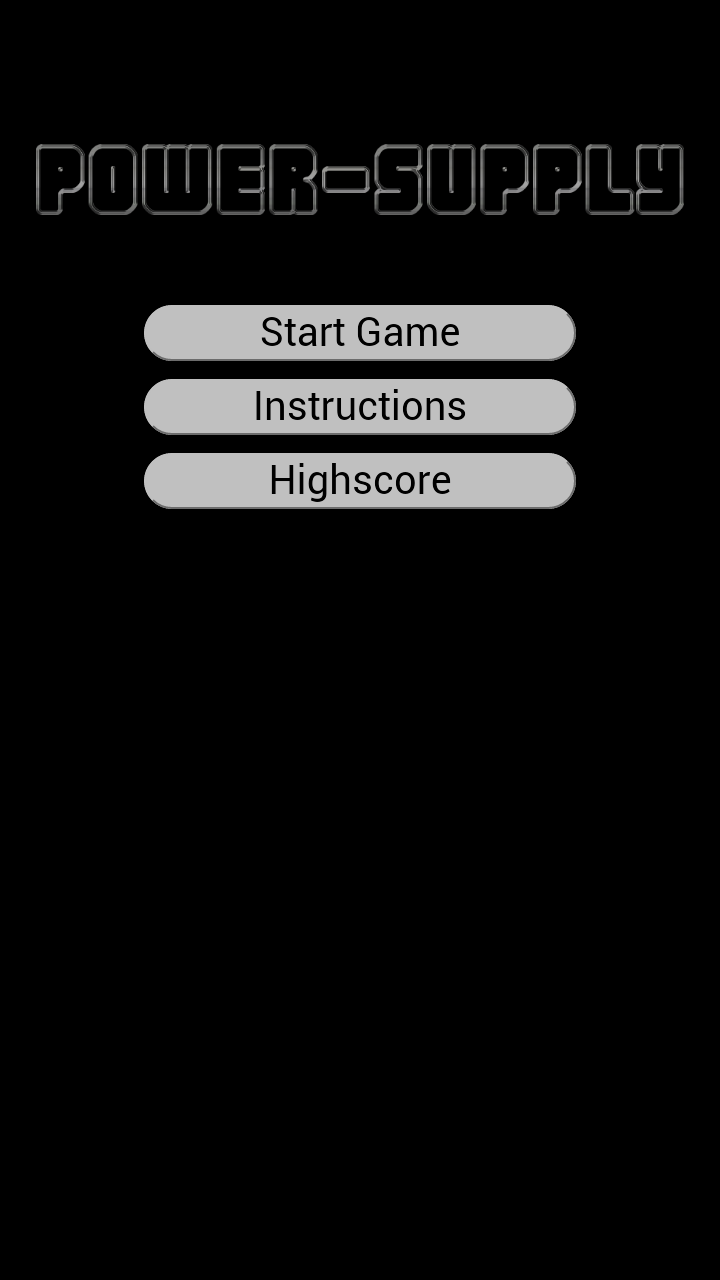
\includegraphics[scale=0.17]{pictures/sprint2-screen/sprint2-2}
	}
	\subfigure{
		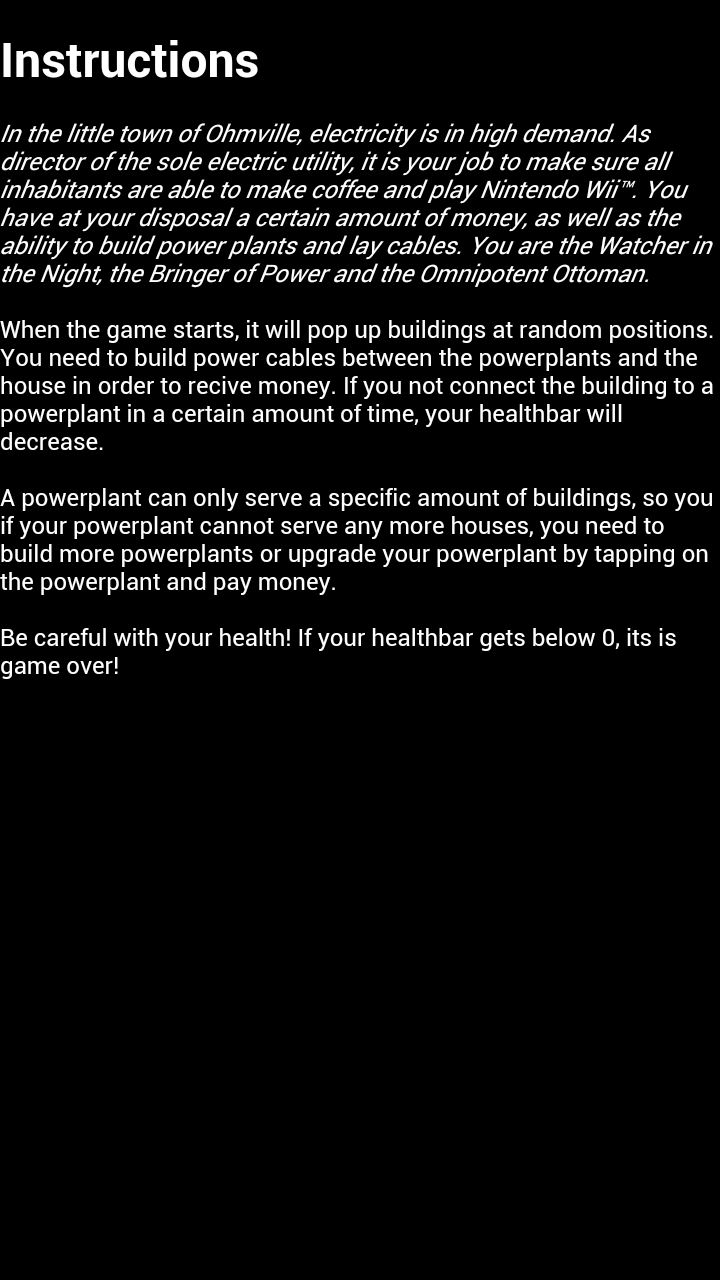
\includegraphics[scale=0.17]{pictures/sprint2-screen/sprint2-3}
	}
	\caption{Main menu and instruction screen}
	\end{figure}

	\begin{figure}[H]
	\centering
	\subfigure{
		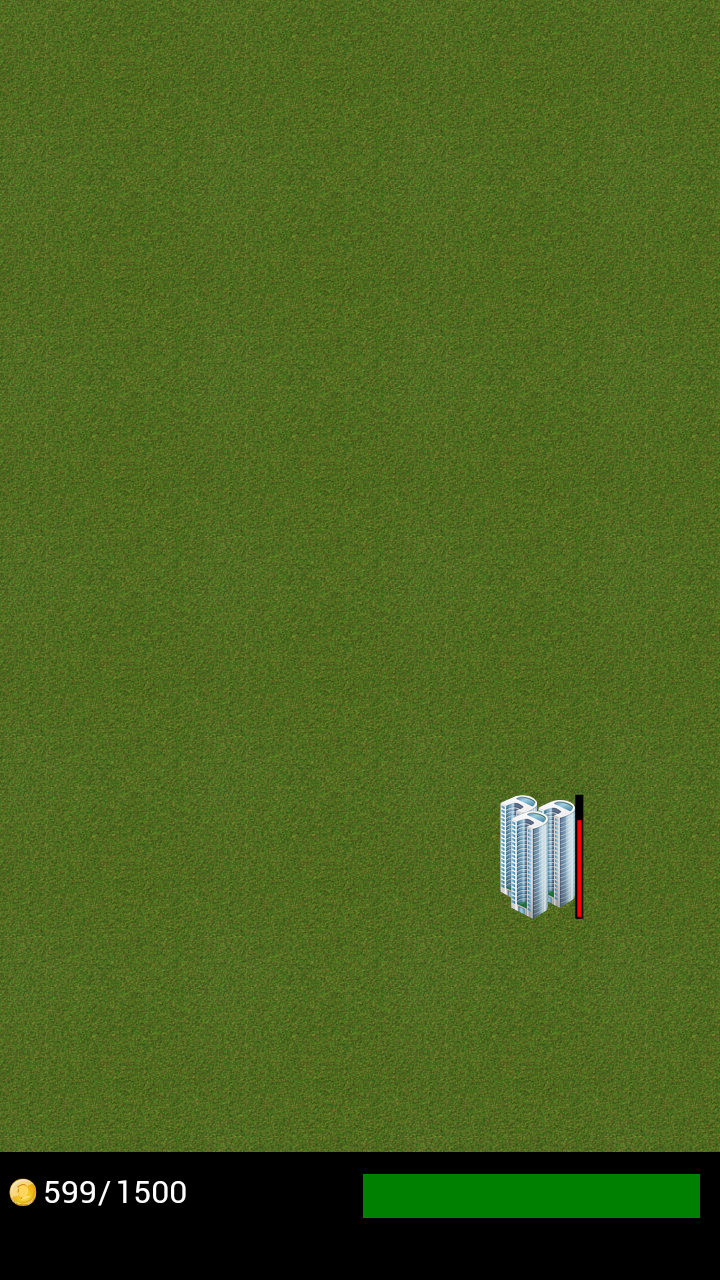
\includegraphics[scale=0.17]{pictures/sprint2-screen/sprint2-4}
	}
	\subfigure{
		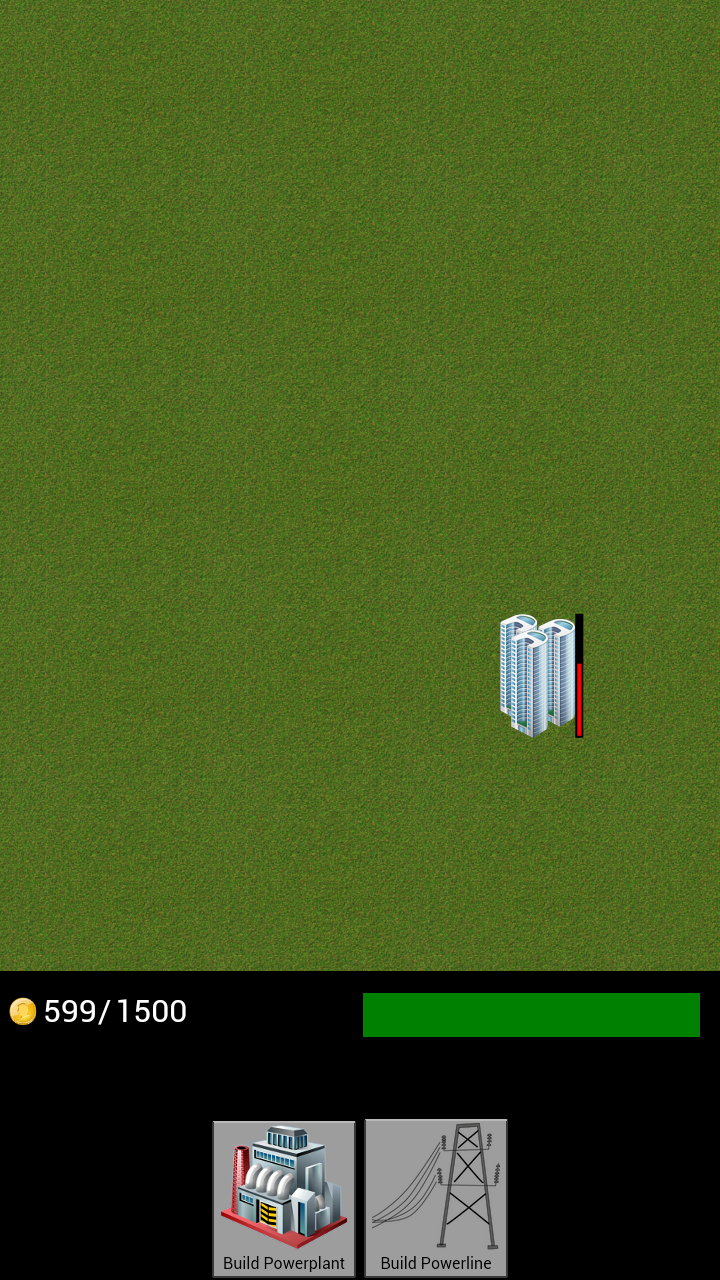
\includegraphics[scale=0.17]{pictures/sprint2-screen/sprint2-5}
	}
	\caption{Ingame headsup display (hud)}
	\end{figure}

		\begin{figure}[H]
	\centering
	\subfigure{
		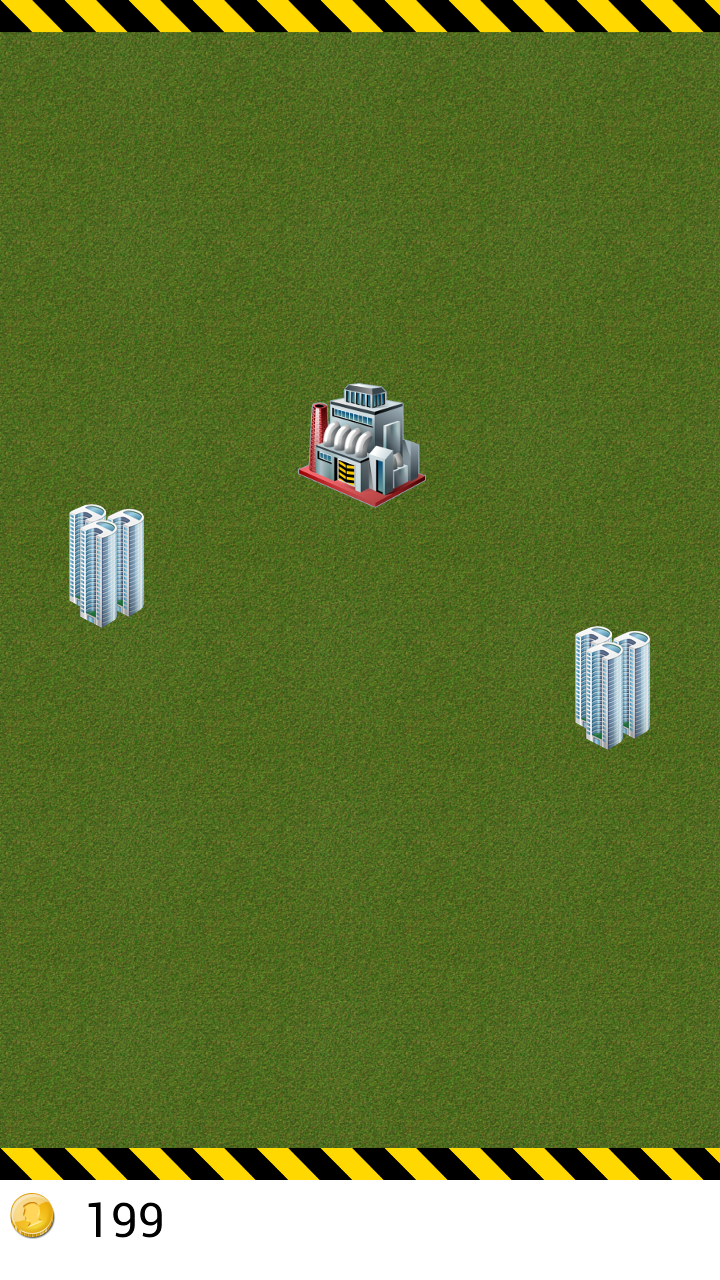
\includegraphics[scale=0.17]{pictures/sprint2-screen/sprint2-1}
	}
	\subfigure{
		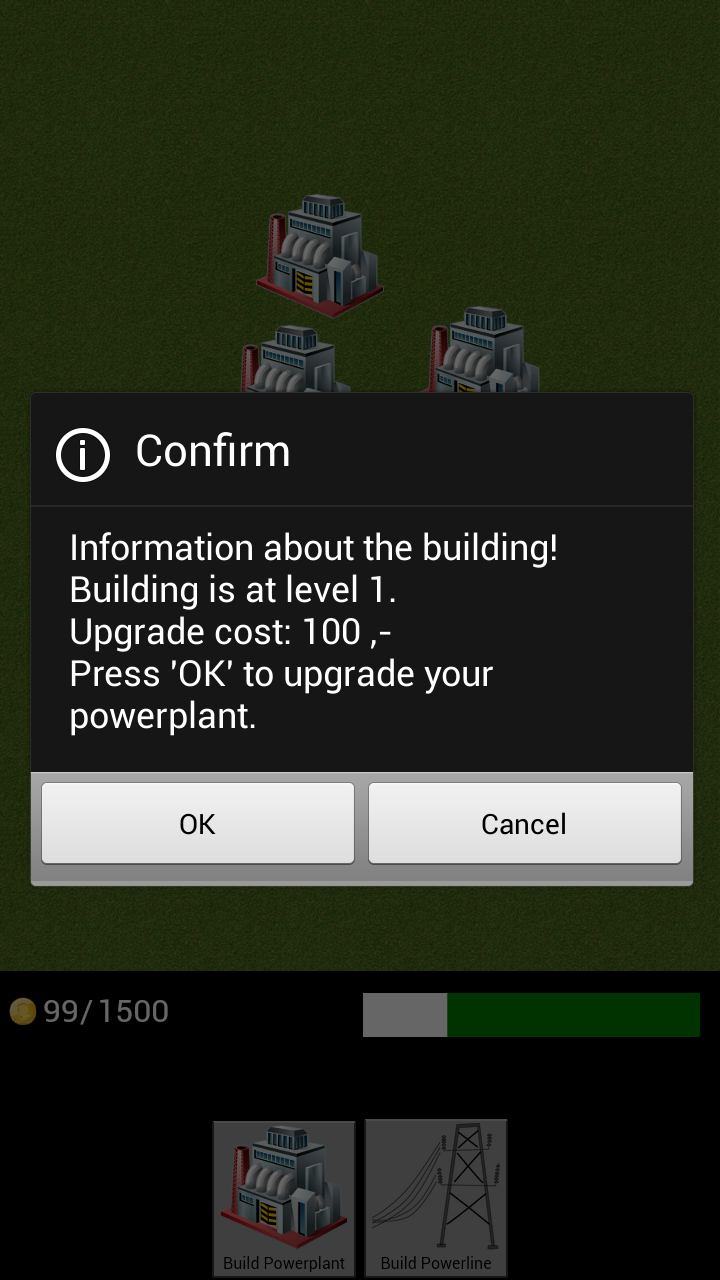
\includegraphics[scale=0.17]{pictures/sprint2-screen/sprint2-12}
	}
	\caption{Building Powerplants}
	\end{figure}

	\begin{figure}[H]
	\centering
	\subfigure{
		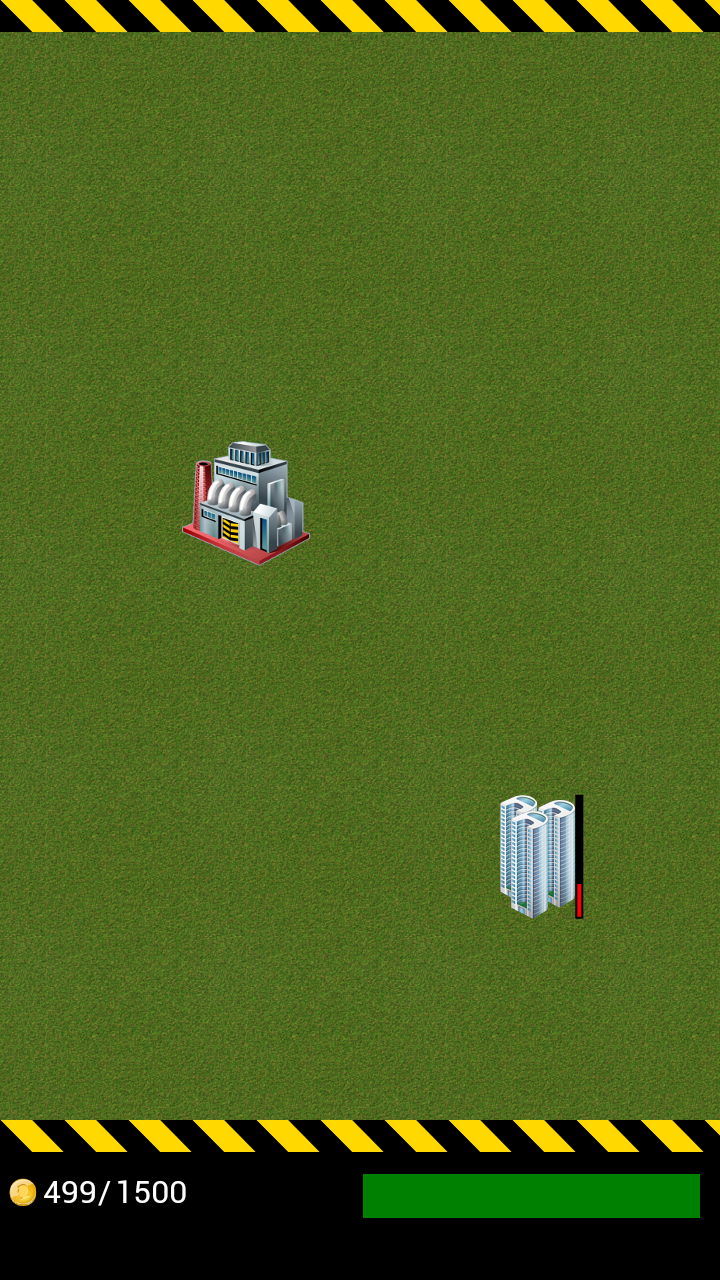
\includegraphics[scale=0.17]{pictures/sprint2-screen/sprint2-6}
	}
	\subfigure{
		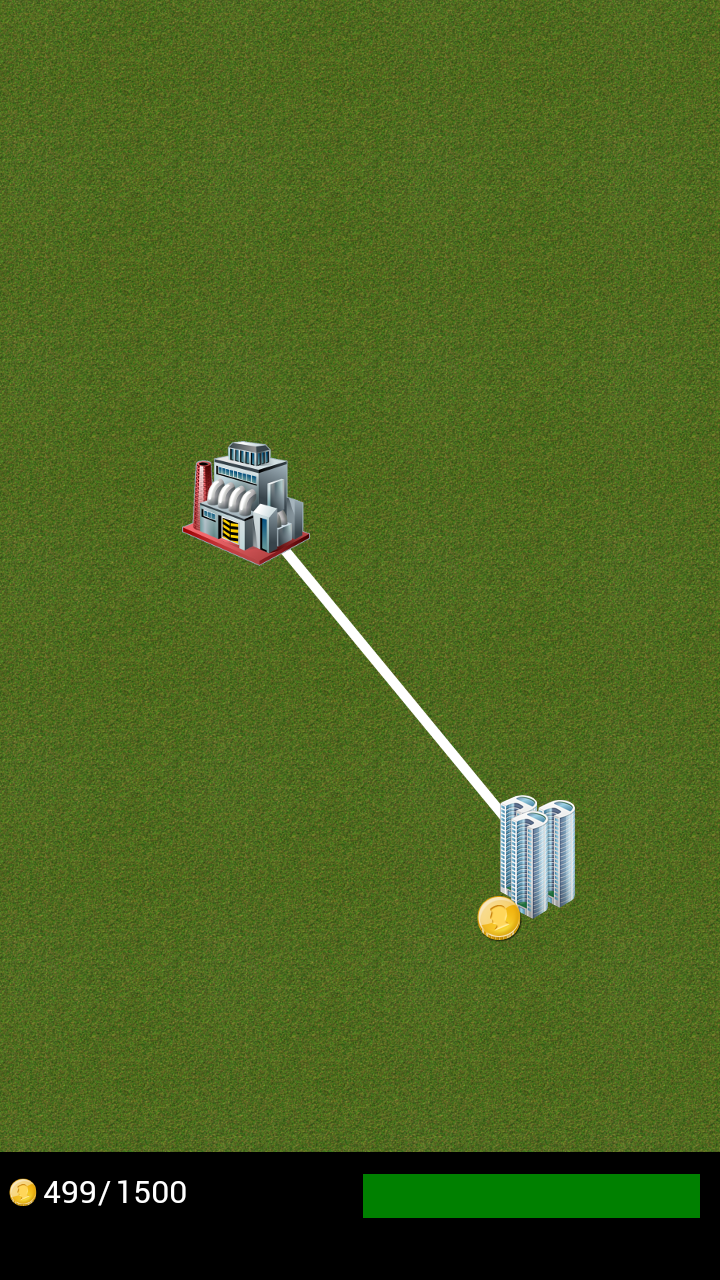
\includegraphics[scale=0.17]{pictures/sprint2-screen/sprint2-7}
	}
	\caption{Building Powerlines}
	\end{figure}

		\begin{figure}[H]
	\centering
	\subfigure{
		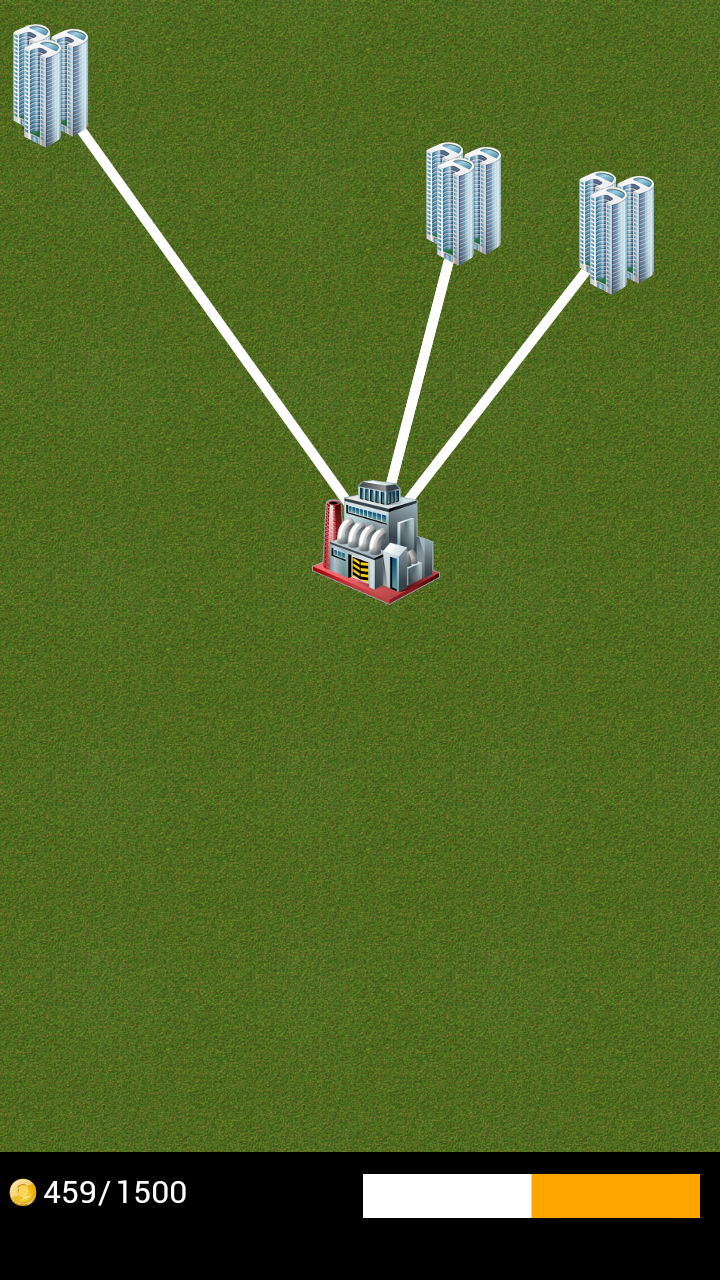
\includegraphics[scale=0.17]{pictures/sprint2-screen/sprint2-8}
	}
	\subfigure{
		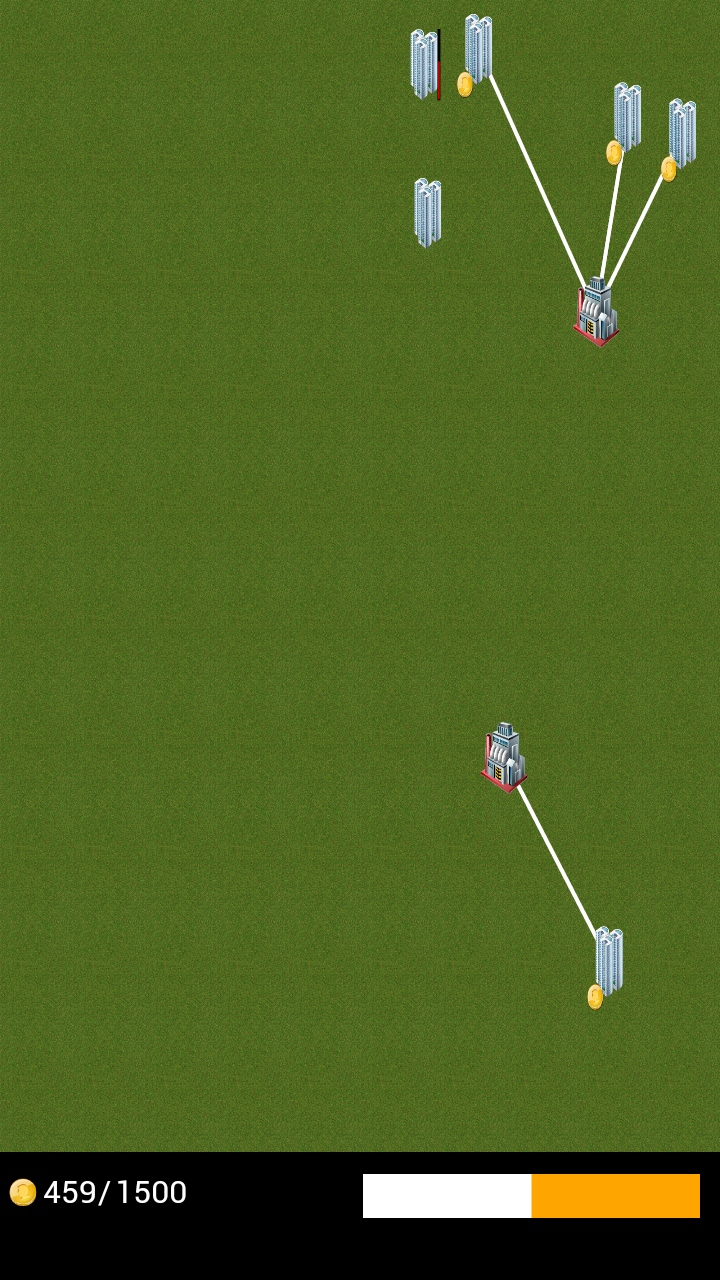
\includegraphics[scale=0.17]{pictures/sprint2-screen/sprint2-9}
	}
	\caption{Connecting multiple buildings}
	\end{figure}

	\begin{figure}[H]
	\centering
	\subfigure{
		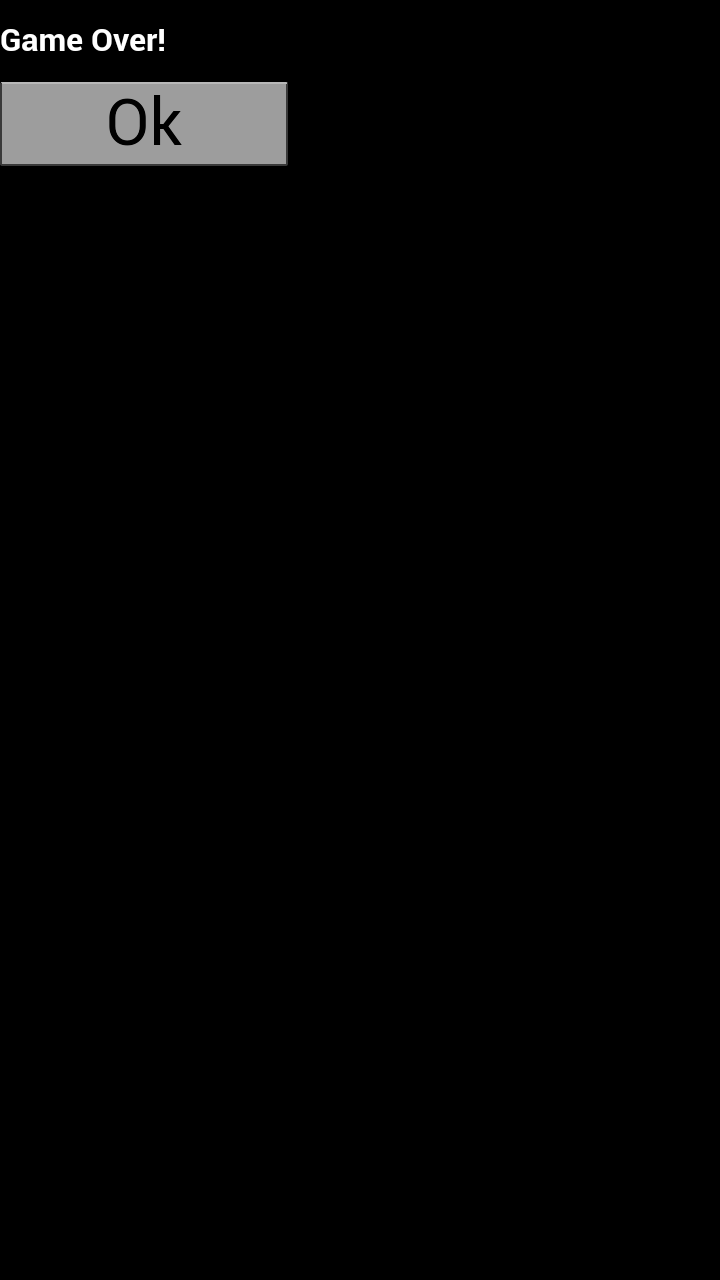
\includegraphics[scale=0.17]{pictures/sprint2-screen/sprint2-10}
	}
	\subfigure{
		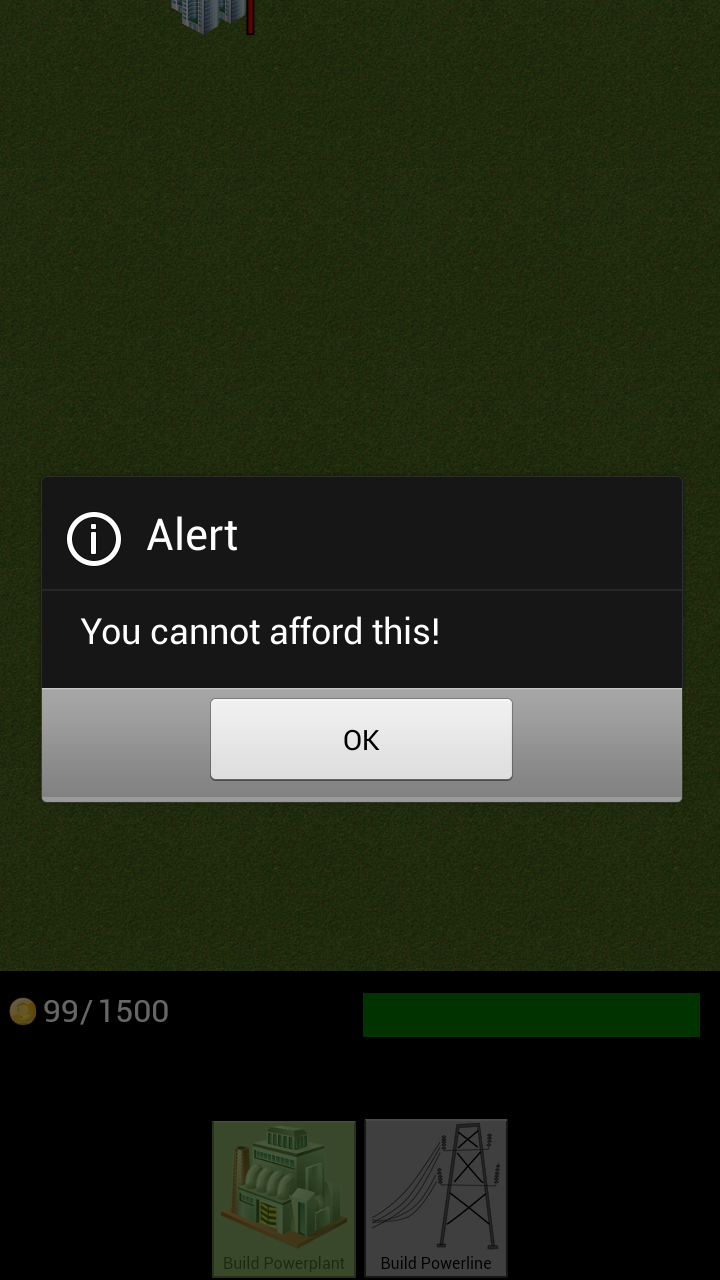
\includegraphics[scale=0.17]{pictures/sprint2-screen/sprint2-11}
	}
	\caption{Game over screen and ingame alerts}
	\end{figure}

\clearpage
\subsection{Testing}

	\subsubsection{Tests introduced in this sprint}

	The functional tests executed in this sprint are listed here. The test cases can be found in chapter 7.4.

	\definecolor{lightgray}{gray}{0.9}

	\begin{tabular}{| p{3cm} | p{7cm} | p{2cm} |}
		\hline
		\rowcolor{lightgray}
		{\bf Test Case} & {\bf Result} & {\bf Pass/Retest} \\ \hline
	  	
	  	FT-04 Main Menu & Works as expected. & Pass. \\ \hline

		FT-05 Build Power Plants & It is still possible to build on top of other buildings, otherwise it works as expected. Needs minor adjustment. &  Retest. \\ \hline

		FT-06 Build Power Lines & Building power lines is currently free, it is possible to connect a building to several power plants, and power lines may cross each other. Otherwise it works as expected. Needs adjustments.  & Retest. \\ \hline

		FT-07 Upgrade Power Plant & Upgrading a power plant does not yet affect the amount the power plant can supply. This will be implemented at a later stage. & Retest. \\ \hline

		FT-08 Information on Power Plants & Correct information is displayed when tapping a power plant & Pass.\\ \hline

		FT-09 Building Mode & Works as expected & Pass. \\ \hline

		FT-10 Tilting & Works as expected & Pass. \\ \hline

		FT-11 Collect Money & Works as expected & Pass. \\ \hline

		FT-12 No Power and Health Bar & Works as expected & Pass. \\ \hline

		FT-13 Game Over & Works as expected. & Pass. \\ \hline

	\end{tabular}

	\subsubsection{Redone tests}

	The following are the tests that has been executed again this sprint, because they did not pass last sprint:

	\begin{tabular}{| p{3cm} | p{7cm} | p{2cm} |}
		\hline
		\rowcolor{lightgray}
		{\bf Test Case} & {\bf Result} & {\bf Pass/Retest} \\ \hline

		FT-02 Appearance of buildings & Buildings appear at a more controlled rate and now has the ability to disappear. But they can appear on top of each other. Needs some minor adjustments. & Retest. \\ \hline

	\end{tabular}

\subsection{Changes to the requirements}
	In this sprint the group have made some changes. Since last sprint meeting, 
	the group hoped that the customer would change, add or remove requirements, 
	but this have not happened. During the implementation in this sprint, the 
	scrum team did come up with changes to the requirements. 
	Some requirements are moved, changed, split or removed.
	In the end of sprint 2 we had the version 3 of the requirement specification 
	and here are the changes:


	{\bf Changes on version 1 of the requirement specification:} \\
	\begin{tabular}{| p{1.5cm} | p{12cm} |}
		\hline
		\rowcolor{lightgray}
		{\bf FR} & {\bf Change} \\ \hline
		FR3.3 & {\bf \color{green} [NEW]} There should be several types of buildings on the map, 
		with different power requirements  \\ \hline
		FR3.4 & {\bf \color{green} [NEW]} Different types of building should reward different amounts of 
		money \\ \hline
		FR3.6 & {\bf \color{orange} [CHANGED]}changed priority from high to critical \\ \hline
		FR4.4 & {\bf \color{red} [REMOVED]} As the user reaches higher levels there should be an 
		increase in faulty power cables \\ \hline
		FR5.2 & {\bf \color{red} [REMOVED]} There should be buildings on the map for the user to 
		supply with power; new buildings should appear over time. \\ \hline
		FR5.4 & {\bf \color{red} [REMOVED]} The player should be able to suspend specific buildings' 
		power supply in order to server others \\ \hline
		FR5.5 & {\bf \color{orange} [MOVED TO GUI]} A power preservation tip should appear when the 
		user reaches a new level. \\ \hline
	\end{tabular}

	{\bf Changes on version 2 of the requirement specification:} \\
	\begin{tabular}{| p{1.5cm} | p{12cm} |}
		\hline
		\rowcolor{lightgray}
		{\bf FR} & {\bf Change} \\ \hline
		FR1.9 & {\bf \color{green} [NEW]} There should be played a sound effect when 
		the player collects money \\ \hline
		FR1.10 & {\bf \color{green} [NEW]} There should be played a sound effect when 
		the player upgrades the power plant \\ \hline
		FR1.11 & {\bf \color{green} [NEW]} There should be played a sound effect when 
		the player builds a power cable \\ \hline
		FR1.12 & {\bf \color{green} [NEW]} The user should not get the opportunity to 
		tilt the screen by tilting the phone. \\ \hline
		FR2.4 & {\bf \color{orange} [MOVED TO INCOMING/OUTGOING MONEY]} The user should 
		be able to connect the buildings to the power plants by building a power cable. 
		Building cables costs money. \\ \hline
		FR3.6 & {\bf \color{green} [NEW]} When an existing building is not supplied 
		with power within a certain amount of time, the house should disappear and the player's 
		health score should decrease \\ \hline
		FR3.6 & {\bf \color{orange} [MOVED TO GUI]} The user should be able to see 
		that a building has gone without power for some time, and is affecting the 
		player's health score if the building is not connected to a power plant before it 
		disappears. \\ \hline
		FR4.3 & {\bf \color{orange} [MOVED TO OBSTACLES]} When an existing building 
		is not supplied with power within a certain amount of time, the house should 
		disappear and the player's health score should decrease \\ \hline
		FR5.4 & {\bf \color{green} [NEW]} The user should be able to upgrade the power plant. 
		This cost money. \\ \hline
		FR6.7 & {\bf \color{green} [NEW]} The user should be able to see the main 
		menu when he or she starts the game. \\ \hline
		FR6.8 & {\bf \color{green} [NEW]} When the player wants to place a power plant 
		or a power cable in building mode, the player should be prompted if they want to 
		go through with it, or cancel. \\ \hline
		FR6.9 & {\bf \color{green} [NEW]} The user should be able to see that he or she 
		is in building mode when selecting a building to build in the hub menu. \\ \hline
	\end{tabular}

\subsection{Group dynamics}
	In sprint 1 the group had some problems with the group dynamics. 
	During this sprint we managed to work together as a group and the group dynamics
	is now very good. The changes that helped the group to work better as a group
	was the allocation of roles in the last sprint. 

\subsection{Customer feedback}
	In this sprint the group got a feedback from the customer in the end of the sprint.
	The customer think that we are working structured and the flow of information is good.
	They are very pleased with the cooperation this far in the project.

	After the sprint meeting, the customer tested the game on a phone. The feedback on the game
	was that they had some problems with building the power lines as well as knowing how to play.
	The group will try to solve the problems until the next meeting.

	The customer is also very pleased with the requirement specification and the priorities
	that we have made. So far, the group has implemented the most of the critical and high
	priorities and the requirements left in the backlog is mainly medium/low. 

\subsection{Sprint retrospective}
	\subsubsection*{Start doing: } 
		\begin{itemize}
			\item use branches for new features to be implemented and not implement new 
			features in the master branch.
		\end{itemize}
	\subsubsection*{Stop doing: }

	\subsubsection*{Continue doing: }
		\begin{itemize}
			\item Keep up the good team work
		\end{itemize}


\clearpage
\section{Sprint 3}

\subsection{Sprint planning}
	In sprint 3 the group planned to implement the final requirements with high priority, as well as most of the requirements with medium priority. This is the second to last sprint, and it is important that in the last sprint the  only remaining requirements are medium to low requirements, so that time can also be spent fixing bugs and make the game work properly on iOS. The goal for this sprint will be to get a fully playable game, with only minor requirements missing.

	A usability test will be carried out in the last week of the sprint to discover potential bugs or errors we have yet to discover, as well as ideas for improvements that may be implemented in the next sprint.

	Concerning the report, we plan to finish the chapters up until this sprint.

\subsection{Duration and Workload}
	
	{\bf Duration:} 14.10 - 27.10 (2 weeks)\\
	{\bf Workload:} This is the list with hours spent (the whole group) on the project in this sprint.
	\begin{itemize}
		\item {\bf Planning:} 15.5 hours
		\item {\bf Development:} 44 hours
		\item {\bf Design:} 0 hours
		\item {\bf Documentation (report):} 59.5 hours
		\item {\bf Testing:} 20.5 hours 
	\end{itemize}
	{\bf Total workload: } 139.5 hours \\
	
	The group's goal was to work at least 20 hours per person every week in this sprint. 
	The group did manage the a workload with an average of 17.4 hours/week (139.5 hours/4 persons/2 weeks = 20.6 hours). The reason for the low numbers is because one of the group members did not
	participate as much as he should. The 3 other group members did work over 20 hours. 


\clearpage
\subsection{Sprint Backlog}
	\begin{table}[H]
	\begin{tabular}{| p{1cm} | p{7cm} | p{2cm} | p{2cm} |}
		\hline
		\rowcolor{gray}
		ID & Description & Estimate & Actual effort \\ \hline

		FR2.5 & The amount of power available to the user should be limited; 
		the power supply of a power plant should be upgradeable. 
		& 3 hours  & 1 hour \\ \hline

		FR2.6 & The user should be able to remove power lines from the 
		& 10 hours & 5 hours \\ \hline

		FR3.1 & Arbitrary power lines may be damaged throughout the game 
		& 5 hours & 10 hours \\ \hline

		FR3.2 & The user should be able to fix unstable power lines before it is 
		broken; this should cost some amount of money. 
		& 6 hours & 5 hours \\ \hline

		FR3.3 & There should be several types of buildings on the map, with different 
		power requirements 
		& 2 hours & 2 hours \\ \hline

		FR3.4 & Different types of building should reward different amounts of 
		money 
		& 3 hours & 1 hour \\ \hline

		FR4.1 & The user should be able to continue to the next level when the goal is 
		reached 
		& 3 hours & 2 hours \\ \hline

		FR4.3 & As the user reaches higher levels new buildings appear more 
		rapidly 
		& 3 hours & 2 hours \\ \hline

		FR4.4 & As the user reaches higher levels unstable power lines will appear 
		more rapidly 
		& 2 hours & 2 hours \\ \hline

		FR4.5 & As the user reaches higher levels the map size may increase 
		& 2 hours & 2 hours \\ \hline

		FR4.6 & The user should be able to win the game by reaching the goal in 
		the current level. The goal is level specific. 
		& 3 hours & 2 hours \\ \hline

		FR5.2 & When connecting buildings through power lines, there should be a 
		cost which is proportional to the length of the power line. 
		& 2 hours & 3 hours \\ \hline

		FR6.11 & The user should be able to see which houses is selected when 
		building power lines 
		& 2 hours & 2 hours \\ \hline

		FR6.12 & The power lines should change color if it is connected to a power 
		station. 
		& 2 hours & 2 hours \\ \hline

		FR6.13 & The user should be able to see how much power the power plant have 
		left. This bar should decrease if a building is connected to the power plant 
		and should be increase if a building is removed. The colors should be yellow 
		with white background. 
		& 3 hours & 3 hours \\ \hline

	\end{tabular}
	\caption{Sprint backlog sprint 3}
	\end{table}

\subsection{Implementation}
	
	\subsubsection{Power Lines}
		\begin{itemize}
			\item {\bf Build Power Lines: } the user is now able to build powerlines
			between buildings. There is no restrictions of what buildings you can connect, 
			but there need to be a powerplant in the connected buildings in order to serve the houses 
			with power.
			\item {\bf Remove Power Lines: } there is implemented a remove powerline. The 
			algorithm used is described under "algorithms" in this section. 
			\item {\bf Damaged Power Lines: } it was implemented functionality to set a 
			powerline to be in "damaged" mode. 
			\item {\bf More damaged power lines in new levels: } when the user reaches a higher level
			there is now appearing more damaged power lines that needs to be fixed. 
			\item {\bf Color of power line: } A powerline is black if there is no power served between
			the buildings. The reason for a line to be black is either is there is no poweplant
			connected og if the powerplant cannot serve the houses. If the line is yellow, it 
			signalize that there is sent power to the house. 
			\item {\bf Selected houses when building powerlines: } when building a powerline, 
			the user tap on the building he or she wants to connect the line between. When tapping on the
			first house, it is 
		\end{itemize}

	\subsubsection{Other Implementations}
		\begin{itemize}
			\item {\bf Collect Money: } when a building is connected to a powerplant, it starts
			"producing" money. The money icon is added to the building and the user is now
			able to click on the building in order to collect the money. The players money
			should increase and be more close to the goal. 
			\item {\bf Enter next level: } a user should be able to complete a level by getting
			as much money as the goal for the specific level. For example if the goal is 1500, the
			player reach the next level by getting his/her sum of money equal or greater than 1500.
			\item {\bf Powerplant with Limited Power: } a powerplant do not have infinite amount of
			power. The powerplant can be upgraded to serve more power. 
			\item {\bf Number of Power Plants: } this is not implemented yet, but it should be added
			to the next sprint. 
			\item {\bf Different Buildings: } when the time loop have started, there is appearing
			different type of buildings. Each house require a different amount of money and is
			also "producing" a different amount of money when the building is served with power
			form a powerplant. 
			\item {\bf Appearance of buildings in new levels: } buildings appear more rapidly 
			when the level increase. 
		\end{itemize}
	
	\begin{figure}[H]
		\centering
		\subfigure{
			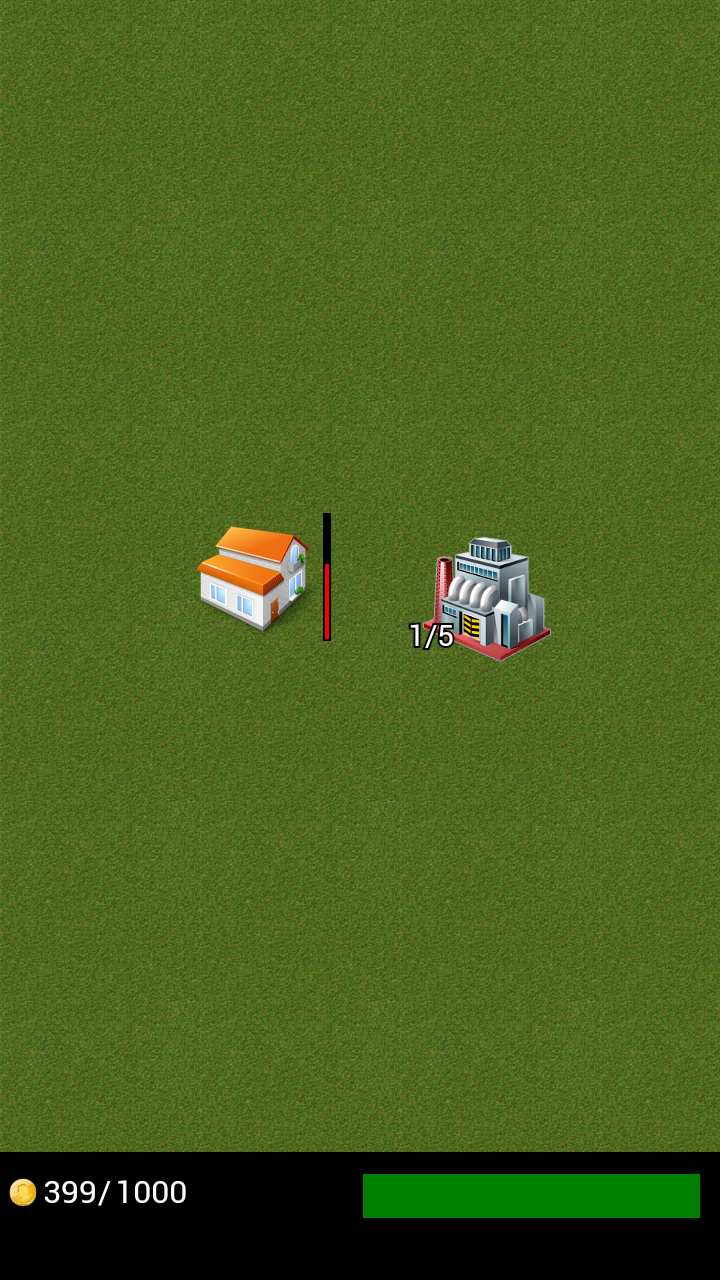
\includegraphics[scale=0.18]{pictures/sprint3-screen/buildPowerline_1.png}
		}
		\subfigure{
			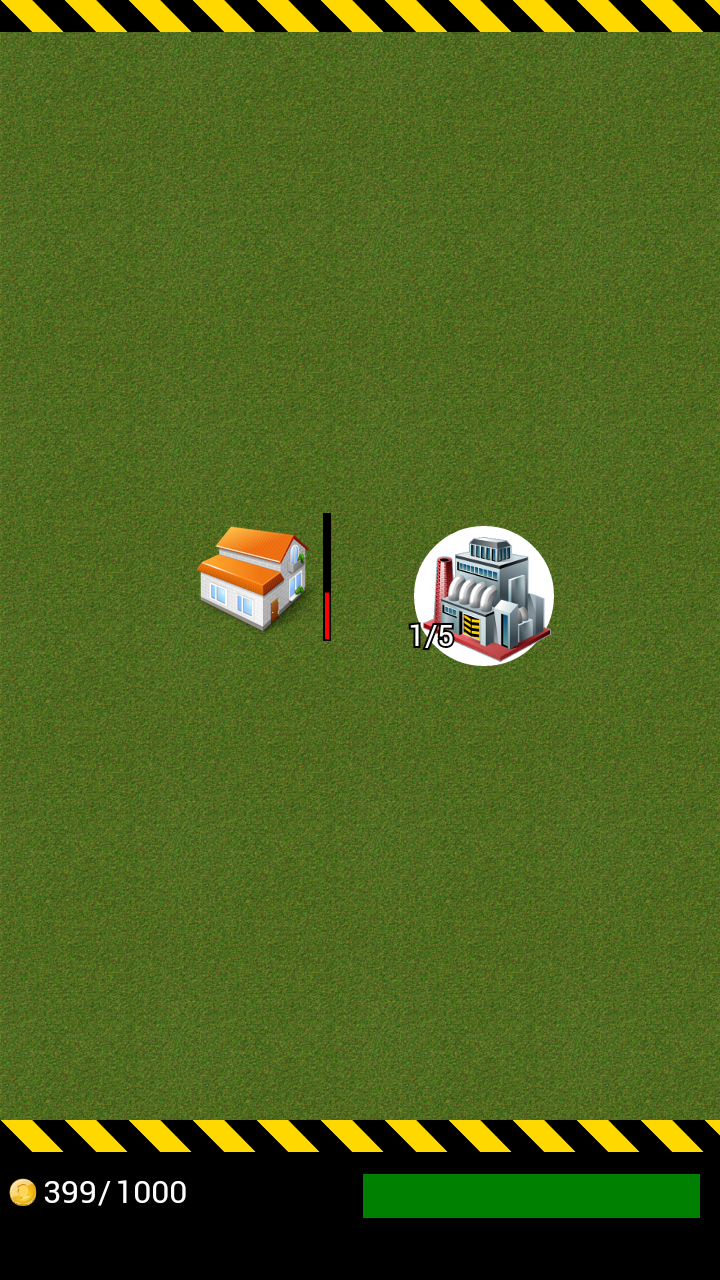
\includegraphics[scale=0.18]{pictures/sprint3-screen/buildPowerline_2.png}
		}
		\caption{User connecting buildings}
	\end{figure}
	\begin{figure}[H]
	\centering	
		\subfigure{
			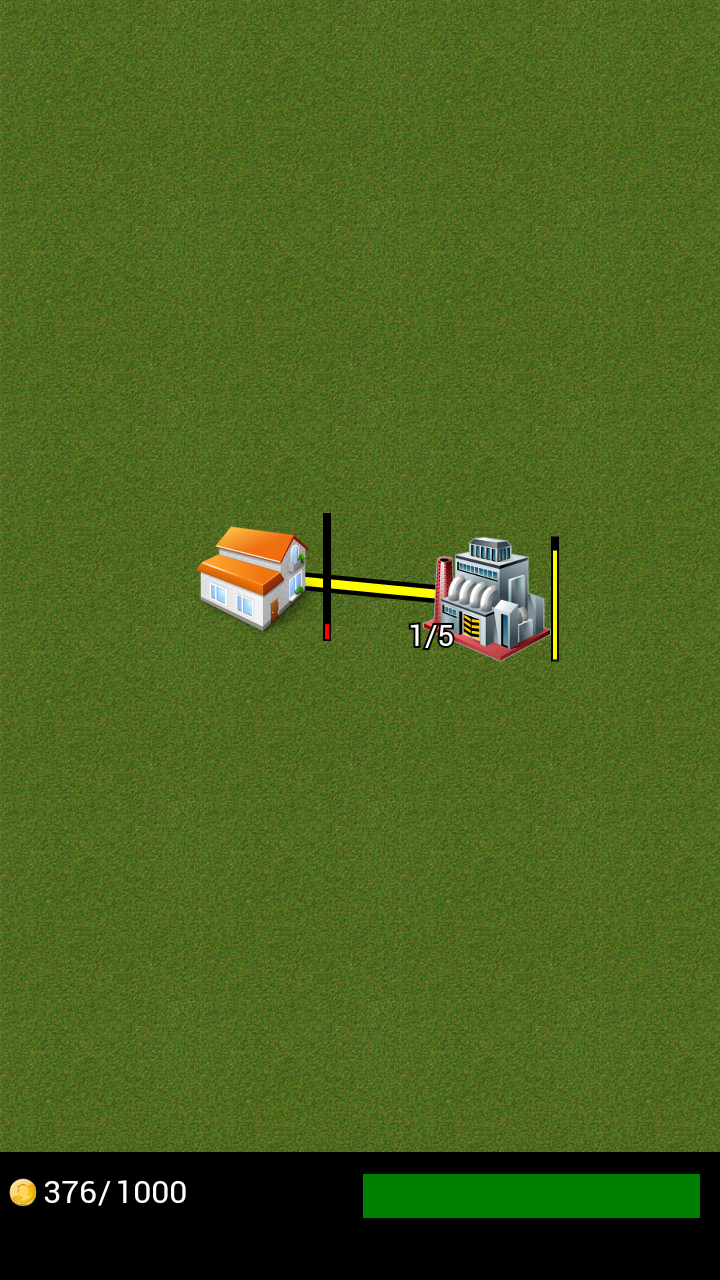
\includegraphics[scale=0.18]{pictures/sprint3-screen/buildPowerline_4.png}
		}
		\subfigure{
			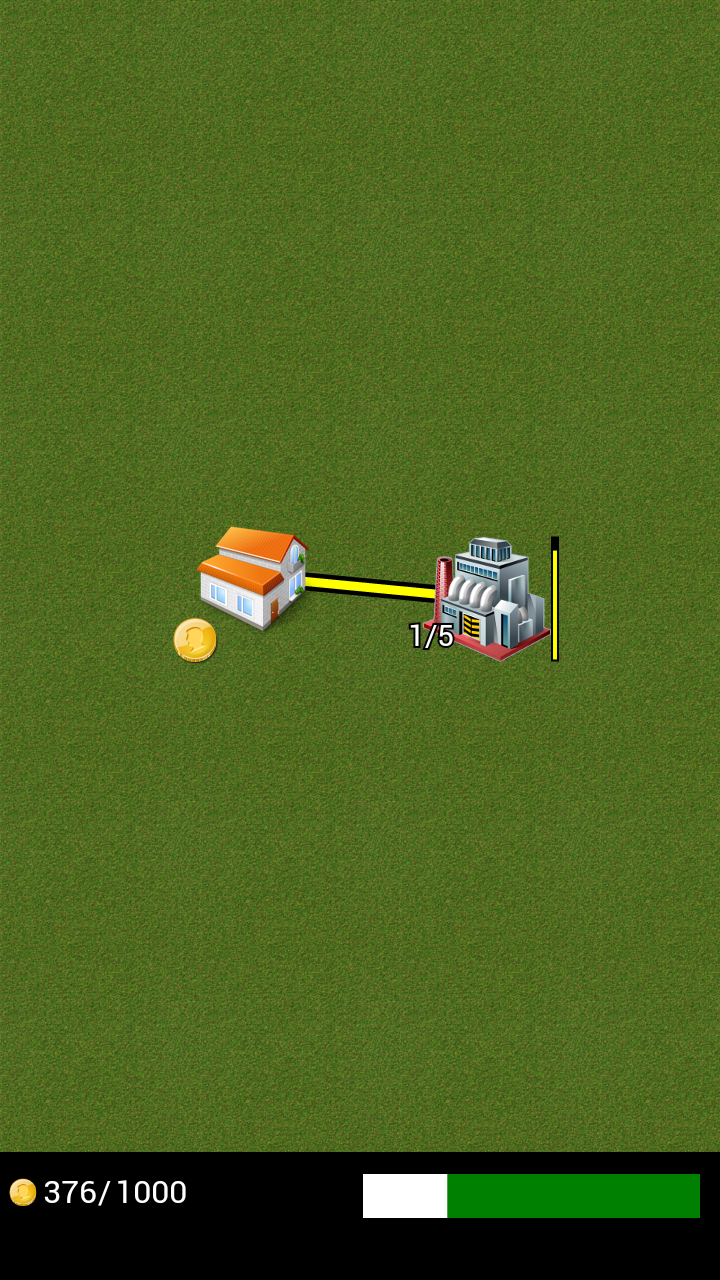
\includegraphics[scale=0.18]{pictures/sprint3-screen/buildPowerline_5.png}
		}
		\caption{Power is served and money can be collected}
	\end{figure}

	\begin{figure}[H]
		\centering
		\subfigure{
			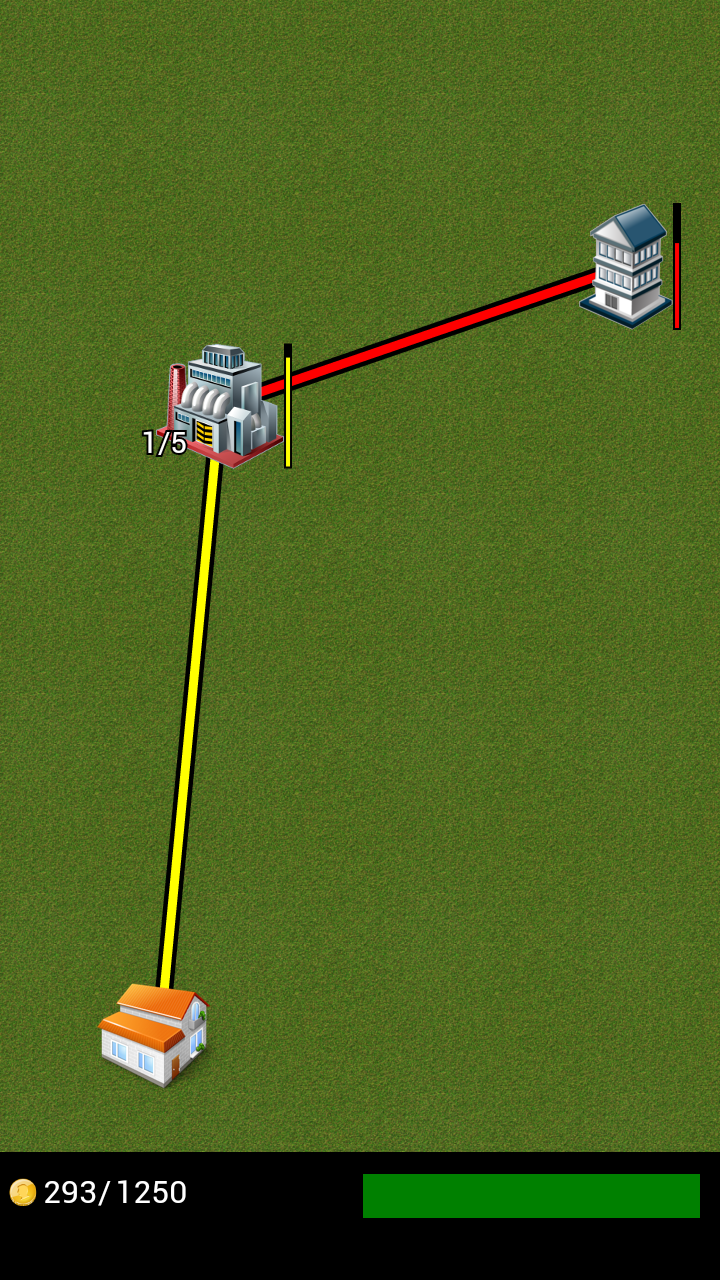
\includegraphics[scale=0.18]{pictures/sprint3-screen/damaged.png}
		}
		\subfigure{
			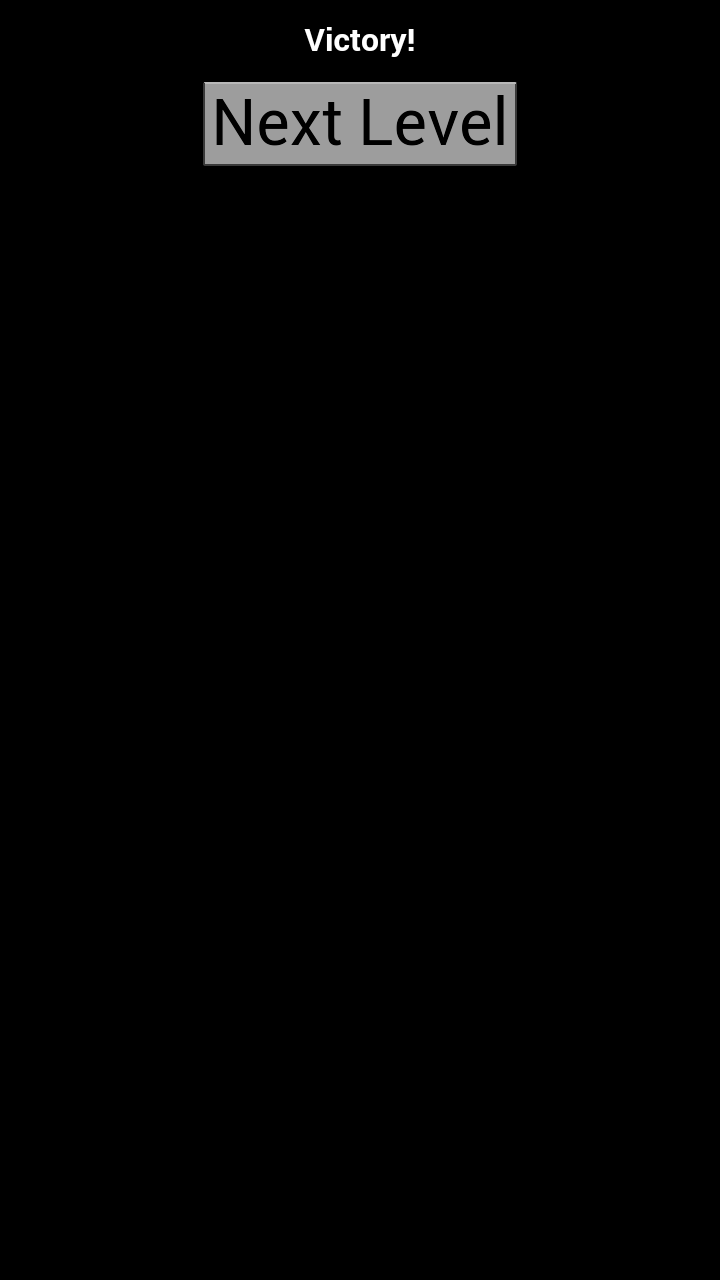
\includegraphics[scale=0.18]{pictures/sprint3-screen/nextLevel.png}
		}
		\caption{Damaged red powerline and next level screen}
	\end{figure}

	\begin{figure}[H]
		\centering
		\subfigure{
			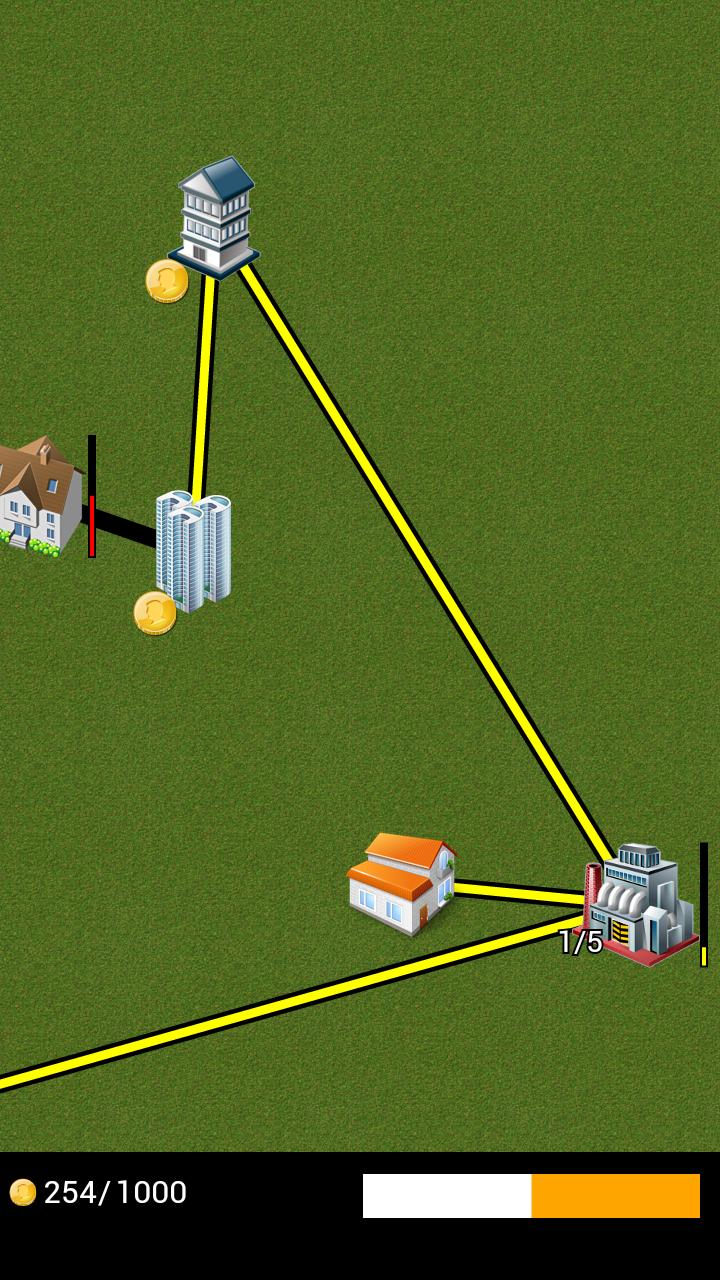
\includegraphics[scale=0.18]{pictures/sprint3-screen/notServe.png}
		}
		\subfigure{
			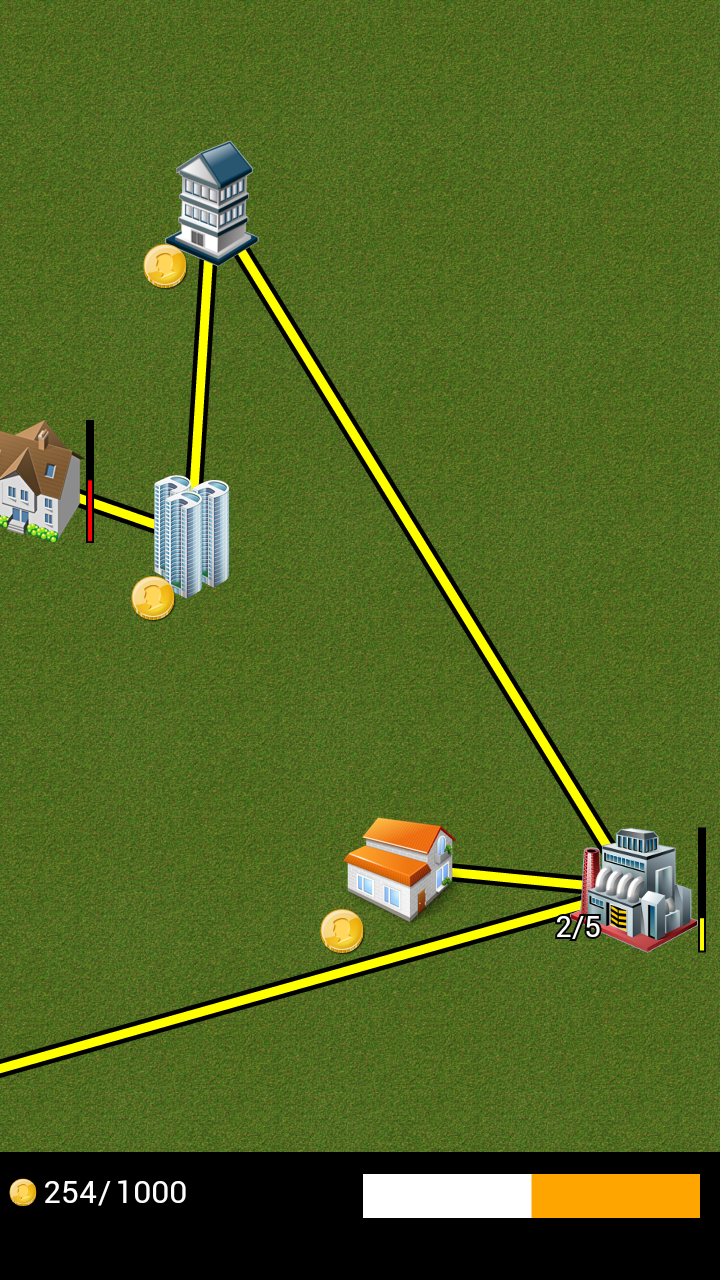
\includegraphics[scale=0.18]{pictures/sprint3-screen/serve.png}
		}
		\caption{Upgrade Powerplants to deliver more power}
	\end{figure}

	\subsection*{Algorithms}
		\begin{itemize}
			\item{\bf Breadth First Search}
			Breadth First Search is a standard algorithm taught in both Discrete Mathematics and 
			Algorithm courses. Breadth First Search (from now on refered to as BFS) traverses a graph 
			by exploring one level of the graph at a time. BFS is used to distribute power from the 
			power plants to the buildings on the map. The graph is defined by having all buildings 
			and power plants be vertices and the power lines are edges. The algorithm runs once for 
			each power plant on the map every time there is a change to the graph.

			\item {\bf Point to Line Segment Distance}
			The Point to Line Segment Distance algorithm works by projecting the point \emph{p} onto the line 
			defined as going through the point \emph{v} and the point \emph{w}. Then the algorithm 
			examines the following three different locations for the projection on the line: 
			\begin{enumerate}
				\item Before \emph{v}.
				\item After \emph{w}.
				\item Between \emph{v} and \emph{w}.
			\end{enumerate}
			If the projection lies before \emph{v} on the line, then the distance from \emph{p} to 
			the line segment from \emph{v} to \emph{w} is simply the distance from \emph{p} to 
			\emph{v}. If the projection lies after \emph{w} on the line, then the distance from 
			\emph{p} to the line segment is the distance from \emph{p} to \emph{w}. In the last case 
			where the projection lies between \emph{v} and \emph{w}, the answer is the distance from 
			\emph{p} to the location of the projection. There is also the special case where the 
			length of the line segment from \emph{v} to \emph{w} is 0. In that case the distance 
			from \emph{p} to the line segment is just the distance from \emph{p} to either \emph{v} 
			or \emph{w}.\cite{pldTheory}\cite{pldCode}

			\begin{figure}[H]
			\centering
			\subfigure{
				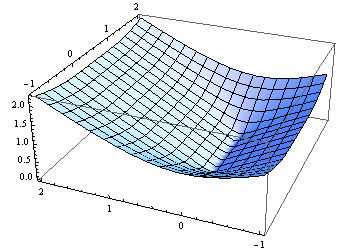
\includegraphics[scale=0.75]{pictures/PtLSplot}
			}
			\caption{Plot of Point to Line Segment Distance}
			\end{figure}
		\end{itemize}

\subsection{Functional Testing}

	The following test cases were executed at the end of this sprint:

	\definecolor{lightgray}{gray}{0.9}

	\begin{table}
	\begin{tabular}{| p{3cm} | p{6.5cm} | p{2.5cm} |}
		\hline
		\rowcolor{lightgray}
		{\bf Test Case} & {\bf Result} & {\bf Pass/Retest} \\ \hline

	  	FT-14 Complete Level & Works as expected. & Pass. \\ \hline
	  	
	  	FT-15 Limited Power & Works as expected. & Pass. \\ \hline
	  	
	  	FT-16 Remove Power Line & Works as expected. & Pass. \\ \hline
	  		  	
	  	FT-17 Different Buildings & Works as expected. & Pass. \\ \hline

	  	FT-18 Damaged Power Lines & Power lines are damaged throughout the game, but are not possible 
	  	to fix at the moment. & Retest. \\ \hline
	  	
	  	FT-19 Enter next level & Works as expected. & Pass. \\ \hline

	  	FT-20 Appearance of buildings in new levels & Works as expected. & Pass. \\ \hline

	  	FT-21 More unstable power lines in new levels & Works as expected. & Pass \\ \hline

	  	FT-22 Selected houses & Works as expected. & Pass. \\ \hline

	  	FT-23 Color of power lines & Works as expected. & Pass. \\ \hline
	  	FT-24 Map size in new levels & Works as expected. & Pass \\ \hline

	\end{tabular}
	\caption{Functional tests from sprint 3}
	\end{table}

	The following test cases did not pass previous tests and were retested this sprint:

	\begin{table}
	\begin{tabular}{| p{3cm} | p{6.5cm} | p{2.5cm} |}
		\hline
		\rowcolor{lightgray}
		{\bf Test Case} & {\bf Result} & {\bf Pass/Retest} \\ \hline

		FT-02 Appearance of buildings & Building can still appear on top of each other & Retest. \\ \hline

	  	FT-05 Build Power Plants & The power plants are still possible to place on top of other buildings & Retest. \\ \hline

	  	FT-06 Build Power Lines & The power lines now cost money. It is still possible to build power lines that cross each other and it is still possible to connect several power lines to one building. & Retest. \\ \hline

	  	FT-07 Upgrade Power Plant & The amount of power the power plant can supply is now increased by an upgrade. & Pass. \\ \hline
	\end{tabular}
	\caption{Redone tests in sprint 3}
	\end{table}

\subsection{Usability Test}

	This sections presents the results from the usability test that was carried out in this sprint. The usability test proved to be very helpful in terms of increasing the user friendliness of the user interfaces and making the game more enjoyable to play. More information on how the usability test was planned and carried out can be found in chapter 7.5 Usability Test.

	\subsubsection*{How far the game was from completion}

	The most apparent missing feature in the game at the time of testing was the possibility 
	to fix damaged power lines. At this point a damaged power line had to be removed and then 
	rebuilt. There are still no boundaries for where buildings can appear within the map, or 
	where power plants can be placed. Another aspect that affected the testing was that the balance 
	between the game parameters, for a given level, were not optimal as this was something that 
	would be difficult and time consuming to get just right. The parameters are the rate at which 
	buildings appear, the rate at which the health bar decreases when a building disappears, 
	how long it should take for a house without electricity to disappear, how much power a power 
	plant should be able to serve and how much effect an upgrade should have, and lastly how much 
	building should cost and how much money one should earn from the households. One game parameter 
	that affected the testing was the fact that the health bar decreased extremely slowly, a house 
	disappearing had almost no effect on the health bar. The objective was to not get a game over too fast, 
	and to not stress the testers while playing so that they had time to give us their thought 
	while playing. When looking back the health bar could have decreased faster and still not 
	make the game end too fast. Other features that were not implemented but did not noteworthy 
	affect the testing was high score, pausing the game and sounds.

	\subsubsection*{Feedback from the usability test}%\mbox{}\\

		\textbf{Zooming}
			Some testers found double tapping to zoom non-intuitive, and some wished it had 
			been possible to zoom by placing the thumb and pointer finger at opposing points 
			of the screen and moving the fingers away from each other.

			Several people wished it was possible to build also in zoomed-out mode.

		\textbf{The Hud}
			Those who had not read the game instructions in advance had trouble finding out that 
			the hud was possible to move up.

			Some people found the goal to be unclear and did not notice the "players money" vs. "goal" at the bottom of the screen.

			Several players did not understand what the health bar was, but when they were told what it was they understood it. A possible reason to why they did not understand that it was a health bar is explained in the section "How far the game was from completion".

		\textbf{The Coins}
			Several players ignored the coins because they did not know they had a function.

			All the players struggled with collecting money from the households. The reason for this was that they tapped the coin instead of the building and this lead to the money not being collected.

		\textbf{Power Lines}
			Many people had trouble understanding that the red power line indicated that the power line was damaged, and some thought it meant that there were not enough power.

			One person had trouble understanding that power line could be connected between buildings and connected them all directly to the power plant.

			At some points the players found it hard to tap the power line if it was to small.

		\textbf{Power Plants}
			It was not obvious to the players what the number on the power plant meant, i.e. the number indicating the number of upgrades done and the number of upgrades still available. Most of the players also did not understand that it was possible to upgrade the power plant, which might have led to the confusion about the numbers.

		\textbf{Buildings}
			Not everyone understood what the bar belonging to the house was, and some assumed that when the house disappeared they were punished in some way, but was unsure how. This may be caused by the fact that a disappearing house had little effect on the health bar.

			One player found it hard to play when buildings appeared very closed or almost on top of each other.

		\textbf{Other}
			At the very beginning of a new game, before the first house appeared nothing seemed 
			to be happening and this confused many of the testers.

			One player missed a sign telling him which level he was at.

			Some players wanted an in-game introduction to the different elements of the game and how it was played.

	\subsubsection*{Results of the Feedback}

	The following are suggestions to changes and improvements that should be made, as a result of the feedback from the usability test.

	Each level should start with an alert message that tells the player how much money he or she needs to earn in order to reach the next level. This will make the player more aware of what the goal is and that it is changing and will hopefully make the start of a new game less confusing.

	The zoomed out mode was intended for just giving an overview of the state of the game, making the game a little harder considering that the player did not know of all buildings needing power at all time, but if the possibility to build in zoomed-out mode will make the game more enjoyable, then this will be done.

	There should be an indication that the hud can be lifted into view, such as some form of handle, but considering the feedback from the customer, the building icons should always be visible in game mode to make building more effectively, thus solving both issues. One user liked that the hud was not visible because this made more room for the map, but we will strive to make the icons not clogging the screen.

	When collecting money, it is obviously more intuitive to tap the coin as opposed to the building. The coin will be moved closer to the building, so that when tapping the coin, the building will also be tapped, and as a result the money will be collected.

	It should be made clearer to the player that a power line is damaged. This can be done by making a cut to it. It should still be red to attract the attention of the player.

	In order to make it more visible to the player that the power plants can be upgraded, an arrow of some sort should be placed over the building.

	Which level the player is at should be visible when playing.

	\subsubsection*{Result of usability survey}

	The table below shows the average score for a given question or statements along with an explanation to the scale for the specific question. The question form as presented to the users can be found in Appendix F.

	\begin{table}[H]
	\begin{tabular}{| l | p{5cm} | p{1cm} | p{5cm} |}
  		\hline
		\rowcolor{gray}
		{\bf Nr.} & {\bf Question} & {\bf Avg Score} & {\bf Scale} \\ \hline
		
		1. & I think that I would like to play this game frequently. & 2.75 & 1 = not frequently, 5 = frequently\\ \hline

		2. & I found the game unnecessarily complex. & 2 & 1 = not complex, 5 = complex \\ \hline

		3. & I thought the game was easy to understand. & 3.5 & 1 = hard to understand, 5 = easy to understand \\ \hline

		4. & I thought there was too much inconsistency in this game. & 2 & 1 = not inconsistent, 5 = inconsistent \\ \hline

		5. & I would imagine that most people would learn to play this game very quickly. & 4 & 1 = not easy to learn, 5 = easy to learn \\ \hline

		6. & I found the game very cumbersome to play. & 2.5 & 1 = not cumbersome, 5 = cumbersome \\ \hline

		7. & I felt very confident playing the game. & 3.25 & 1 = not confident, 5 = confident \\ \hline

		8. & I needed to learn a lot of things before I could start playing the game. & 2.75 & 1 = needed to learn a lot, 5 = did not need to learn a lot \\ \hline

		9. & Game Instructions/Rules. & 2 & Simple - Average - Complex \\ \hline

		10. & Luck vs. Skill. & 4 & Pure luck - Average - All skill \\ \hline

		11. & How much did you like the graphics? & 4 & Did not like - OK - Loved \\ \hline

		12. & Game Idea (Concept). & 3.75 & Boring - OK - Terrific \\ \hline

		13. & How much did you like this game? & 3.5 & Hated it - OK - Loved it \\ \hline

		14. & How often would you play this game? & 2.5 & Never again - Now and then - A lot \\ \hline

		15. & Options for what you can do in the game. & 2.5 & Not enough - Just right - Too many \\ \hline

		16. & Game map size. & 3 & Too small - Just right - Too big \\ \hline

		17. & Game elements (size). & 3 & Too small - Just right - Too big \\ \hline

		18. & Text size. & 3 & Too small - Just right - Too big \\ \hline
	\end{tabular}
	\caption{Results of usability survey}
	\end{table}

	It needs to be stated that only 5 users answered this survey, and in order to smooth over the 
	variability in the individual differences in the users, we should have had at least 20 of them. 
	\cite{quantitativeTest} That does not mean that the numbers gathered holds no value and we will take a look at some of them. 

	All in all the scores are quite centered around the middle score of 3. If we look at how much or frequently the users thought they would play it the score was a little below the average "Now and then". If we look at how easy the game was to understand, they thought the game was above average easy to understand, and they thought people would learn how to play the game quite quickly. The users found the game a little below average cumbersome, and quite easy to play. They were quite positive to the game idea and their thought on how much the liked the game was a little above "OK".

	Many of the scores could have been better, this was however only an unfinished prototype of the game, still with bugs, and several improvements was made to the game after the feedback from the testers. These changes could hopefully make the game easier to understand and less cumbersome to play and subsequently more fun.

\subsection{Changes to the Requirements}

	The first change to the requirements during sprint 3 was the change of priority in requirement FR 1.2. The priority was changed from high to medium, because it is not an essential feature to have in order to have a working game, but can still be an improvement in the user experience.

	The requirements FR 6.5 and FR 3.5 were duplicates and were removed. The visual notification will not be implemented. The group defined a sound as a notification and added requirement FR 1.13.

	Other requirements were also added as the group discovered that they were either missing or would be an improvement to the design.
	
	\begin{table}[H]
	\begin{tabular}{| p{1.5cm} | p{12cm} |}
		\hline
		\rowcolor{lightgray}
		{\bf FR} & {\bf Change} \\ \hline
		FR 1.2 & {\bf \color{orange}[CHANGED PRIORITY FROM HIGH TO MEDIUM]} The user should be able 
		to exit the game at any time, and the game state should be saved and loaded when the user 
		returns to the game \\ \hline
		FR1.13 & {\bf \color{green}[NEW]} The user should get a sound notification of when new obstacles appear. \\ \hline
		FR3.5 & {\bf \color{red}[REMOVED]}  The user should get a notification of new obstacles outside the screen. \\ \hline
		FR 4.6 & {\bf \color{green}[NEW]} The user should be able to win the game by reaching the goal in the current level. The goal is level specific. \\ \hline
		FR 6.5 & {\bf \color{red}[REMOVED]} The user should get a notification of new events outside 
		the screen \\ \hline
		FR 6.11 & {\bf \color{green}[NEW]} The user should be able to see which houses is selected when building power lines. \\ \hline
		FR 6.12 & {\bf \color{green}[NEW]} The power lines should change color if it is connected to a power 
		station. \\ \hline
		FR 6.13 & {\bf \color{green}[NEW]} The user should be able to see how much power the 
		power plant have left. This bar should decrease if a building is connected to the power plant 
		and should be increase if a building is removed. The colors should be yellow whit white 
		background. \\ \hline
	\end{tabular}
	\caption{Changes to version 3 of the requirement specification}
	\end{table}

\subsection{Group Dynamics}
	As a group, it is important to have fun. In the start of the project, the group had some
	problems with the communication, but this is not a problem anymore.
	When the group work we talk about what we read on reddit, what we did yesterday and 
	"bully" each other for funny writing typo, if found, in this report. 

	The harmony in the group is now great and it helps us keep up the good work and meet 
	our sprint goals. We believe having fun is the key to succeed in this project. 

\subsection{Customer Feedback}

	Before the sprint 3 delivery meeting the customer was provided with a presentation 
	of the game instructions as well as a newly updated playable game. The customer had 
	therefore been able to play the game in advance and had made up some thoughts about 
	the current state of the game. Their first concern was that it is tiresome and not 
	optimal to slide up the building menu every time one would want to build power plants 
	and power lines. A solution to this would be to keep the building icons on the screen 
	continuous. The second problem was that one would often like to build several power 
	lines in one go. With the current solution this is not optimal as the player has to 
	press the power line icon for each new power line. A solution to this could be to let 
	the player exit the building mode on own initiative and be able to build power lines as 
	long as he or she is in building mode.

\subsection{Sprint Retrospective}
	In this sprint, we did not do the sprint retrospective, but all the team members did
	get the chance to add changes to the next and last sprint. We are quite pleased with the way 
	we work and none of the group members had anything specific to add or remove in the next sprint.

	We have had one situation where two of the team members worked on the same implementation, 
	but we don't think that would happened again and have not been a problem up until now. 
	The group need to ensure a good communication within the group as well as give good status
	updates while working. 

	The group agreed to keep up the good work. "Team spirit!".

\clearpage
\section{Sprint 4}

\subsection{Sprint planning}

	This is the last sprint where new features will be implemented. We plan to implement the last 
	requirements which are all rated medium and low. Several necessary improvements and some new 
	features were discovered during the usability test held in sprint 3, and these will be implemented 
	in this sprint. Some time will also be spent fixing bugs.

\subsection{Duration and Workload}

	The goal of this sprint was to finish the game. When finishing the game we focused on closing all
	requirements in the product backlog and do the last part of redesign and bug fixing. The total
	workload is listed here:

	{\bf Duration:} 28.10 - 10.11 (2 weeks)\\
	{\bf Workload:} This is the list with hours spent (the whole group) on the project in this sprint.
	\begin{itemize}
		\item {\bf Planning:}  12 hours
		\item {\bf Development:}  80,5 hours
		\item {\bf Documentation (report):} 52.5 hours
		\item {\bf Testing:} 16 hours
	\end{itemize}
	{\bf Total workload: }  161 hours \\

	In this sprint we managed a workload of 20.1 hours in average per person each week (161 hours/4 persons/2 weeks). We always stribe to reach a workload of 20-24 hours and the group managed this 
	at sprint 4.  

\clearpage
\subsection{Sprint backlog}

	\begin{table} [H]
	\begin{tabular}{| p{1cm} | p{7cm} | p{2cm} | p{2cm} |}
		\hline
		\rowcolor{gray}
		ID & Description & Estimate & Actual effort \\ \hline
		FR1.2 &  The user should be able to exit the game at any time, and the game state should be saved and loaded when the user returns to the game. 
		& 10 hours & Not implemented. \\ \hline

		FR1.4 & The user should get a high score based on the time spent finishing the level. 
		& 5 hours & 3 hours \\ \hline

		FR1.5 & The user should be able to improve the high score on any level by beating previous high scores. 
		& 2 hours & 2 hours  \\ \hline

		FR1.6 & The user should be able to pause the game at any time. 
		& 7 hours & 5 hours \\ \hline

		FR1.7 & The game should play background music. 
		& 8 hours & 10 hours \\ \hline

		FR1.8 & The user should be able to turn on/off the background music. 
		& 3 hours & 1 hour \\ \hline

		FR1.9 & There should be played a sound effect when the player collects money. 
		& 3 hours & 1.5 hours \\ \hline

		FR1.10 & There should be played a sound effect when the player upgrades the powerplant. 
		& 3 hours & 2 hours \\ \hline

		FR1.11 & There should be played a sound effect when the player builds a power line 
		& 3 hours & 1.5 hours \\ \hline

		FR1.13 & There should be a sound notification for when new obstacles appear. 
		& 3 hours & Not implemented. \\ \hline

		FR1.14 & There should be played a sound effect when the player builds a power plant. 
		& 3 hours & 1.5 hours \\ \hline

		FR2.7 & The player should only be allowed to build a level-specific number of power plants. 
		& 5 hours & Not implemented.  \\ \hline

		FR2.9 & The houses should not appear on top of each other. 
		& 7 hours & 5 hours \\ \hline
		
		FR6.6 & A power preservation tip should appear when the user reaches a new level. 
		& 5 hours & Not implemented. \\ \hline

	\end{tabular}
	\caption{Sprint backlog sprint 4}
	\end{table}

	In this sprint we added all requirements from the product backlog. Because of time constraints,
	and because this is the final sprint of the project, not all of the of these requirements were
	implemented.

	The requirement FR1.2 was not implemented because it had a high cost in terms of implementation
	time, and the group decided the value for the customer was too low to justify the time it would
	take to implement. However, the requirement is partly implemented in the pause functionality.
	The game state is saved when the user exits the game, but the state will be lost when the player
	turns off the phone. This will be added to ``further work''.

	When the group designed the game, we wanted to add a notification when a new obstacle appeared
	outside the gamescreen (FR1.13). We wanted to have a pointer on the screen so the player knew
	where the new notification appeared. This is only partly implemented in terms of sound. There
	is a sound effect when a new obstacle appears, but the player will not get the direction.

	The group added a requirement that should limit the number of power plants it's possible to
	build during a level (FR2.7). The group decided that this was not necessary because if the
	player builds too many power plants, the player will not get to the next level. Because of this,
	we did not implement this requirement.

	The project description which was handed out at the start of this project stated that power
	preservation tips should be included in the game (FR6.6). During the first customer meeting,
	the customer told the group that this was not very important, and that this requirement was
	suggested by course staff and not something that they themselves had required. We will add
	this to ``further work'', and we have made some space on the ``victory screen'' where this can
	be added if Helgelandskraft should change their mind. In terms of working hours, this is a
	fairly easy implementation.

\subsection{Implementation}

	\subsubsection*{Pause game}

	

	\subsubsection*{Highscore}

	When the user successfully finishes a level, they get a score depending on
	how much time they spent on the level. If the player spent less time on that
	level than they did previously, then the new score is added to the highscore
	list.

	\subsubsection*{Building placement}

	Originally buildings was placed randomly around the map. They could appear
	ontop of each other. This created problems for the player when attempting to
	connect the buildings with power lines or collecting money. To cirumvent
	this, we created a list of possible building locations and shuffled it. Then
	when the game places new buildings it takes them from this list. The player
	is also incapable of building power plants on top of already existing
	buildings.
	
\begin{figure}[H]
	\centering
	\subfigure{
		
\includegraphics[scale=0.18]{pictures/sprint4-screen/splashscreen}
	}
	\subfigure{
		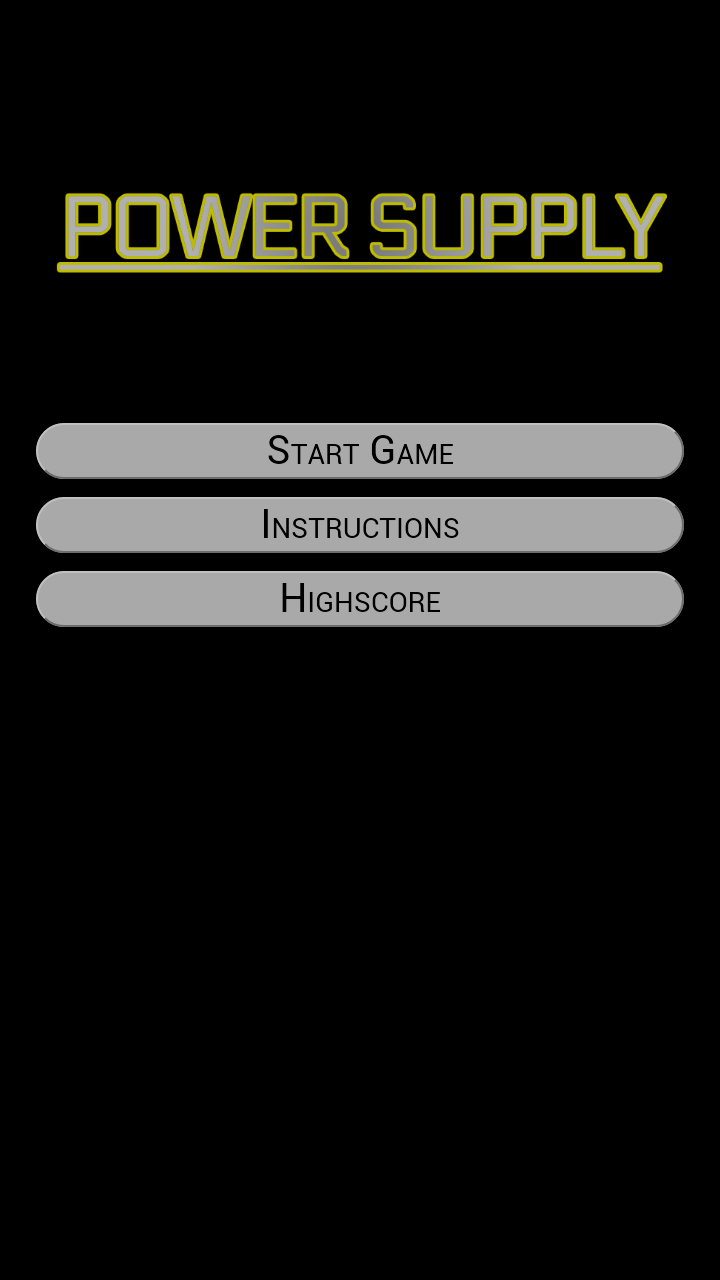
\includegraphics[scale=0.18]{pictures/sprint4-screen/mainmenu}
	}
	\caption{Splash screen when game starts and the game's main menu}
\end{figure}

\begin{figure}[H]
	\centering
	\subfigure{
		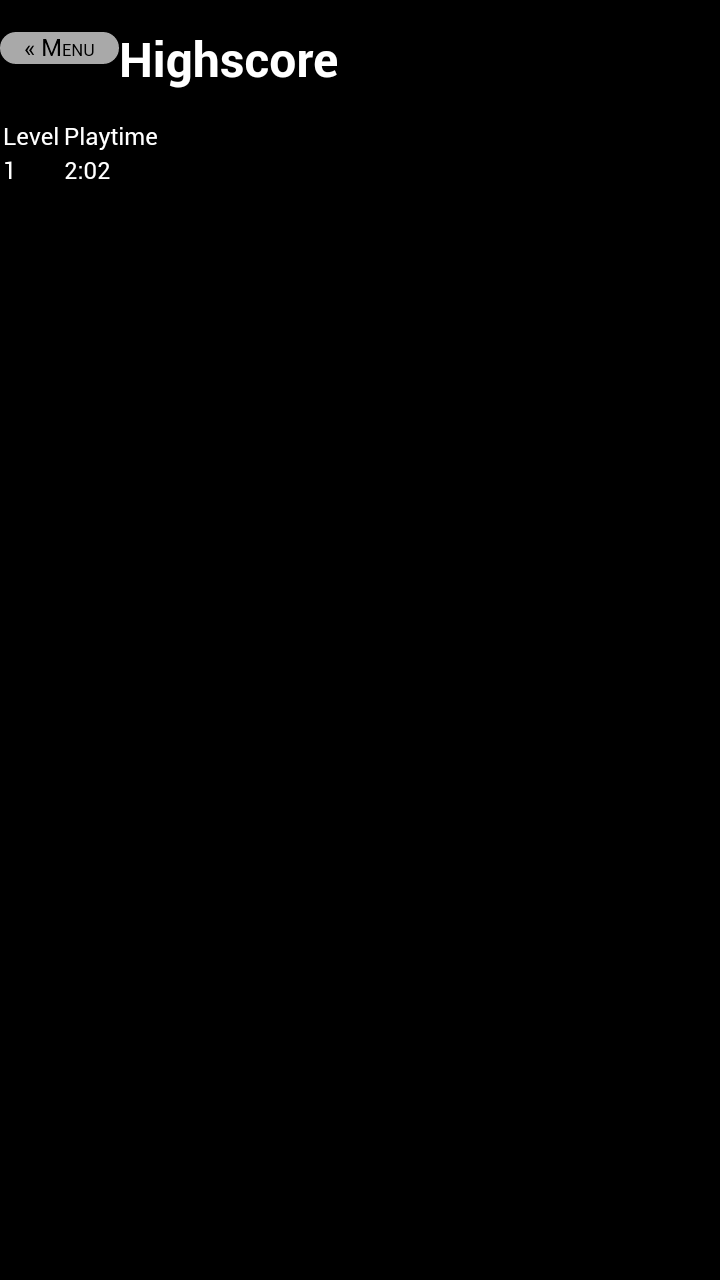
\includegraphics[scale=0.18]{pictures/sprint4-screen/highscore}
	}
	\subfigure{
		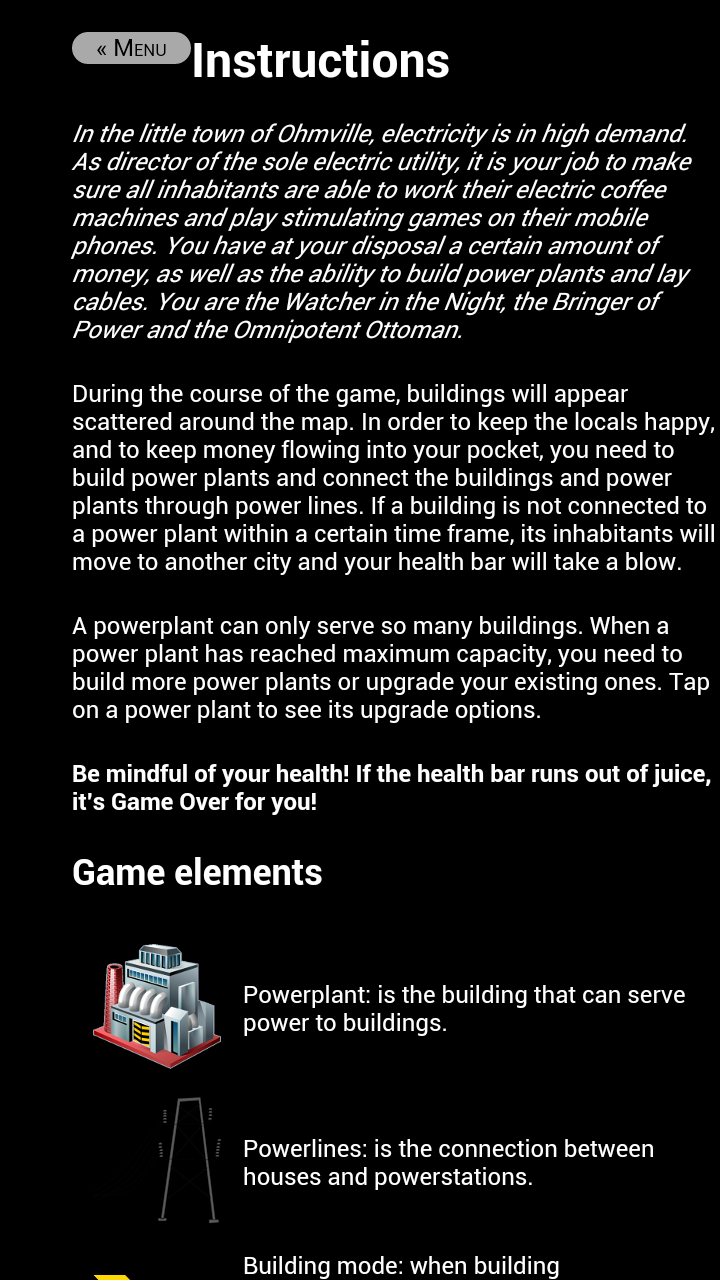
\includegraphics[scale=0.18]{pictures/sprint4-screen/instructions}
	}
	\caption{Highscore and instruction screens}
\end{figure}

\begin{figure}[H]
	\centering
	\subfigure{
		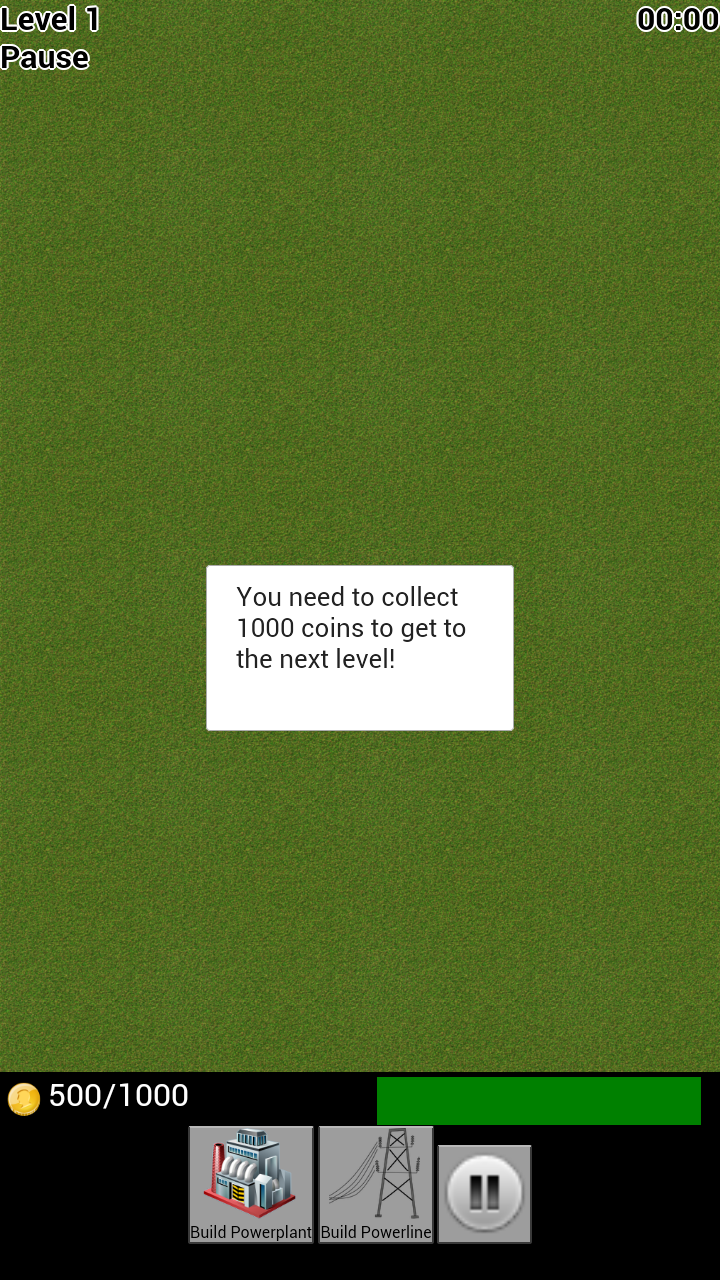
\includegraphics[scale=0.18]{pictures/sprint4-screen/game_start}
	}
	\subfigure{
		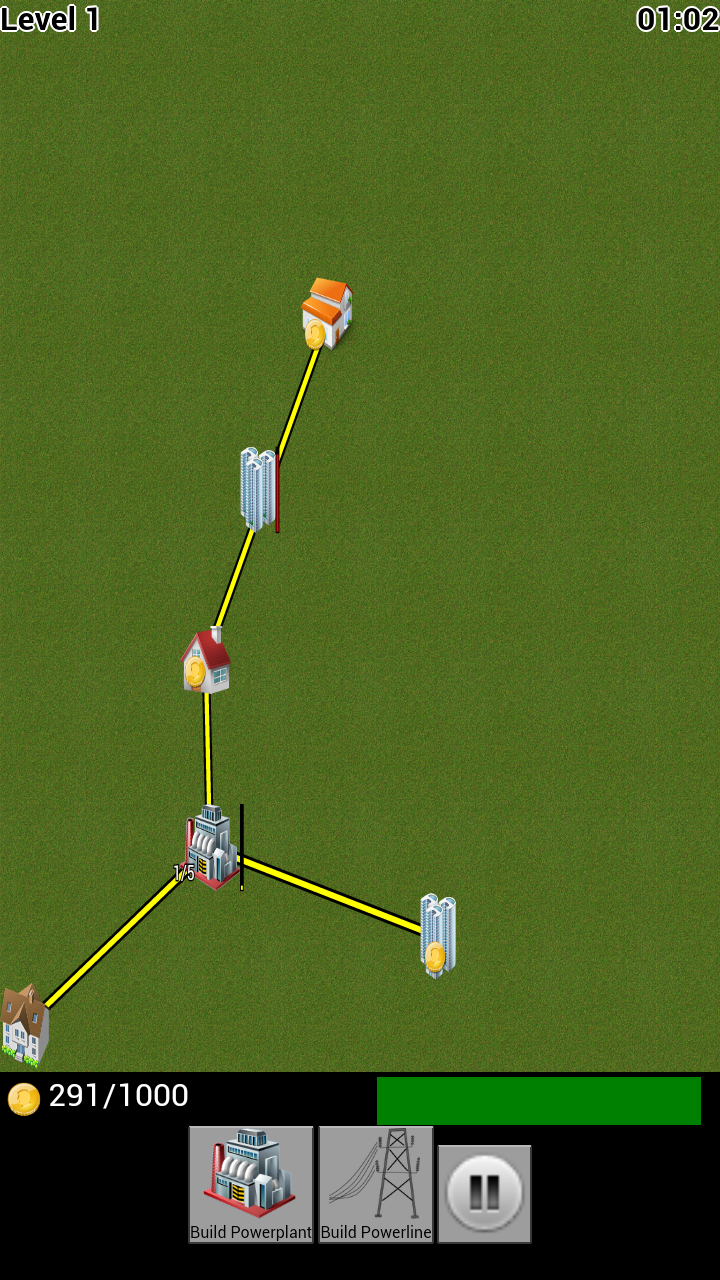
\includegraphics[scale=0.18]{pictures/sprint4-screen/mapoverview}
	}
	\caption{Message when starting a new level and an overview over the map during gameplay}
\end{figure}

\begin{figure}[H]
	\centering
	\subfigure{
		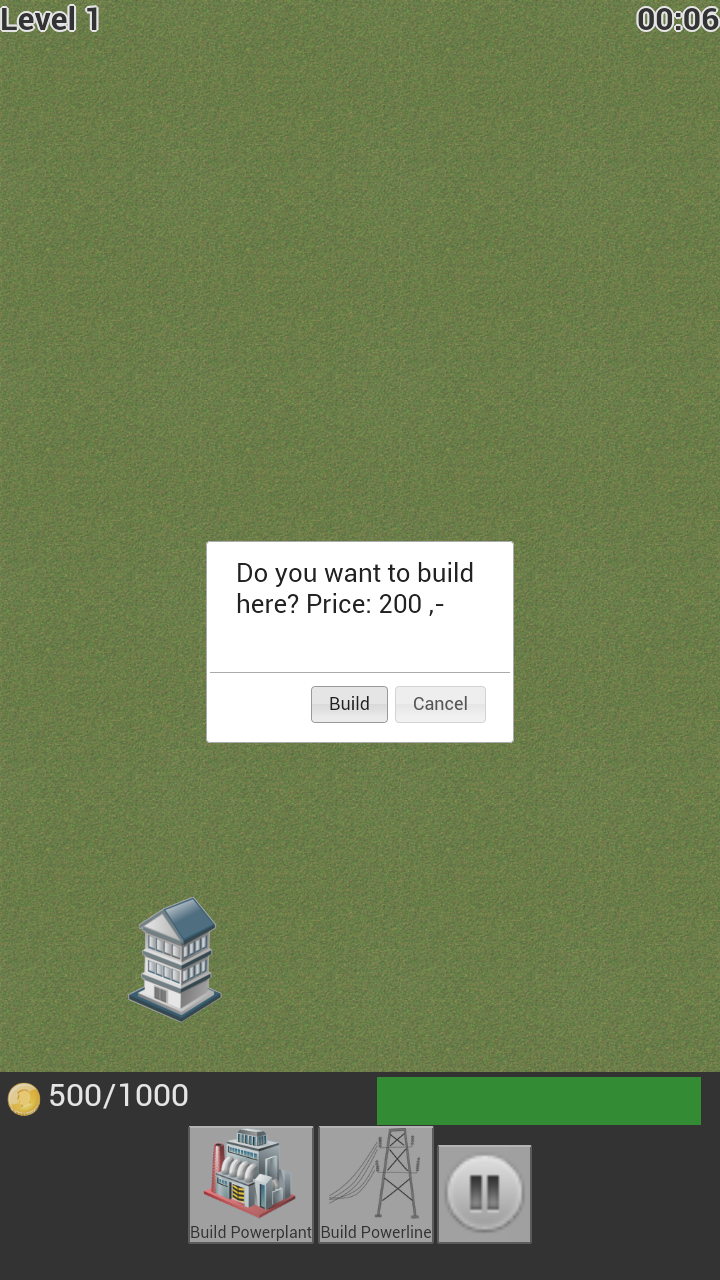
\includegraphics[scale=0.18]{pictures/sprint4-screen/buildpowerplant}
	}
	\subfigure{
		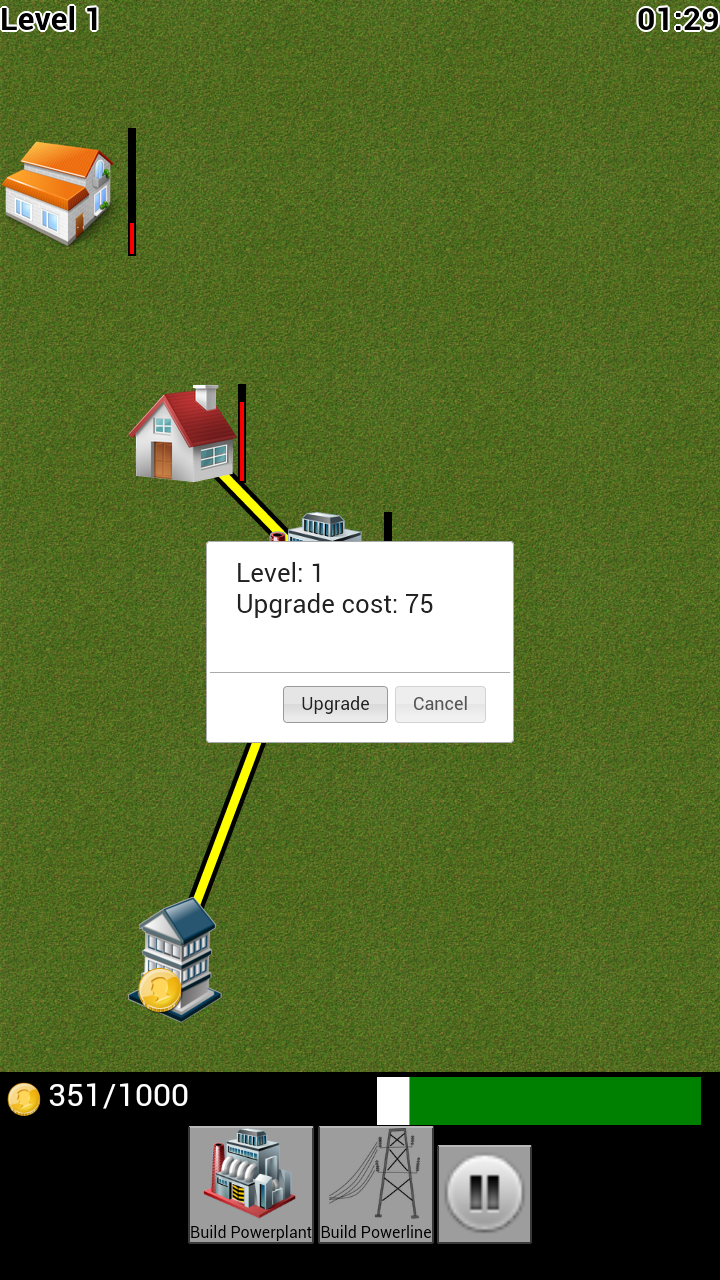
\includegraphics[scale=0.18]{pictures/sprint4-screen/upgradepowerplant}
	}
	\caption{Build and upgrade powerplants}
\end{figure}

\begin{figure}[H]
	\centering
	\subfigure{
		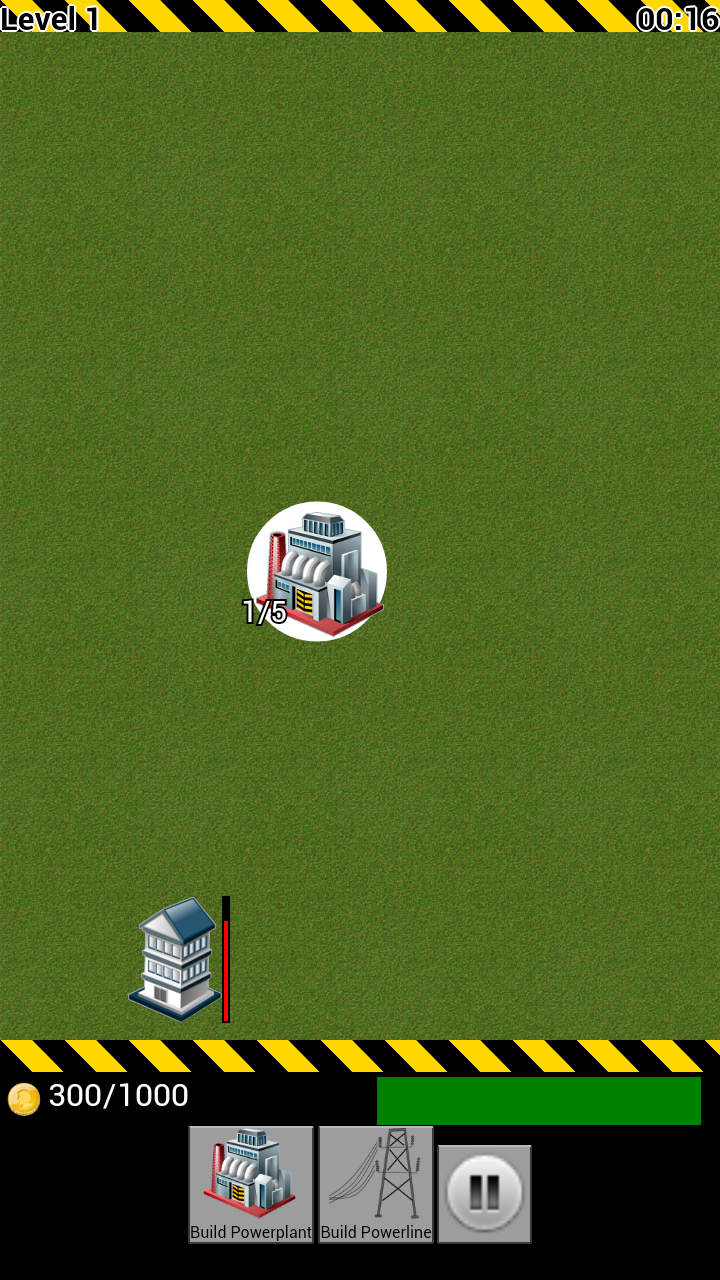
\includegraphics[scale=0.18]{pictures/sprint4-screen/buildpowercable}
	}
	\subfigure{
		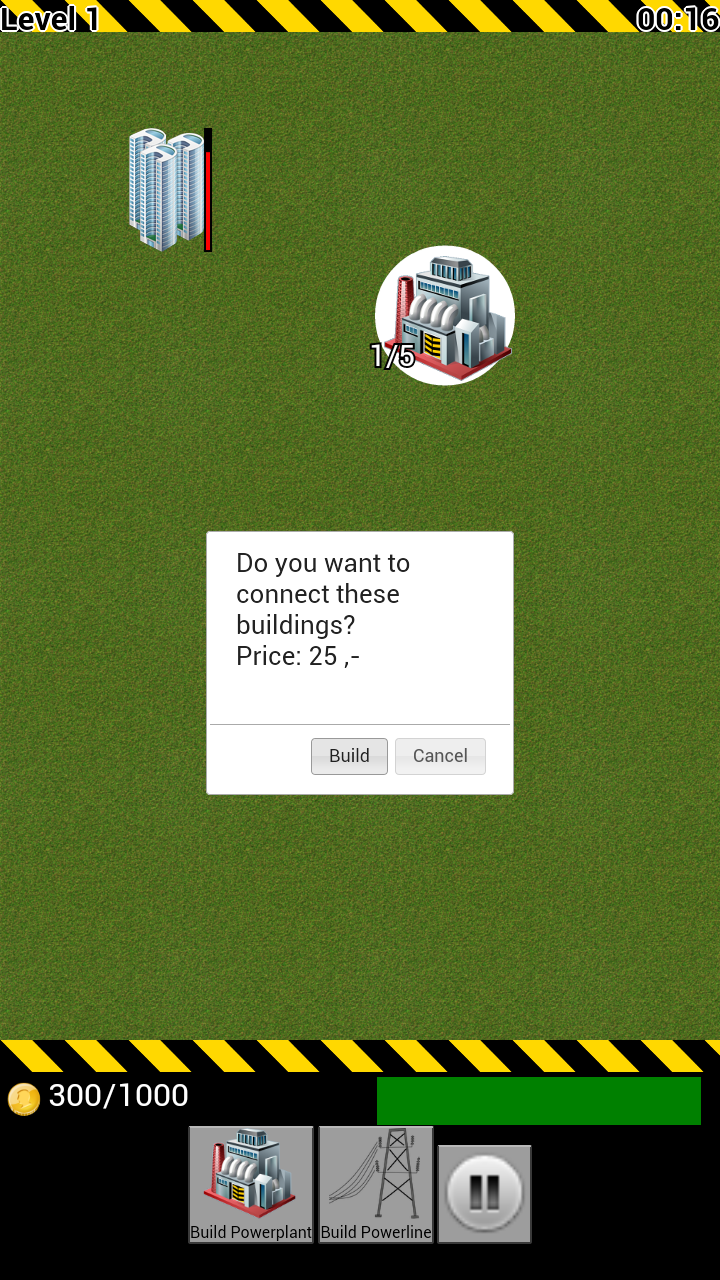
\includegraphics[scale=0.18]{pictures/sprint4-screen/buildpowercable2}
	}
	\caption{Building a power line}
\end{figure}

\begin{figure}[H]
	\centering
	\subfigure{
		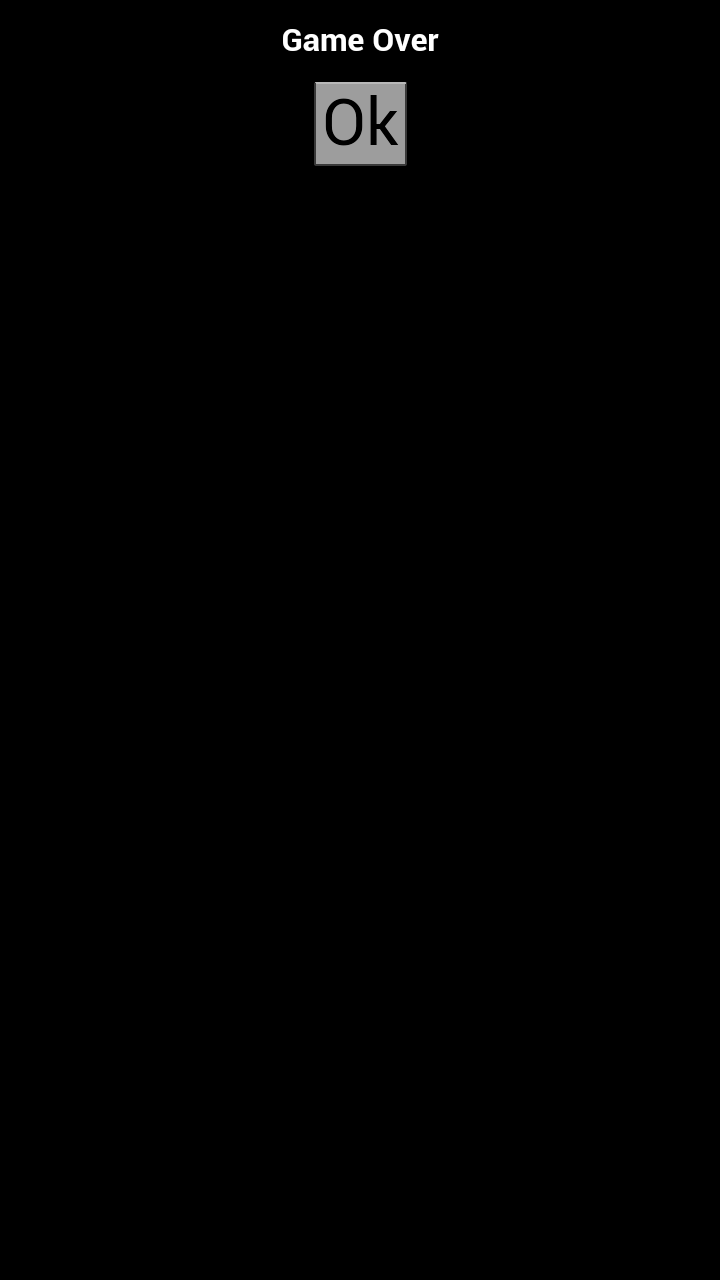
\includegraphics[scale=0.18]{pictures/sprint4-screen/gameover}
	}
	\subfigure{
		\includegraphics[scale=0.18]{pictures/sprint4-screen/victory}
	}
	\caption{Gameover and victory screens}
\end{figure}


\subsection{Redesign and bug fixing}
	
	\subsubsection*{Changes to hud}
		**Made the hud static**
		After receiving feedback from the customer and through observations during the usability test in sprint 3, it was decided that the hud was going to be static, i.e. it was not going to be necessary to move it up in order to build.The two icons for building power plants and power lines were made slightly smaller to not make the screen look cluttered.

	\subsubsection*{Scaling GUI elements on iOS}
		Because of differences in screen resolution and in how different browsers
		render HTML content, some pieces of text and images were too large on iOS
		when compared to how they appeared on Android. These issues are not
		technically challenging, generally speaking, but they are quite
		unpredictable and solving them requires some experimentation. All of the
		known layout problems on iOS were solved during this sprint.

	\subsubsection*{Input handling on iOS}
		Because the iOS and Android browsers handle JavaScript TouchEvents
		differently, we had some problems in making map panning work on both
		platforms. This was a fairly subtle bug which took a lot of time to
		understand, but it was solved in the end.

		It turns out that the screen coordinates of a touch event are stored in
		a list of historical touch events, as suggested by the W3C
		documentation\cite{touchEventDocumentation}, in the Android browser.
		On iOS, however, the correct coordinates are only available directly from
		each individual touch object. In order to make panning work well on both
		platforms, we've chosen to detect which platform the app is running on
		and change its behaviour accordingly.

	\subsubsection*{Changed Game logo}
		We did not know which font was used in the first logo, so we changed it to a new
		and better looking one. 

		\begin{figure}
			\centering
			\includegraphics[scale=0.4]{pictures/logo2.png}
			\caption{Old logo}
		\end{figure}

		\begin{figure}
			\centering
			\includegraphics[scale=0.4]{pictures/newLogo.png}
			\caption{New logo}
		\end{figure}


\subsection{Testing}

	The following test cases were executed at the end of this sprint:

	\definecolor{lightgray}{gray}{0.9}

	\begin{tabular}{| p{3cm} | p{7cm} | p{2cm} |}
		\hline
		\rowcolor{lightgray}
		{\bf Test Case} & {\bf Result} & {\bf Pass/Fail} \\ \hline

		FT-25 High score & Works as expected. & Pass. \\ \hline

		FT-26 Pause Game & If one leaves the game while paused the alert follows to the main menu. In order 
		to get anything done in the main menu one need to press 'Resume', which makes the game continue while 
		the player is in the main menu. It can be intuitive for the player to pause the game before going to 
		the main menu, but in the case of our game this works better by just leaving the game. Otherwise the 
		pause function works. & Partially pass. \\ \hline

		FT-27 Sound Effects & Sound does not work on some devices. & Partially pass. \\ \hline

		FT-28 Exit Game & If the game is left when a level is completed, but before the next level has been 
		entered, the game returns to main menu and the player needs to start at level 1 again. When exiting 
		the game while in playing mode, it works. & Partially pass. \\ \hline



		%FT-32 Power Preservation Tip &  & \\ \hline 
	\end{tabular}

	The following test cases did not pass previous tests and were retested this sprint:

	\begin{tabular}{| p{3cm} | p{7cm} | p{2cm} |}
		\hline
		\rowcolor{lightgray}
		{\bf Test Case} & {\bf Result} & {\bf Pass/Fail} \\ \hline
		
		FT-02 Appearance of buildings & Buildings do not appear on top of each other anymore. & Pass. \\ \hline
		
		FT-05 Build Power Plants & Power Plant are not possible to place on top of other buildings. & Pass. \\ \hline
		
		FT-06 Build Power Lines & There is still no constraints on where power lines can be built as long as it is between two buildings. Otherwise they work. & Partially pass. \\ \hline
		
		FT-20 Damaged Power Lines & Power lines are now possible to fix. & Pass. \\ \hline
	\end{tabular}

	The test cases that are marked with 'partially pass', works mostly as expected, but has some bugs 
	that we will not be able to fix before delivery.

	Other bugs that was were discovered during testing was that if a building or a power plant is placed 
	too far on the right side on the game map, their bar is not visible to the player. Also after having 
	changed the styling of the dialog box for building power lines, it was no longer possible to decline 
	building a power line when asked.

\subsection{Changes to the requirements}

	The fact that buildings should not appear on top of each other has finally been added as a requirement, and an additional sound effect requirement has been added.

	Requirement FR1.3 has been removed. The initial plan was that the player could play any level as long as he or she had completed the previous one, and chose which level to play from a menu of all levels. This would be demanding to implement and in addition the levels do not change character to a great extent, only the parameters are changed, from level to level. Therefore it was decided that we will operate with 'tetris-levels', i.e. the player always starts at level 1 and can enter higher levels by winning all previous levels without loosing. 

	{\bf Changes to version 4 of the requirement specification:} \\
	\begin{tabular}{| p{1.5cm} | p{12cm} |}
		\hline
		\rowcolor{lightgray}
		{\bf FR} & {\bf Change} \\ \hline
		FR1.3 & {\bf \color{red}[REMOVED]}The user should be able to restart any level at any given point of time after start playing. \\ \hline
		FR1.14 & {\bf \color{green}[NEW]} There should be played a sound effect when the player builds a power plant. \\ \hline
		FR2.9 & {\bf \color{green}[NEW]} The houses should not appear on top of each other. \\ \hline
		FR6.14 & {\bf \color{green}[NEW]} The user should be able to click a button, and go into "powerline view mode", where the buildings are not rendered and cannot be interacted with. This is to make it easier to see power lines behind buildings etc. \\ \hline
	\end{tabular}

\subsection{Customer feedback}

\clearpage
\section{Delivery phase}
This is delivery phase

\clearpage
\section{Conclusion and Evaluation}
\section{Evaluation}

In this section we will elaborate on YOUR MOM!

\subsection{Internal Process and Results}

	%(How have you worked together as a team? What have you done 
	%well? What have you not done so well? What would you have done differently? Conflicts that 
	%arose and how these were handled? Did you reach the project goals? What did you learn?)

	In the start of the project we had some problems with the dynamics in the group. 
	All the team members are very different in terms of how we like to work, how we communicate, 
	our personalities as well as our experience with this kind of project. Therefore communication 
	did not go so well and people were unsure of what were expected of them. We managed to solve 
	this problem by discussing the problem and discovered that one of the main problems was that 
	the role allocation and the responsibility had not been present. After we made clear what the 
	responsibility to each role was, many of our problems were solved and we managed to work better 
	as a team.

	In most of the sprints we did not manage to reach the goal of working 20-25 hours a week in 
	average per person. However most of the group members did managed to reach this goal individually 
	for most of the weeks. A lot of voluntary work was the reason that some members struggled to reach 
	this goal. Nevertheless, apart from a few minor ones, we completed the requirements in the specification.

	Several of the risks outlined in section 1.8 Risk Management did occur. We received an incomplete 
	requirement specification from customer and handled this by making a complete specification that 
	was approved by the customer, and all in all this did not affect the start-up of the project too much. 
	Some of the members took part in a lot of voluntary work at, among other places, Samfundet. This was handled 
	by giving specific tasks that could be worked on outside group meeting times, but did still lead to fewer 
	working hours. Other school work also affected the work hours, but we tried to work effectively those hours 
	that were spent on the project.

	Unit tests were unfortunately not written. Although we do understand the importance of them, 
	we felt that we needed one more person on the group to make it possible, because we could not 
	find the time and resources for it with the four of us. On the other hand, the functional
	testing helped discovering a lot of bugs and errors on its own.  
	Device testing or compatibility testing was not performed either. We thought we would have more 
	time at the finishing stage of the project than we ended up having.
	We were however very happy with the execution and feedback from the usability test, which proved 
	to be very useful to us.


\subsection{The Customer and Project Task}

	%(How was the communication with the customer? How did you experience the project assignment?)

	The customer is based in Mosjøen, while the team was in Trondheim. This lead us to having the 
	meetings over Skype and it took us some time to find a good way to make this work. In the beginning 
	we had some trouble finding a good way to show the customer the app and let them interact with it, 
	so that they could give us proper feedback. We provided them with a QR-code that let them install 
	the app on their own phones. This did to a certain extent make up for the fact that we could not 
	be in the same room for a meeting.

	We thought the project task sounded very interesting as it would allow us to learn to make a mobile app, 
	something which none of the team members had done before, but which we wanted to be able to do. Also, 
	the team members enjoy playing games themselves, so making a game proved to be a fun kind of task. 
	We did however feel that the task was a bit vague in the beginning and struggled with finding a good 
	concept for a game concerning the power industry, as neither one of us had any extensive knowledge 
	in this field. However when we had agreed on a concept with the customer and the implementation could 
	start we were able to progress without much uncertainty, and no major changes need to be made to the
	game concept after we had begun the implementation.


\subsection{The Advisor}

	%(How was communication with the advisors? Was the supervision good enough? 
	%How could the course be improved to next year?)

	The advisor was engaged in our project and let us know early on if he thought we were facing difficulties or would be and how to best handle these. He gave us a lot of valuable feedback and quickly responded to questions we had outside of the meetings.

\subsection{Suggestions for Improvements}

	We do not know how much communication there was between the course staff and the customers 
	before the start of the course, but we had the impression that several of the customers that 
	took part in the course for the first time did not know what to expect from the project and 
	what was expected of them. Perhaps providing new customers with more information on what to expect 
	and more opportunities to ask questions before the start of the course would make it easier for 
	them to take part in it.

	The composition of the teams could be based on what fields the student have specialized themselves 
	in and the task given. We felt we had a good balance in our group, but other groups may have had a 
	different experience.

%Annet:

%\subsection{Project}


%\subsubsection*{Communication with the customer}

	



%challenges or difficulties?

%communication supervisor?
%group dynamics and role allocations?
%risks?
%goals met/not met?

%\subsection{(Development) Process}

%scrum?
%hours?
%testing?


%\subsection{Implementation}

%backbone?
%phonegap?
%javascript?

%\subsection{Final product}

\section{Conclusion}
\subsection{Further work}

\newpage
\chapter{References}

\begin{thebibliography}{99}

%% How to write the references:
%% 
%% Title of article
%% URL, etc.
%% Date of access (YY-MM-DD)

\bibitem{helgelandskraft}
	Om Helgelandskraft \\
	\href {http://www.helgelandskraft.no/Om-Helgelandskraft/}{http://www.helgelandskraft.no/Om-Helgelandskraft/} \\
	Date: 03.09.13

\bibitem{stakeholder}
	Stakeholder \\
	\href{http://en.wikipedia.org/wiki/Stakeholder}{http://en.wikipedia.org/wiki/Stakeholder} \\
	Date: 20.09.13

\bibitem{methodology}
	Project Management \\
	\href{http://en.wikipedia.org/wiki/Project_management}{http://en.wikipedia.org/wiki/Project\_management} \\
	Date: 23.09.13

\bibitem{agileMethodology}
	Agile Software Development \\
	\href{http://en.wikipedia.org/wiki/Agile_software_development}{http://en.wikipedia.org/wiki/Agile\_software\_development} \\
	Date: 23.09.13

\bibitem{wikiAgile}
	Agile Software Development \\
	\href {http://en.wikipedia.org/wiki/Agile_software_development}{http://en.wikipedia.org/wiki/Agile\_software\_development} \\
	Date: 23.09.13

\bibitem{wikiScrum}
	Scrum \\ 
	\href{http://no.wikipedia.org/wiki/Scrum}{http://no.wikipedia.org/wiki/Scrum} \\
	Date: 23.09.13

\bibitem{architect}
	Software Architect \\
	\href{http://en.wikipedia.org/wiki/Software_architect}{http://en.wikipedia.org/wiki/Software\_architect} \\
	Date: 24.09.13

\bibitem{wikiWaterfall}
	Waterfall Model \\
	\href {http://en.wikipedia.org/wiki/Waterfall_model}{http://en.wikipedia.org/wiki/Waterfall\_model} \\
	Date: 18.09.13

\bibitem{techtargetWaterfall}
	Waterfall Model \\
	\href {http://searchsoftwarequality.techtarget.com/definition/waterfall-model}{http://searchsoftwarequality.techtarget.com/definition/waterfall-model} \\
	Date: 18.09.13

\bibitem{statkraftVannkraft}
	Vannkraft kort forklart \\
	\href {http://www.statkraft.no/energikilder/vannkraft/vannkraft-kort-forklart/}{http://www.statkraft.no/energikilder/vannkraft/vannkraft-kort-forklart/} \\
	Date: 04.09.13

\bibitem{wikiCMS}
	Construction and management simulation \\
	\href {http://en.wikipedia.org/wiki/Construction_and_management_simulation}{http://en.wikipedia.org/wiki/Construction\_and\_management\_simulation} \\
	Date: 04.09.13

\bibitem{megapolis}
	Megapolis \\
	\href {https://play.google.com/store/apps/details?id=com.socialquantum.acityint}{https://play.google.com/store/apps/details?id=com.socialquantum.acityint} \\
	Date: 04.11.13

\bibitem{android}
	Android (OS)\newline
	\href {http://en.wikipedia.org/wiki/Android\_(operating_system)}{en.wikipedia.org/wiki/Android\_(operating\_system)}\newline
	Date: 04.09.13

\bibitem{ios}
	iOS\newline
	\href {http://en.wikipedia.org/wiki/IOS}{en.wikipedia.org/wiki/IOS}\newline
	Date: 04.09.13

\bibitem{iosCost}
	Android (OS)\newline
	\href {https://developer.apple.com/programs/ios/}{developer.apple.com/programs/ios/}\newline
	Date: 09.11.13

\bibitem{usecaseUML}
	UML Use Case Diagrams: Tips and FAQ
	\href {http://www.andrew.cmu.edu/course/90-754/umlucdfaq.html}{http://www.andrew.cmu.edu/course/90-754/umlucdfaq.html}
	Date: 03.10.13

\bibitem{phonegapFAQ}
	Phonegap FAQ\newline
	\href {http://phonegap.com/about/faq/}{phonegap.com/about/faq/}\newline
	Date: 04.09.13

\bibitem{phonegapAbout}
	Phonegap About \\
	\href{http://phonegap.com/about/}{http://phonegap.com/about/} \\
	Date: 04.09.13

\bibitem{backbone}
	Backbone.js \\
	\href{http://backbonejs.org/}{http://backbonejs.org/} \\
	Date: 05.09.13

\bibitem{jasmine}
	Jasmine \\ 
	\href{http://pivotal.github.io/jasmine/}{http://pivotal.github.io/jasmine/} \\
	Date: 05.09.13

\bibitem{coronaSDK}
	Corona SDK\newline
	\href {http://www.coronalabs.com/products/corona-sdk/}{www.coronalabs.com/products/corona-sdk/}\newline
	Date: 04.09.13

\bibitem{github}
	Github Website\\
	\href{https://github.com/}{https://github.com/} \\
	Date: 07.09.13

\bibitem{githubPage}
	Github \\
	\href{http://en.wikipedia.org/wiki/GitHub}{http://en.wikipedia.org/wiki/GitHub} \\
	Date: 07.09.13

\bibitem{trello}
	Trello \\
	\href{https://trello.com/}{https://trello.com/} \\
	Date: 07.09.13

\bibitem{trelloPage}
	Trello \\
	\href{http://en.wikipedia.org/wiki/Trello}{http://en.wikipedia.org/wiki/Trello} \\
	Date: 07.09.13

\bibitem{agileZen}
	AgileZen \\
	\href{http://www.agilezen.com/}{http://www.agilezen.com/} \\
	Date: 07.09.13

\bibitem{drive}
	Google Drive \\
	\href{https://drive.google.com}{https://drive.google.com} \\
	Date: 10.09.13

\bibitem{dropbox}
	Dropbox \\
	\href{https://www.dropbox.com/home}{https://www.dropbox.com/home} \\
	Date: 11.09.13

\bibitem{gameConcept}
	Game Concept\newline
	\href {en.wikipedia.org/wiki/Game\_development#Development\_process}{en.wikipedia.org/wiki/Game\_development\#Development\_process}\newline
	Date: 12.10.13

\bibitem{functionalRequirement}
	Functional Requirement \\
	\href{http://en.wikipedia.org/wiki/Functional_requirement}{http://en.wikipedia.org/wiki/Functional\_requirement} \\
	Date: 02.10.13

\bibitem{nonFunctionalRequirement}
	Non-Functional Requirement \\
	\href{http://en.wikipedia.org/wiki/Non-functional_requirement}{http://en.wikipedia.org/wiki/Non-functional_requirement} \\
	Date: 02.10.13

\bibitem{qualityAttribute}
	Quality Attribute \\
	\href{http://www.ece.ubc.ca/~matei/EECE417/BASS/ch04lev1sec3.html}{http://www.ece.ubc.ca/~matei/EECE417/BASS/ch04lev1sec3.html} \\
	Date: 04.10.13

\bibitem{attributes}
	Quality Attribute Scenarios in Practice \\ 
	\href{http://www.ece.ubc.ca/~matei/EECE417/BASS/ch04lev1sec4.html}{ttp://www.ece.ubc.ca/~matei/EECE417/BASS/ch04lev1sec4.html} \\
	Date: 05.10.13

\bibitem{architecturalTactics}
	Introduction to Tactics \newline
	\url {http://www.ece.ubc.ca/~matei/EECE417/BASS/ch05lev1sec1.html}{http://www.ece.ubc.ca/~matei/EECE417/BASS/ch05lev1sec1.html} \newline
	Date: 02.10.13

\bibitem{estimation}
	Agile Q\&A – GreenHopper Time Estimates with Sub-Tasks \\
	\href{http://blogs.atlassian.com/2012/09/agile-qa-greenhopper-time-estimates-with-sub-tasks/}{http://blogs.atlassian.com/2012/09/agile-qa-greenhopper-time-estimates-with-sub-tasks/} \\
	Date: 28.10.13

\bibitem{mvp}
	Model-View-Presenter\newline
	\href {http://backbonejs.org/\#FAQ-mvc}{http://backbonejs.org/\#FAQ-mvc}\newline
	Date: 03.10.13

\bibitem{pldTheory}
	Point Line Distance Theory\newline
	\href {http://math.stackexchange.com/a/322836}{http://math.stackexchange.com/a/322836}\newline
	Date: 26.10.13

\bibitem{pldCode}
	Point Line Distance Code\newline
	\href {http://stackoverflow.com/a/1501725}{http://stackoverflow.com/a/1501725}\newline
	Date: 26.10.13

\bibitem{whiteblacboxtesting}
	Differences Between Black Box Testing and White Box Testing \\
	\href {http://softwaretestingfundamentals.com/differences-between-black-box-testing-and-white-box-testing/}{http://softwaretestingfundamentals.com/differences-between-black-box-testing-and-white-box-testing/} \\
	Date: 10.09.13

\bibitem{unitTesting}
	Unit Testing \\
	\href {http://en.wikipedia.org/wiki/Unit_testing}{http://en.wikipedia.org/wiki/Unit\_testing} \\
	Date: 10.09.13

\bibitem{functionalTesting}
	Functional Testing \\
	\href {http://en.wikipedia.org/wiki/Functional_testing}{http://en.wikipedia.org/wiki/Functional\_testing} \\
	Date: 10.09.13

\bibitem{usabilityTesting}
	Usability Testing \\
	\href {http://en.wikipedia.org/wiki/Usability_testing}{http://en.wikipedia.org/wiki/Usability\_testing} \\
	Date: 10.09.13

\bibitem{compatibilityTesting}
	Compatibility Testing \\
	\href {http://en.wikipedia.org/wiki/Compatibility_testing}{http://en.wikipedia.org/wiki/Compatibility\_testing} \\
	Date: 10.09.13

\bibitem{integrationTesting}
	Integration Testing \\
	\href{http://en.wikipedia.org/wiki/Integration_testing}{http://en.wikipedia.org/wiki/Integration\_testing} \\
	Date: 10.09.13

\bibitem{ISOusability}
	ISO 9241-11 \\
	\href {http://en.wikipedia.org/wiki/ISO_9241#ISO_9241-11}{http://en.wikipedia.org/wiki/ISO\_9241\#ISO\_9241-11} \\
	Date: 17.10.13

\bibitem{numberOfUsers}
	Why you only need to test with 5 users \\
	\href {http://www.nngroup.com/articles/why-you-only-need-to-test-with-5-users/}{http://www.nngroup.com/articles/why-you-only-need-to-test-with-5-users/} \\
	Date: 17.10.13

\bibitem{sus}
	System Usability Scale \\
	\href {http://www.measuringusability.com/sus.php}{http://www.measuringusability.com/sus.php} \\
	Date: 21.10.13 

\bibitem{evaluationSheet}
	Game Evaluation Sheet \\
	\href {http://thebiggamehunter.com/game-evaluation-sheet/}{http://thebiggamehunter.com/game-evaluation-sheet/} \\
	Date: 21.10.13
\end{thebibliography}
\clearpage

\section*{Appendices}
\appendix
\chapter{Glossary}

\clearpage
heihei
\clearpage
\chapter{Templates}
\label{chap:templates}

\clearpage

\section{Customer Meeting Invite}

\begin{itemize}
	\item Date and Time:
	\item Room/skype account:
	\item Agenda:
\end{itemize}

\section{Customer Meeting Minutes}

\begin{tabular}{| p{3cm} | p{9cm} |}
	\hline
	\rowcolor{gray}
	\multicolumn{2}{|c|}{\Large \bf Meeting Minutes - Customer Meeting} \\ \hline
	Date and time: & dd.mm,  hh.mm - hh.mm \\ \hline
	Room or skype username: &  \\ \hline
	Present: &  \\ \hline
	Not present: &  \\ \hline
	Author: &  \\ \hline
	Purpose: &  \\ \hline
\end{tabular}

\begin{tabular}{| p{2,6cm} | p{4,5cm} | p{4,5cm} |}
	\hline
	\rowcolor{gray}
	\multicolumn{3}{|c|}{\Large \bf Agenda} \\ \hline
	{\bf Topic} & {\bf Discussion} & {\bf Action (TODO)} \\ \hline
	& & \\ \hline
	& & \\ \hline
\end{tabular}

\section{Supervisor Meeting Invite}

\begin{itemize}
	\item Date and Time:
	\item Room:
	\item Agenda:
\end{itemize}

\section{Supervisor Meeting Minutes}
\begin{tabular}{| p{3cm} | p{9cm} |}
	\hline
	\rowcolor{gray}
	\multicolumn{2}{|c|}{\Large \bf Meeting Minutes - Supervisor Meeting} \\ \hline
	Date and time: & dd.mm,  hh.mm - hh.mm \\ \hline
	Room: &  \\ \hline
	Present: &  \\ \hline
	Not present: &  \\ \hline
	Author: &  \\ \hline
	Purpose: &  \\ \hline
\end{tabular}

\begin{tabular}{| p{2,6cm} | p{4,5cm} | p{4,5cm} |}
	\hline
	\rowcolor{gray}
	\multicolumn{3}{|c|}{\Large \bf Agenda} \\ \hline
	{\bf Topic} & {\bf Discussion} & {\bf Action (TODO)} \\ \hline
	& & \\ \hline
	& & \\ \hline
\end{tabular}

\section{Template for Time Accounting}

\begin{figure}[H]
	\includegraphics[width=\textwidth]{pictures/timetable.png}
	\caption{Timetable}
\end{figure}
\clearpage
\chapter{Standards}
\clearpage
\section{Test Cases}

\begin{table}[H]
\centering
	\begin{tabular}{ l | p{8cm} }
		\hline
		{\bf Item} & {\bf Description} \\ \hline
		Name & Map and Navigation \\ 
		Test Id & FT-01 \\ 
		Feature to be tested & That user should be able to see a small part of the game map and be able to navigate around it.\\ 
		Requirement & FR6.1 and FR6.2 \\ 
		Pre-conditions & None \\ 
		Steps of Execution & 1. Drag a finger over the screen. \\
		& 2. Try to navigate outside the game map. \\
		Expected result & 1. The screen will move across the map in the opposite direction of the finger.\\ 
		& 2. Nothing happens. \\
	\end{tabular}
	\caption{Functional test 1}
\end{table}

\begin{table}[H]
\centering
	\begin{tabular}{ l | p{8cm} }
		\hline
		{\bf Item} & {\bf Description} \\ \hline
		Name & Appearance of buildings \\ 
		Test Id & FT-02 \\ 
		Feature to be tested & That buildings appear around the map at arbitrary intervals and locations. \\ 
		Requirement & FR2.1 \\ 
		Pre-conditions & FT-01 \\ 
		Steps of Execution & 1. Observe that buildings appear around the map at arbitrary intervals and locations.\\ 
		Expected result & 1. Buildings appear around the map at arbitrary intervals and locations at a satisfying rate.\\ 
	\end{tabular}
	\caption{Functional test 2}
\end{table}

\begin{table}[H]
\centering
	\begin{tabular}{ l | p{8cm} }
		\hline
		{\bf Item} & {\bf Description} \\ \hline
		Name & Zooming \\ 
		Test Id & FT-03 \\ 
		Feature to be tested & The shifting between zoomed-out and zoomed-in screens. \\ 
		Requirement & FR6.4 \\ 
		Pre-conditions & FT-01 \\ 
		Steps of Execution & 1. Double tap the screen in zoomed-in mode.\\ 
		& 2. Double tap the screen in zoomed-out mode. \\
		Expected result & 1. The screen will show the whole game map. \\
		& 2. The screen will show the part of the game map where the player tapped the screen. \\
	\end{tabular}
	\caption{Functional test 3}
\end{table}

\begin{table}[H]
\centering
	\begin{tabular}{ l | p{8cm} }
		\hline
		{\bf Item} & {\bf Description} \\ \hline
		Name & Main Menu \\ 
		Test Id & FT-04 \\ 
		Feature to be tested & That the buttons in the main menu directs to the correct pages. \\ 
		Requirement & FR1.1, FR6.7 ?Highscore?, ?Start Game? \\ 
		Pre-conditions & FT-01 \\ 
		Steps of Execution & 1. Tap the 'New Game' button. \\
		& 2. Tap the 'Instructions' button. \\
		& 3. Tap the 'Highscore' button. \\
		Expected result & 1. A new game is started. \\
		& 2. The page showing the game instructions is shown. \\
		& 3. The page showing the high score is shown. \\
	\end{tabular}
	\caption{Functional test 4}
\end{table}

\begin{table}[H]
\centering
	\begin{tabular}{ l | p{8cm} }
		\hline
		{\bf Item} & {\bf Description} \\ \hline
		Name & Build Power Plants \\ 
		Test Id & FT-05 \\ 
		Feature to be tested & That it is possible to buy and place power plants on the game map. \\ 
		Requirement & FR2.2, FR6.8 \\ 
		Pre-conditions & FT-01. First the player can afford a Power Plant, subsequently the player can not afford a Power Plant. \\
		Steps of Execution & 1. Drag the build menu into view. \\ 
		& 2. Tap the power plant icon. \\
		& 3. Tap somewhere on the map where a power plant can not be placed e.g. a building. \\
		& 4. Tap an emty area on the map. \\
		& 5. Tap 'OK'. \\
		& 6. Repeat, but tap 'Cancel'. \\
		Expected result & 2.1 If player has enough money the game is set to building mode. \\
		& 2.2 If player does not have enough money, information is displayed. \\
		& 3. Nothing happens. \\ 
		& 4. The player is asked to either buy or cancel. \\
		& 5. The power plant is placed on the indicated spot and the players amount of money is reduced. \\
		& 6. Leave building mode. \\
	\end{tabular}
	\caption{Functional test 5}
\end{table}

\begin{table}[H]
\centering
	\begin{tabular}{ l | p{8cm} }
		\hline
		{\bf Item} & {\bf Description} \\ \hline
		Name & Build Power Lines \\ 
		Test Id & FT-06 \\ 
		Feature to be tested &  That it is possible to buy power cables and connect buildings and power plants. \\ 
		Requirement & FR2.3, FR5.2, FR6.8 \\ 
		Pre-conditions & FT-02, FT-05. First the player can afford a Power Plant, subsequently the player can not afford a Power Plant.\\ 
		Steps of Execution & 1. Drag the build menu into view. \\
		& 2. Tap the power cable icon. \\
		& 3. Tap somewhere on the map where a power cable can not be placed. \\
		& 4. Tap a Power Plant, then tap a building. \\
		& 5. Observe the player's money bag. \\
		& 6. Try to connect an already connected building to another power plant. \\
		& 7. Connect a building and a power plant, and try to let the power cable cross another power cable. \\
		Expected result & 2.1 If player has enough money the game is set to building mode. \\
		& 2.2 If player does not have enough money, information is displayed. \\
		& 3. Nothing happens. \\
		& 4. The two are connected by a cable. \\
		& 5. The power cable cost some amount of money proportional to the length. \\
		& 6. Should not be allowed. \\
		& 7. Should not be allowed. \\
	\end{tabular}
	\caption{Functional test 6}
\end{table}

\begin{table}[H]
\centering
	\begin{tabular}{ l | p{8cm} }
		\hline
		{\bf Item} & {\bf Description} \\ \hline
		Name & Upgrade Power Plant\\ 
		Test Id & FT-07 \\ 
		Feature to be tested & That it is possible to upgrade a power plant. \\ 
		Requirement & FR2.4, FR5.3, FR6.3 \\ 
		Pre-conditions & FT-05. First the player does not have enough money. Subsequently the player does have enough money. \\ 
		Steps of Execution & 1. Tap a power plant. \\ 
		& 2. Choose 'Upgrade Power Plant'. \\
		& 3. Choose "Upgrade" from the pop up. \\
		Expected result & 1. An information box about the cost of upgrading and the effects of upgrading is displayed. \\
		& 2. The system asks whether to 'Upgrade' or 'Cancel'. \\
		& 3. When not having enough money the system gives accordant feedback. \\
		& 3. When having enough money the system reduces the players amount of money by the cost of the power plant, and upgrades the power plant. This is displayed on the power plant. \\
	\end{tabular}
	\caption{Functional test 7}
\end{table}

\begin{table}[H]
\centering
	\begin{tabular}{ l | p{8cm} }
		\hline
		{\bf Item} & {\bf Description} \\ \hline
		Name & Information on Buildings and Power Plants \\ 
		Test Id & FT-08 \\ 
		Feature to be tested & That information specific to the building appears when tapping them. \\ 
		Requirement & FR2.8 \\ 
		Pre-conditions & FT-02, FT-05, FT-07. \\ 
		Steps of Execution & 1. Tap different kinds of buildings. \\
		& 2. Tap a Power Plant that has not been upgraded. \\
		& 3. Tap an upgraded Power Plant. \\
		Expected result & 1. Information on how much power the building needs is displayed. \\
		& 2. Information on which level of upgrade the player can upgrade to is displayed as well as information on how much it costs and what it does for the power plant. \\
	\end{tabular}
	\caption{Functional test 8}
\end{table}

\begin{table}[H]
\centering
	\begin{tabular}{ l | p{8cm} }
		\hline
		{\bf Item} & {\bf Description} \\ \hline
		Name & Building Mode \\ 
		Test Id & FT-09 \\ 
		Feature to be tested & That the game is set in "Building Mode" when building power plants or power cables. \\ 
		Requirement & FR6.9 \\ 
		Pre-conditions & FT-06 \\ 
		Steps of Execution & 1. Drag the build menu into view. \\ 
		& 2. Tap the Power Plant. \\
		& 3. Tap an emty location on the screen. \\
		& 4. Tap 'Cancel'. \\
		& 5. Tap the Power Cable. \\
		& 6. Tap an emty location on the screen. \\
		& 7. Tap 'Cancel'. \\
		Expected result & 2. Building Mode is avtivated. \\ 
		& 4. Building Mode is ended. \\
		& 5. Building Mode is activated. \\
		& 7. Building Mode is ended. \\
	\end{tabular}
	\caption{Functional test 9}
\end{table}

\begin{table}[H]
\centering
	\begin{tabular}{ l | p{8cm} }
		\hline
		{\bf Item} & {\bf Description} \\ \hline
		Name & Tilting \\ 
		Test Id & FT-10 \\ 
		Feature to be tested & That the screen picture is not tiltet when the phone is tilted. \\ 
		Requirement & FR1.12 \\ 
		Pre-conditions & FT-01 \\ 
		Steps of Execution & 1. Tilt the phone. \\ 
		Expected result & The screen picture stays in place. \\ 
	\end{tabular}
	\caption{Functional test 10}
\end{table}

\begin{table}[H]
\centering
	\begin{tabular}{ l | p{8cm} }
		\hline
		{\bf Item} & {\bf Description} \\ \hline
		Name & Collect money \\ 
		Test Id & FT-11 \\ 
		Feature to be tested & That it is possible to collect money from different buildings connected to the power plants at regular intervals. \\
		Requirement & FR3.4, FR5.1 \\ 
		Pre-conditions & FT-06. \\ 
		Steps of Execution & 1. Buildings are ready to pay for their electricity. \\
		& 2. Tap a certain type of building. \\ 
		& 3. Repeat step 2 for all different buildings. \\
		Expected result & 1. The building has a collect money sign. \\
		& 2. The players money is updated and the sign disappears. \\
		& 3. The buildings pay different amounts of money depending on their type. \\
	\end{tabular}
	\caption{Functional test 11}
\end{table}

\begin{table}[H]
\centering
	\begin{tabular}{ l | p{8cm} }
		\hline
		{\bf Item} & {\bf Description} \\ \hline
		Name & No Power and Health Bar \\ 
		Test Id & FT-12 \\ 
		Feature to be tested & That it is visible that a building has not been supplied with power for a while. And that eventually the house dissapears and the player's health score decreases. \\
		Requirement & FR3.6, FR6.10 \\ 
		Pre-conditions & FT-06 \\ 
		Steps of Execution &  1. Observe a building that is not connected to a Power Plant. \\ 
		& 2. Observe the building when the time limit has been reached. \\
		& 3. Observe the Health Bar. \\
		& 4. Connect an unconnected house to a power plant. \\
		Expected result & 1 A bar placed next to the building slowly decreases. \\
		& 2. The house disappears, when the bar is emty. \\
		& 3. The Health Bar decreases by a certain amount. \\
		& 4. The building's bar disappears. \\
	\end{tabular}
	\caption{Functional test 12}
\end{table}

\begin{table}[H]
\centering
	\begin{tabular}{ l | p{8cm} }
		\hline
		{\bf Item} & {\bf Description} \\ \hline
		Name & Game Over \\ 
		Test Id & FT-13 \\ 
		Feature to be tested & That the game is over when the health score reaches zero. \\ 
		Requirement & FR4.2 \\ 
		Pre-conditions & FT-13 \\ 
		Steps of Execution & 1. Let several buildings not get power. \\ 
		& 2. Let the health score decrease to zero. \\
		& 3. Tap 'OK'. \\
		& 4. Tap 'New Game'. \\
		Expected result & 1. The health score is decreasing as houses not supllied with power disappears. \\
		& 2. The "Game Over" page is displayed, with an 'OK' button. \\
		& 3. The main menu page is displayed. \\
		& 4. A new game is started. \\
	\end{tabular}
	\caption{Functional test 13}
\end{table}

\begin{table}[H]
\centering
	\begin{tabular}{ l | p{8cm} }
		\hline
		{\bf Item} & {\bf Description} \\ \hline
		Name & Win Game \\ 
		Test Id & FT-14 \\ 
		Feature to be tested & That it is possible to win the game \\ 
		Requirement & FR4.6 \\ 
		Pre-conditions & \\ 
		Steps of Execution &  \\ 
		Expected result & \\ 
	\end{tabular}
	\caption{Functional test 14}
\end{table}

\begin{table}[H]
\centering
	\begin{tabular}{ l | p{8cm} }
		\hline
		{\bf Item} & {\bf Description} \\ \hline
		Name & Exit Game \\ 
		Test Id & FT-15 \\ 
		Feature to be tested & Test that the game is paused when exiting the game. \\ 
		Requirement & FR1.2 \\ 
		Pre-conditions & FT-04. \\ 
		Steps of Execution & 1. Leave the game by tapping the home button on the phone. \\
		& 2. Open the game app. \\
		& 3. Tap 'Load Game'. \\
		Expected result & 3. The game is paused at the point where it was left. \\  
	\end{tabular}
	\caption{Functional test 15}
\end{table}

\begin{table}[H]
\centering
	\begin{tabular}{ l | p{8cm} }
		\hline
		{\bf Item} & {\bf Description} \\ \hline
		Name & Limited Power \\ 
		Test Id & FT-16 \\ 
		Feature to be tested & Test that the amount of power avaialbe to the player is limited, and the effects of upgrading. \\ 
		Requirement & FR2.5 \\ 
		Pre-conditions & FT-06, FT-08\\ 
		Steps of Execution & 1. Connect a power plant and a building with a power cable. \\
		& 2. Repeat step 1 for other buildings, using the same power plant, until and after the power bar is emty. \\
		& 3. Upgrade the power plant. \\
		& 5. Connect the power plant to another building. \\
		Expected result & 2. The power plant is not able to serve more buildings and a splash screen will appear. \\ 
		& 4. The power bar will gain more content and the power plant is now able to serve more power. \\
		& 5. This is now possible, no error message appears. \\
	\end{tabular}
	\caption{Functional test 16}
\end{table}

\begin{table}[H]
\centering
	\begin{tabular}{ l | p{8cm} }
		\hline
		{\bf Item} & {\bf Description} \\ \hline
		Name & Remove Power Cables \\ 
		Test Id & FT-17 \\ 
		Feature to be tested & That it is possible to remove Power Cables from the map. \\ 
		Requirement & FR2.6 \\ 
		Pre-conditions & FT-06 \\ 
		Steps of Execution &  \\ 
		Expected result & \\ 
	\end{tabular}
	\caption{Functional test 17}
\end{table}

\begin{table}[H]
\centering
	\begin{tabular}{ l | p{8cm} }
		\hline
		{\bf Item} & {\bf Description} \\ \hline
		Name & Number of Power Plants \\ 
		Test Id & FT-18 \\ 
		Feature to be tested & That it is only possible to build a certain amount of Power Plants specific to the level. \\ 
		Requirement & FR2.7 \\ 
		Pre-conditions & FT-05, FT-14. \\ 
		Steps of Execution & 1. Build a power plant. \\ 
		& 2. Build power plants until the number of power plants reaches 0, and try beyond that. \\
		Expected result & 1. The number on the power plant in the hud (Initially toatal number of power plant one can build.) decreases by one. \\
		& 2. When the number reaches 0 and one tries to build another one, an error message is displayed. \\
	\end{tabular}
	\caption{Functional test 18}
\end{table}

\begin{table}[H]
\centering
	\begin{tabular}{ l | p{8cm} }
		\hline
		{\bf Item} & {\bf Description} \\ \hline
		Name & Different Buildings \\ 
		Test Id & FT-19 \\ 
		Feature to be tested & There are different buildings and they have different power requirements. \\ 
		Requirement & FR3.3 \\ 
		Pre-conditions & FT-06, FT-08 \\ 
		Steps of Execution & 1. Connect a power plant to the smallest type of building. \\
		& 2. Repeat for the five other types of buildings. \\
		Expected result & 1. The power bar on the power station decreases by a small amount. \\
		& 2. The bigger the building is the more the power bar decreases. \\
	\end{tabular}
	\caption{Functional test 19}
\end{table}

\begin{table}[H]
\centering
	\begin{tabular}{ l | p{8cm} }
		\hline
		{\bf Item} & {\bf Description} \\ \hline
		Name & Appearance of buildings in new levels \\ 
		Test Id & FT-20 \\ 
		Feature to be tested & That new buildings appear more rapidly in higher levels. \\ 
		Requirement & FR4.3 \\ 
		Pre-conditions & FT-02, FT-14\\ 
		Steps of Execution &  \\ 
		Expected result & \\ 
	\end{tabular}
	\caption{Functional test 20}
\end{table}

\begin{table}[H]
\centering
	\begin{tabular}{ l | p{8cm} }
		\hline
		{\bf Item} & {\bf Description} \\ \hline
		Name & More unstable power lines in new levels \\ 
		Test Id & FT-21 \\ 
		Feature to be tested & That unstable power lines appear more rapidly in higher levels. \\ 
		Requirement & FR4.4 \\ 
		Pre-conditions & FT-06, FT-14\\ 
		Steps of Execution &  \\ 
		Expected result & \\ 
	\end{tabular}
	\caption{Functional test 21}
\end{table}

\begin{table}[H]
\centering
	\begin{tabular}{ l | p{8cm} }
		\hline
		{\bf Item} & {\bf Description} \\ \hline
		Name & Damaged Power Lines \\ 
		Test Id & FT-22 \\ 
		Feature to be tested & That arbitrary power lines may be damaged and then fixed, throughout the game. \\ 
		Requirement & FR3.1, FR3.2  \\ 
		Pre-conditions & FT-06 \\ 
		Steps of Execution & 1. \\ 
		Expected result & \\ 
	\end{tabular}
	\caption{Functional test 22}
\end{table}

\begin{table}[H]
\centering
	\begin{tabular}{ l | p{8cm} }
		\hline
		{\bf Item} & {\bf Description} \\ \hline
		Name & New Obstacles \\ 
		Test Id & FT-23 \\ 
		Feature to be tested & That the player is informed about new obstacles. \\ 
		Requirement & FR3.5 \\ 
		Pre-conditions & FT-01, FT-21, ?MoreObstacles?\\ 
		Steps of Execution &  \\ 
		Expected result & \\ 
	\end{tabular}
	\caption{Functional test 23}
\end{table}

\begin{table}[H]
\centering
	\begin{tabular}{ l | p{8cm} }
		\hline
		{\bf Item} & {\bf Description} \\ \hline
		Name & Enter next level \\ 
		Test Id & FT-24 \\ 
		Feature to be tested & That when one completes a level one is able to continue to the next level. \\ 
		Requirement & FR4.1 \\ 
		Pre-conditions & FT-14. \\ 
		Steps of Execution & \\ 
		Expected result & \\ 
	\end{tabular}
	\caption{Functional test 24}
\end{table}

\begin{table}[H]
\centering
	\begin{tabular}{ l | p{8cm} }
		\hline
		{\bf Item} & {\bf Description} \\ \hline
		Name & Selected houses \\ 
		Test Id & FT-25 \\ 
		Feature to be tested & That it is visible that a house has been selected when building power cables \\ 
		Requirement & FR6.11 \\ 
		Pre-conditions & FT-06 \\ 
		Steps of Execution & \\ 
		Expected result & \\ 
	\end{tabular}
	\caption{Functional test 25}
\end{table}

\begin{table}[H]
\centering
	\begin{tabular}{ l | p{8cm} }
		\hline
		{\bf Item} & {\bf Description} \\ \hline
		Name &  Color of power cable \\ 
		Test Id & FT-26 \\ 
		Feature to be tested & That the color of the cable changes when it is connected to a power station \\ 
		Requirement & FR6.12 \\ 
		Pre-conditions &  \\ 
		Steps of Execution & \\ 
		Expected result & \\ 
	\end{tabular}
	\caption{Functional test 26}
\end{table}

\begin{table}[H]
\centering
	\begin{tabular}{ l | p{8cm} }
		\hline
		{\bf Item} & {\bf Description} \\ \hline
		Name & Power bar at power plant \\ 
		Test Id & FT-27 \\ 
		Feature to be tested & That the power bar decrease/increase when a building is connected/disconnected. \\ 
		Requirement & FR6.13 \\ 
		Pre-conditions &  \\ 
		Steps of Execution & \\ 
		Expected result & \\ 
	\end{tabular}
	\caption{Functional test 27}
\end{table}
\clearpage
\chapter{Usability Survey}
\label{chap:appussurvey}
\newpage
\section*{Usability Survey}

On a scale of 1 to 5, were 1 indicates 'Strongly Disagree' and 5 indicates 'Strongly Agree', how would you rate these aspects of the game?
\\

\noindent
1. I think that I would like to play this game frequently.
\begin{center}
 	\begin{tabular}{| p{1cm} | p{1cm} | p{1cm} | p{1cm} | p{1cm} |}
    	\hline
     	&  &  &  &  \\ \hline
  	\end{tabular}
\end{center}
\begin{center}
	\begin{tabular}{ >{\centering\arraybackslash}p{1cm}  >{\centering\arraybackslash}p{1cm}  >{\centering\arraybackslash}p{1cm}  >{\centering\arraybackslash}p{1cm}  >{\centering\arraybackslash}p{1cm} }
    1 & 2 & 3 & 4 & 5 \\ 
 	\end{tabular}
\end{center}

\noindent
2. I found the game unnecessarily complex.
\begin{center}
 	\begin{tabular}{| p{1cm} | p{1cm} | p{1cm} | p{1cm} | p{1cm} |}
    	\hline
     	&  &  &  &  \\ \hline
  	\end{tabular}
\end{center}
\begin{center}
	\begin{tabular}{ >{\centering\arraybackslash}p{1cm}  >{\centering\arraybackslash}p{1cm}  >{\centering\arraybackslash}p{1cm}  >{\centering\arraybackslash}p{1cm}  >{\centering\arraybackslash}p{1cm} }
    1 & 2 & 3 & 4 & 5 \\ 
 	\end{tabular}
\end{center}

\noindent
3. I thought the game was easy to understand.
\begin{center}
 	\begin{tabular}{| p{1cm} | p{1cm} | p{1cm} | p{1cm} | p{1cm} |}
    	\hline
     	&  &  &  &  \\ \hline
  	\end{tabular}
\end{center}
\begin{center}
	\begin{tabular}{ >{\centering\arraybackslash}p{1cm}  >{\centering\arraybackslash}p{1cm}  >{\centering\arraybackslash}p{1cm}  >{\centering\arraybackslash}p{1cm}  >{\centering\arraybackslash}p{1cm} }
    1 & 2 & 3 & 4 & 5 \\ 
 	\end{tabular}
\end{center}

\noindent
4. I thought there was too much inconsistency in this game.
\begin{center}
 	\begin{tabular}{| p{1cm} | p{1cm} | p{1cm} | p{1cm} | p{1cm} |}
    	\hline
     	&  &  &  &  \\ \hline
  	\end{tabular}
\end{center}
\begin{center}
	\begin{tabular}{ >{\centering\arraybackslash}p{1cm}  >{\centering\arraybackslash}p{1cm}  >{\centering\arraybackslash}p{1cm}  >{\centering\arraybackslash}p{1cm}  >{\centering\arraybackslash}p{1cm} }
    1 & 2 & 3 & 4 & 5 \\ 
 	\end{tabular}
\end{center}

\noindent
5. I would imagine that most people would learn to play this game very quickly.
\begin{center}
 	\begin{tabular}{| p{1cm} | p{1cm} | p{1cm} | p{1cm} | p{1cm} |}
    	\hline
     	&  &  &  &  \\ \hline
  	\end{tabular}
\end{center}
\begin{center}
	\begin{tabular}{ >{\centering\arraybackslash}p{1cm}  >{\centering\arraybackslash}p{1cm}  >{\centering\arraybackslash}p{1cm}  >{\centering\arraybackslash}p{1cm}  >{\centering\arraybackslash}p{1cm} }
    1 & 2 & 3 & 4 & 5 \\ 
 	\end{tabular}
\end{center}

\noindent
6. I found the game very cumbersome to play.
\begin{center}
 	\begin{tabular}{| p{1cm} | p{1cm} | p{1cm} | p{1cm} | p{1cm} |}
    	\hline
     	&  &  &  &  \\ \hline
  	\end{tabular}
\end{center}
\begin{center}
	\begin{tabular}{ >{\centering\arraybackslash}p{1cm}  >{\centering\arraybackslash}p{1cm}  >{\centering\arraybackslash}p{1cm}  >{\centering\arraybackslash}p{1cm}  >{\centering\arraybackslash}p{1cm} }
    1 & 2 & 3 & 4 & 5 \\ 
 	\end{tabular}
\end{center}

\noindent
7. I felt very confident playing the game.
\begin{center}
 	\begin{tabular}{| p{1cm} | p{1cm} | p{1cm} | p{1cm} | p{1cm} |}
    	\hline
     	&  &  &  &  \\ \hline
  	\end{tabular}
\end{center}
\begin{center}
	\begin{tabular}{ >{\centering\arraybackslash}p{1cm}  >{\centering\arraybackslash}p{1cm}  >{\centering\arraybackslash}p{1cm}  >{\centering\arraybackslash}p{1cm}  >{\centering\arraybackslash}p{1cm} }
    1 & 2 & 3 & 4 & 5 \\ 
 	\end{tabular}
\end{center}

\noindent
8. I needed to learn a lot of things before I could start playing the game.
\begin{center}
 	\begin{tabular}{| p{1cm} | p{1cm} | p{1cm} | p{1cm} | p{1cm} |}
    	\hline
     	&  &  &  &  \\ \hline
  	\end{tabular}
\end{center}
\begin{center}
	\begin{tabular}{ >{\centering\arraybackslash}p{1cm}  >{\centering\arraybackslash}p{1cm}  >{\centering\arraybackslash}p{1cm}  >{\centering\arraybackslash}p{1cm}  >{\centering\arraybackslash}p{1cm} }
    1 & 2 & 3 & 4 & 5 \\ 
 	\end{tabular}
\end{center}

\newpage
9. Game Instructions/Rules:
\begin{center}
 	\begin{tabular}{| p{1cm} | p{1cm} | p{1cm} | p{1cm} | p{1cm} |}
    	\hline
     	&  &  &  &  \\ \hline
  	\end{tabular}
\end{center}
\begin{center}
	\begin{tabular}{ >{\centering\arraybackslash}p{1cm}  >{\centering\arraybackslash}p{1cm}  >{\centering\arraybackslash}p{1cm}  >{\centering\arraybackslash}p{1cm}  >{\centering\arraybackslash}p{1cm} }
    Simple &  & Average &  & Complex \\ 
 	\end{tabular}
\end{center}

10. Luck vs. Skill:
\begin{center}
 	\begin{tabular}{| p{1cm} | p{1cm} | p{1cm} | p{1cm} | p{1cm} |}
    	\hline
     	&  &  &  &  \\ \hline
  	\end{tabular}
\end{center}
\begin{center}
	\begin{tabular}{ >{\centering\arraybackslash}p{1cm}  >{\centering\arraybackslash}p{1cm}  >{\centering\arraybackslash}p{1cm}  >{\centering\arraybackslash}p{1cm}  >{\centering\arraybackslash}p{1cm} }
    Pure luck &  & Average &  & All skill \\ 
 	\end{tabular}
\end{center}

11. How much did you like the graphics?:
\begin{center}
 	\begin{tabular}{| p{1cm} | p{1cm} | p{1cm} | p{1cm} | p{1cm} |}
    	\hline
     	&  &  &  &  \\ \hline
  	\end{tabular}
\end{center}
\begin{center}
	\begin{tabular}{ >{\centering\arraybackslash}p{1cm}  >{\centering\arraybackslash}p{1cm}  >{\centering\arraybackslash}p{1cm}  >{\centering\arraybackslash}p{1cm}  >{\centering\arraybackslash}p{1cm} }
    Did not like &  &  &  & Loved \\ 
 	\end{tabular}
\end{center}

12. Game Idea (Concept):
\begin{center}
 	\begin{tabular}{| p{1cm} | p{1cm} | p{1cm} | p{1cm} | p{1cm} |}
    	\hline
     	&  &  &  &  \\ \hline
  	\end{tabular}
\end{center}
\begin{center}
	\begin{tabular}{ >{\centering\arraybackslash}p{1cm}  >{\centering\arraybackslash}p{1cm}  >{\centering\arraybackslash}p{1cm}  >{\centering\arraybackslash}p{1cm}  >{\centering\arraybackslash}p{1cm} }
    Boring &  & OK &  & Terrific \\ 
 	\end{tabular}
\end{center}

13. How much did you like this game?:
\begin{center}
 	\begin{tabular}{| p{1cm} | p{1cm} | p{1cm} | p{1cm} | p{1cm} |}
    	\hline
     	&  &  &  &  \\ \hline
  	\end{tabular}
\end{center}
\begin{center}
	\begin{tabular}{ >{\centering\arraybackslash}p{1cm}  >{\centering\arraybackslash}p{1cm}  >{\centering\arraybackslash}p{1cm}  >{\centering\arraybackslash}p{1cm}  >{\centering\arraybackslash}p{1cm} }
    Hated it &  & OK &  & Loved it \\ 
 	\end{tabular}
\end{center}

14. How often would you play this game?:
\begin{center}
 	\begin{tabular}{| p{1cm} | p{1cm} | p{1cm} | p{1cm} | p{1cm} |}
    	\hline
     	&  &  &  &  \\ \hline
  	\end{tabular}
\end{center}
\begin{center}
	\begin{tabular}{ >{\centering\arraybackslash}p{1cm}  >{\centering\arraybackslash}p{1cm}  >{\centering\arraybackslash}p{1cm}  >{\centering\arraybackslash}p{1cm}  >{\centering\arraybackslash}p{1cm} }
    Never aigain &  & Now and then &  & A lot \\ 
 	\end{tabular}
\end{center}

%\newpage
15. Options for what you can do in the game:
\begin{center}
 	\begin{tabular}{| p{1cm} | p{1cm} | p{1cm} | p{1cm} | p{1cm} |}
    	\hline
     	&  &  &  &  \\ \hline
  	\end{tabular}
\end{center}
\begin{center}
	\begin{tabular}{ >{\centering\arraybackslash}p{1cm}  >{\centering\arraybackslash}p{1cm}  >{\centering\arraybackslash}p{1cm}  >{\centering\arraybackslash}p{1cm}  >{\centering\arraybackslash}p{1cm} }
    Not enough &  & Just right &  & Too many \\ 
 	\end{tabular}
\end{center}

16. Gamemap size:
\begin{center}
 	\begin{tabular}{| p{1cm} | p{1cm} | p{1cm} | p{1cm} | p{1cm} |}
    	\hline
     	&  &  &  &  \\ \hline
  	\end{tabular}
\end{center}
\begin{center}
	\begin{tabular}{ >{\centering\arraybackslash}p{1cm}  >{\centering\arraybackslash}p{1cm}  >{\centering\arraybackslash}p{1cm}  >{\centering\arraybackslash}p{1cm}  >{\centering\arraybackslash}p{1cm} }
    Too small &  & Just right &  & Too big \\ 
 	\end{tabular}
\end{center}

17. Game elements (size):
\begin{center}
 	\begin{tabular}{| p{1cm} | p{1cm} | p{1cm} | p{1cm} | p{1cm} |}
    	\hline
     	&  &  &  &  \\ \hline
  	\end{tabular}
\end{center}
\begin{center}
	\begin{tabular}{ >{\centering\arraybackslash}p{1cm}  >{\centering\arraybackslash}p{1cm}  >{\centering\arraybackslash}p{1cm}  >{\centering\arraybackslash}p{1cm}  >{\centering\arraybackslash}p{1cm} }
    Too small &  & Just right &  & Too big \\ 
 	\end{tabular}
\end{center}

18. Text size:
\begin{center}
 	\begin{tabular}{| p{1cm} | p{1cm} | p{1cm} | p{1cm} | p{1cm} |}
    	\hline
     	&  &  &  &  \\ \hline
  	\end{tabular}
\end{center}
\begin{center}
	\begin{tabular}{ >{\centering\arraybackslash}p{1cm}  >{\centering\arraybackslash}p{1cm}  >{\centering\arraybackslash}p{1cm}  >{\centering\arraybackslash}p{1cm}  >{\centering\arraybackslash}p{1cm} }
    Too small &  & Just right &  & Too big \\ 
 	\end{tabular}
\end{center}


\clearpage
\section{Observation Form}




\end{document}
